\documentclass[12pt,spanish,fleqn,openany,letterpaper,pagesize,hidelinks]{scrbook}

% IMPORTAR PAQUETES
%\usepackage[utf8]{inputenc}
\usepackage[T1]{fontenc}
\usepackage[spanish]{babel}  % Escribir con acentos sin necesidad de comandos \'{}
\usepackage{setspace}  % Paquete para el ajuste de espacio entre líneas
\usepackage{fancyhdr}  % Paquete para el ajuste de formato de página
\usepackage{epsfig}
\usepackage{epic}
\usepackage{eepic}
\usepackage{amsmath}  % Paquete para diversas herramientas matemáticas
\usepackage{amssymb}  % Paquete para rotar tablas, figuras, etc.
\usepackage{mathtools}  % Paquete para el símbolo :=
\usepackage{kbordermatrix}  % Paquete para matrices con índices de filas y columnas
\usepackage{upgreek}  % Paquete para letras griegas en roman upright
\usepackage{threeparttable}
\usepackage{amscd}
\usepackage{here}
\usepackage{nicefrac}  % Paquete para fracciones en diagonal
\usepackage[binary-units=true,angle-mode=decimal]{siunitx}  % Paquete para unidades en SI
\sisetup{output-decimal-marker={,}}  % Establece la coma para decimales
\usepackage{tikz}
\usepackage{flowchart}  % Paquete con formas predefinidas de diagramas de flujo
\usetikzlibrary{arrows, arrows.meta}
\usetikzlibrary{automata}  % Paquete para dibujar autómatas
\usetikzlibrary{positioning}  % Paquete con herramientas para facilitar la ubicación de nodos
\usetikzlibrary{math}  % Paquete para definir variables
\usepackage{grafcet}  % Paquete para dibujar gráficos de etapas y transiciones
\usepackage[simplified]{pgf-umlcd}  % Paquete para dibujar diagramas UML
\usepackage[algochapter,linesnumbered,vlined,ruled,commentsnumbered]{algorithm2e}  % Paquete para escribir pseudocódigo
\usepackage{graphicx}  % Paquete para poder usar gráficos
\usepackage{tabularx}  % Paquete para poder usar tablas
\usepackage{longtable}
\usepackage{xcolor}  % Paquete para definir colores
\usepackage{caption}
\usepackage{subcaption}
\usepackage{listings}  % Paquete para entornos tipo listings
\usepackage[chapter]{minted}  % Paquete para códigos con formato
\usepackage{lscape}
\usepackage{lipsum}  % Paquete para simular párrafos de textos
% Paquete para habilitar hipervínculos habilitando el cambio de línea
\PassOptionsToPackage{hyphens}{url}\usepackage[colorlinks=true,linkcolor=blue,urlcolor=gray,citecolor=blue]{hyperref}
\usepackage[all]{hypcap}  % Paquete para ajustar las referencias a floats por encima de estos
\usepackage{natbib}  % Paquete mejorado para bibliografía
\usepackage{mathspec} % Importa el paquete para el uso de fuentes externas
\usepackage{fancyvrb}
\usepackage{rotating}
\usepackage{gettitlestring}

% Establece la fuente Ancizar Serif como la fuente principal
\setmainfont[Ligatures = TeX, UprightFont = {* Regular}, BoldFont = {* Bold},
				ItalicFont = {* Italic}, BoldItalicFont = {* Bold Italic}]{Ancizar Serif}
% Establece la fuente Ancizar Sans como la fuente Sans
\setsansfont[Ligatures = TeX, UprightFont = {* Regular}, BoldFont = {* Bold},
				ItalicFont = {* Italic}, BoldItalicFont = {* Bold Italic}]{Ancizar Sans}
% Establece l afuente JetBrains Mono como la fuente monoespaciada
\setmonofont[Ligatures = TeX, UprightFont = {* Regular}, BoldFont = {* Bold},
				ItalicFont = {* Italic}, BoldItalicFont = {* Bold Italic}]{JetBrains Mono}


% ---------- CONFIGURACIÓN DE PÁGINA ----------
\pagestyle{fancyplain}
\addtolength{\headwidth}{\marginparwidth}
\textheight22.5cm \topmargin0cm \textwidth16.5cm
\oddsidemargin0.5cm \evensidemargin-0.5cm
\renewcommand{\chaptermark}[1]{\markboth{\thechapter\; #1}{}}
\renewcommand{\sectionmark}[1]{\markright{\thesection\; #1}}
\lhead[\fancyplain{}{\thepage}]{\fancyplain{}{\rightmark}}
\rhead[\fancyplain{}{\leftmark}]{\fancyplain{}{\thepage}}
\fancyfoot{}
\thispagestyle{fancy}
\unitlength1mm  % Define la unidad LE para Figuras
\mathindent1cm  % Define la distancia de las formulas al texto,  fleqn las descentra
\marginparwidth0cm
\parindent0cm  % Define la distancia de la primera linea de un parrafo a la margen
% Establece la distancia antes y después de las ecuaciones
\makeatletter
\g@addto@macro\normalsize{
  \setlength\abovedisplayskip{7pt}
  \setlength\belowdisplayskip{7pt}
  \setlength\abovedisplayshortskip{7pt}
  \setlength\belowdisplayshortskip{7pt}}
\makeatother
\allowdisplaybreaks  % Permite hacer saltos de página en entornos align
% Para tablas,  redefine el backslash en tablas donde se define la posición del texto en las
% casillas (con \centering \raggedright o \raggedleft)
\newcommand{\PreserveBackslash}[1]{\let\temp=\\#1\let\\=\temp}
\let\PBS=\PreserveBackslash

\setlength{\parskip}{1em}  % Espacio entre párrafos
\captionsetup[sub]{font=footnotesize}

% Configuración para permitir referenciar items en el entorno description
\makeatletter
\let\orgdescriptionlabel\descriptionlabel
\renewcommand*{\descriptionlabel}[1]{%
  \let\orglabel\label
  \let\label\@gobble
  \phantomsection
  \edef\@currentlabel{#1}%
  %\edef\@currentlabelname{#1}%
  \let\label\orglabel
  \orgdescriptionlabel{#1}%
}
\makeatother
% ----------------------------------------------------

% Creación de formas para dibujo
\tikzstyle{print}=[trapezium, draw, text centered, trapezium left angle=60, trapezium right angle=120, minimum height=2em]  % Trapezoide para el diagrama de flujo
\tikzstyle{conditional}=[diamond, draw, text centered, aspect=3]  % Rombo para el bloque de decisión.
\tikzstyle{arrow} = [thick,->,>=stealth]

% Configuraciones para los códigos de Python
\definecolor{background_color}{HTML}{dddddd}
\definecolor{rule_color}{HTML}{c9c7c7}
\definecolor{blue_sky}{HTML}{D9F1FA}
\definecolor{softOrange}{HTML}{FEF7DA}
\definecolor{soft_red}{HTML}{FFD4DE}

\newenvironment{code}{\captionsetup{type=listing, labelfont=bf}\vspace{15pt}}{\vspace{-20pt}}
% \DeclareFloatingEnvironment[fileext=frm,placement={!hbt},name=Code]{code}
% \captionsetup[code]{type=listing, labelfont=bf}
\setminted[python]{linenos=true, breaklines=true, breakafter=-/, fontsize=\tiny,
				   frame=lines, rulecolor=rule_color, framesep=2pt,
				   numbersep=8pt, python3=true, style=stata, tabsize=4, bgcolor=background_color}

% Definición de alias para referencias bibliográficas
\defcitealias{Scikit-learndevelopers2022}{scikit Developers, 2022}
\defcitealias{Bruel2021}{B\&K, 2021}
\defcitealias{IEC_TC29_2017}{IEC-TC29, 2017}
\defcitealias{Bruel2016}{B\&K, 2016}
\defcitealias{IEC_TC29_2013_1}{IEC-TC29, 2013}
\defcitealias{Keysight2015}{Keysight, 2015}
\defcitealias{Keysight2022}{Keysight, 2022}
\defcitealias{MHJSoftware2020}{MHJ-Software, 2020}

% SOBREESCRITURA Y DECLARACIÓN DE COMANDOS
\renewcommand{\theequation}{\thechapter-\arabic{equation}}
\renewcommand{\thefigure}{\textbf{\thechapter-\arabic{figure}}}
\renewcommand{\thetable}{\textbf{\thechapter-\arabic{table}}}
%\renewcommand{\thelstlisting}{\bfseries\thechapter-\arabic{code}}
\renewcommand{\baselinestretch}{1.1} % Espacio base entre lineas
\renewcommand{\tablename}{\textbf{Tabla}}
\renewcommand{\figurename}{\textbf{Figura}}
\renewcommand{\listtablename}{Lista de tablas}
\renewcommand{\listfigurename}{Lista de figuras}
\renewcommand{\contentsname}{Contenido}
\renewcommand{\listingscaption}{Código}
\newcommand{\clearemptydoublepage}{\newpage{\pagestyle{empty}\cleardoublepage}}
% Formato de números de línea en códigos
\renewcommand{\theFancyVerbLine}{\sffamily\textcolor[HTML]{808080}{\tiny\oldstylenums{\arabic{FancyVerbLine}}}}
\renewcommand*{\algorithmcfname}{Algoritmo}
% Comandos para ecuaciones
\newcommand{\vect}[1]{\mathrm{\mathbf{#1}}}  % Abreviación de comando para notación de vectores y matrices
\newcommand{\defeq}{\vcentcolon=}  % Declaración de comando para el símbolo :=
% Comandos para unidades especiales
\DeclareSIUnit\mVpp{mVpp}
\DeclareSIUnit\Vpp{Vpp}
\DeclareSIUnit\Vrms{Vrms}
\DeclareSIUnit\uVrms{\upmu Vrms}

%  ╦┌┐┌┬┌─┐┬┌─┐  ┌┬┐┌─┐┬    ┌┬┐┌─┐┌─┐┬ ┬┌┬┐┌─┐┌┐┌┌┬┐┌─┐
%  ║│││││  ││ │   ││├┤ │     │││ ││  │ ││││├┤ │││ │ │ │
%  ╩┘└┘┴└─┘┴└─┘  ─┴┘└─┘┴─┘  ─┴┘└─┘└─┘└─┘┴ ┴└─┘┘└┘ ┴ └─┘ 

\begin{document}
\pagenumbering{roman}
%\newpage
%\setcounter{page}{1}
% ---- PRIMERA PÁGINA DE PORTADA ----
\begin{center}
	\capstartfalse  % Omite el caption de la primera imagen
	\begin{figure}
		\centering
		
\epsfig{file=0_Portada/EscudoUN,scale=1}
	\end{figure}
	\thispagestyle{empty}
	% \vspace*{0.2cm}
	\setstretch{1.5}\huge\textbf{Desarrollo de un procedimiento de calibración de sonómetros
				y calibradores acústicos de conformidad con las normas \mbox{IEC 61672-3} e \mbox{IEC 60942}}\\[4.0cm]
	\setstretch{1.1}
	\Large\textbf{Juan Felipe Maldonado Pedraza}\\[4.0cm]
	\small Universidad Nacional de Colombia\\
	Facultad de Ingeniería, Departamento de Ingeniería Eléctrica y Electrónica\\
	Bogotá, Colombia\\
	2021
\end{center}

\newpage{\pagestyle{empty}\cleardoublepage}
\newpage

% ---- SEGUNDA PÁGINA DE PORTADA ----
\begin{center}
	\thispagestyle{empty}
	\setstretch{1.3}\huge\textbf{Desarrollo de un procedimiento  de calibración de sonómetros
				y calibradores acústicos de conformidad con las normas \mbox{IEC 61672-3} e \mbox{IEC 60942}}\\[3.0cm]
	\setstretch{1.1}
	\Large\textbf{Juan Felipe Maldonado Pedraza}\\[3.0cm]
	\small Trabajo de grado presentado como requisito parcial para optar al título de:\\
	\textbf{Magister en Automatización Industrial}\\[2.0cm]
	Director:\\
	Ph.D. Leonardo Enrique Bermeo Clavijo\\[2.0cm]
	Línea de investigación:\\
	Automatización en procesos de metrología\\
	% Grupo de Investigación:\\
	% Nombrar el grupo en caso que sea posible\\[2.5cm]
	Universidad Nacional de Colombia\\
	Facultad de Ingeniería\\
	Bogotá, Colombia\\
	2022
\end{center}

\newpage{\pagestyle{empty}\cleardoublepage}

% ---- DEDICATORIA O LEMA ----
\newpage
\thispagestyle{empty}\normalsize \vspace*{3cm}

\begin{flushright}
\begin{minipage}{8cm}
	\setlength{\parskip}{2em}  % Espacio entre párrafos
    \noindent
        \small
        \lipsum[1]
        
        \lipsum[1][1]
\end{minipage}
\end{flushright}

\newpage{\pagestyle{empty}\cleardoublepage}

% ---- AGRADECIMIENTOS ----
\newpage
\thispagestyle{empty}\normalsize \vspace*{3cm}

\textbf{\LARGE Agradecimientos} \vspace{2em}
\addcontentsline{toc}{chapter}{\numberline{}Agradecimientos}

\lipsum[2]
\newpage{\pagestyle{empty}\cleardoublepage}

% ---- RESUMEN ----
\newpage
\textbf{\LARGE Resumen} \vspace{2em}
\addcontentsline{toc}{chapter}{\numberline{}Resumen}

\lipsum[1]

\textbf{\small Palabras clave: Calibración, metrología, sonómetros, calibradores acústicos, automatización,
		visión de máquina, cadena de Markov} \vspace{2em}

\textbf{\LARGE Abstract} \vspace{2em}

\lipsum[1]

\textbf{\small Keywords: Calibration, metrology, sound level meters, acoustic calibrators, automation,
		computer vision, Markov chain}
\cleardoublepage
\setlength{\jot}{10pt}  % Espacio interlineal por defecto en el entorno align
\tableofcontents
\addcontentsline{toc}{chapter}{Índice general}
\cleardoublepage
\listoffigures  % Índice de figuras
\addcontentsline{toc}{chapter}{Índice de figuras}  % Incluye la lista de figuras en el índice de contenido
\cleardoublepage
\listoftables % Índice de tablas
\addcontentsline{toc}{chapter}{Índice de cuadros} % Incluye la lista de tablas en el índice de contenido
\cleardoublepage
\capstarttrue  % Inicia el caption de los flotantes
\pagenumbering{arabic}
\chapter{Introducción}

\section{Planteamiento del problema}
En la actualidad, la creciente contaminación acústica amerita la implementación de redes de monitoreo continuo de ruido
o mediciones puntuales empleando instrumentos adecuados (entre estos los sonómetros y calibradores acústicos), con el
propósito de cuantizar los niveles de ruido ambiental, de emisión de ruido de fuentes sonoras específicas y de
exposición sonora, para luego comparar con los niveles máximos permitidos por la normativa nacional e internacional
relacionada y tomar decisiones al respecto.
Para garantizar la confiabilidad de tales mediciones o asegurar la validez de sus resultados, en Colombia, entidades
como el Instituto de Hidrología, Meteorología y Estudios Ambientales (IDEAM) exigen que las organizaciones que prestan
estos servicios cuenten con sonómetros calibrados periódicamente bajo el estándar internacional
\mbox{IEC 61672--3}~\citeyearpar{IEC_TC29_2013_3}, y con calibradores acústicos calibrados periódicamente de acuerdo con
el estándar internacional \mbox{IEC 60942, Anexo B}~\citeyearpar{IEC_TC29_2017}, por parte de un organismo de evaluación
de la conformidad (OEC), en este caso un laboratorio de calibración acreditado por el Organismo Nacional de Acreditación
de Colombia (ONAC) en \mbox{ISO 17025}~\citeyearpar{ISO_CASCO_2017}, con el fin de verificar que estos instrumentos
continúan cumpliendo las especificaciones normalizadas según su clase.

Los calibradores acústicos normalmente son empleados como patrones de trabajo en las verificaciones de campo periódicas
de los sonómetros.
Para estos calibradores, el Anexo B de la norma \mbox{IEC 60942} establece tres pruebas que evalúan el funcionamiento
del calibrador en tres magnitudes:
1) Nivel de presión acústica,
2) frecuencia y
3) distorsión armónica más ruido (THD+N).

Por su parte, la norma \mbox{IEC 61672--3} describe una serie de pruebas acústicas y eléctricas que se realizan a
sonómetros integradores clase 1 y 2, cuyo propósito es comprobar el funcionamiento del sonómetro en:
1) La sensibilidad de su micrófono (para lo cual se usa un calibrador acústico calibrado previamente y que esté en
conformidad con las especificaciones de la \mbox{IEC 60942}).
2) Las redes de ponderación frecuencial A, C y Z. 3) Las ponderaciones temporales F (\emph{fast}) y S (\emph{slow}).
4) El rango lineal de niveles.
5) La medición de niveles promediados en el tiempo, niveles de exposición sonora y niveles pico.
6) La indicación de sobrecarga.
7) La exposición a largos periodos de medición y a niveles de sonido elevados.
Dicha comprobación se hace comparando con las especificaciones definidas en la norma \mbox{IEC 61672-1:2013}, según la
clase del sonómetro.

A continuación se presenta una revisión de los avances en el desarrollo de sistemas de calibración de sonómetros,
considerando especialmente su versatilidad (que el alcance de su aplicación abarque sonómetros de cualquier marca), su
actualidad (que siga los lineamientos de la última versión de la norma internacional), su funcionalidad (que ofrezca
herramientas útiles como procesamiento, análisis, almacenamiento y presentación de datos que faciliten la gestión
metrológica) y su costo.


\section{Antecedentes}

\subsection{Sistemas de calibración comerciales desarrollados por fabricantes}
\begin{figure}[!h]
    \caption{Estación de medición para la calibración de instrumentos acústicos de medida en el laboratorio AP146 en
    Polonia.}
    \label{fig:AP146Laboratory}
    \centering
    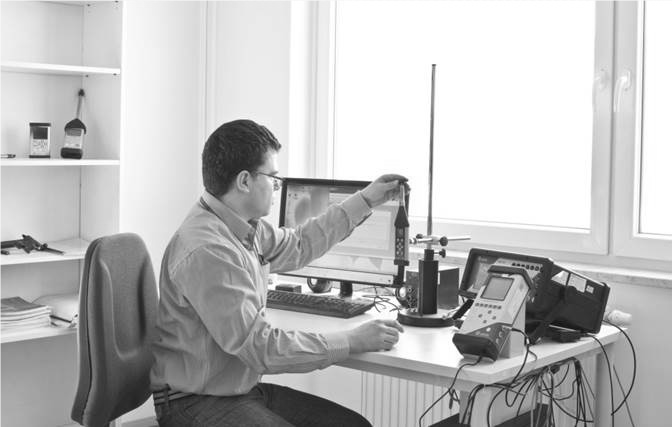
\includegraphics[width=0.8\textwidth]{1_Intro/AP146Laboratory}
    \caption*{\footnotesize Tomado de~\cite{Podgorski2016}}
\end{figure}

Es común encontrar que las organizaciones fabricantes de sonómetros adicionalmente presten servicios de calibración
acreditada (e.g.\ Svantek, Brüel \& Kjær y 01dB), por lo que prácticamente también se pueden denominar OEC\@.
Pero estos OEC en especial, tienen la posibilidad de implementar procedimientos automáticos de calibración sin
limitaciones, puesto que tienen acceso a los comandos de control específicos de sus modelos de sonómetros.
Un ejemplo de eso se encuentra en el artículo de~\cite{Podgorski2016}, en el que se hace una descripción del laboratorio
AP146 en Polonia que pertenece a Svantek y está acreditado por el Centro Polaco de Acreditación (PCA).
En ese artículo se presenta el desarrollo de un \emph{software} de calibración que han validado, desde el que se envían
instrucciones a los instrumentos que generan las señales y a los que las miden, también es posible generar
automáticamente reportes de resultados.
No obstante, sólo es posible usar este \emph{software} con los sonómetros que fabrica la compañía.
Para sonómetros de otras marcas las configuraciones deben hacerse manualmente y por ende el tiempo total de calibración
llega a ser por lo menos el doble.
La figura~\ref{fig:AP146Laboratory} muestra la estación de medición de este laboratorio.

\begin{figure}[!h]
    \caption{Sistema de calibración de sonómetros Type 3630-A desarrollado por Brüel \& Kjær.}
    \label{fig:BK3630A}
    \centering
    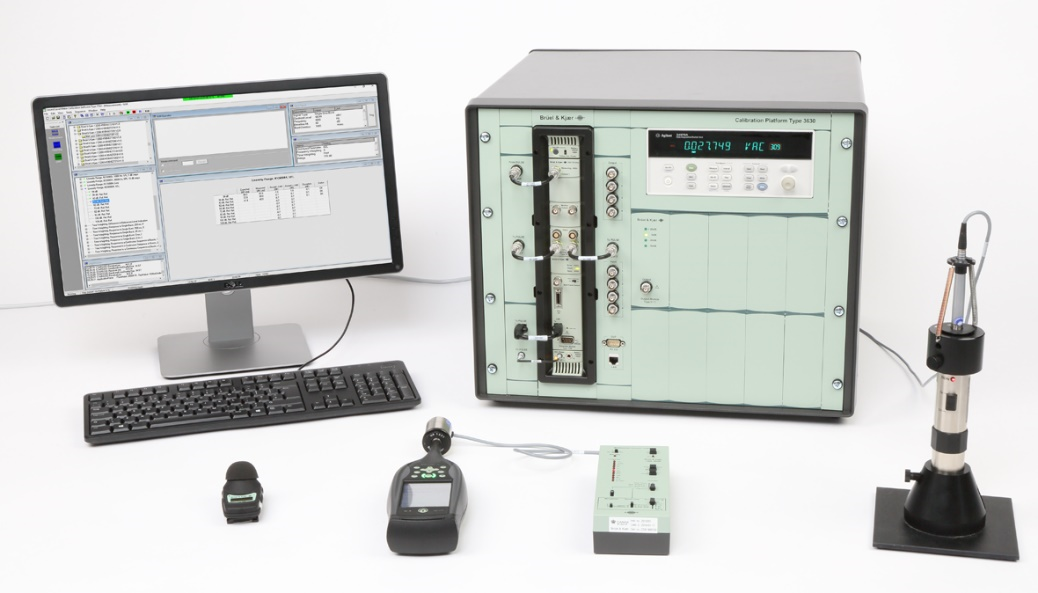
\includegraphics[width=0.8\textwidth]{1_Intro/BK3630A}
    \caption*{\footnotesize Tomado de~\cite{BruelKjaer2000}}
\end{figure}

La figura~\ref{fig:BK3630A} muestra el Type 3630-A, uno de los sistemas de calibración más completo y compacto.
Fue desarrollado por Brüel \& Kjær~\citeyearpar{BruelKjaer2000}, que permite la calibración periódica y la estimación
de incertidumbre de medida para sonómetros Brüel \& Kjær y también de otras marcas.
Además, ofrece la posibilidad de calibrar en modo automático (si el sonómetro dispone de una interfaz serial),
semiautomático (si el sonómetro tiene una salida análoga que corresponda satisfactoriamente con la indicación en
pantalla) y manual (si el sonómetro no cuenta con ninguna salida análoga), con secuencias predefinidas o personalizadas
por el usuario.
Tiene una base de datos de clientes e instrumentos integrada, lo que permite la trazabilidad de los intervalos de
calibración de los patrones de trabajo.
Es capaz de generar certificados de calibración con detallados reportes de resultados.
Permite calibrar dosímetros, calibradores acústicos y filtros.
Sin embargo, por defecto, únicamente tiene disponibles los ensayos de acuerdo con la norma \mbox{IEC 60651} y la
\mbox{IEC 60804}, que quedaron obsoletas rápidamente con el avance tecnológico~\citep{Beyers2014}.
Los ensayos de acuerdo con la \mbox{IEC 61672--3} están disponibles sólo como complementos que el usuario debe comprar.

\subsection{Sistemas de calibración desarrollados por otras organizaciones}
Los anteriores sistemas de calibración desarrollados por los fabricantes más prominentes son sofisticados y costosos,
por lo que los demás OEC, que en su mayoría son organizaciones independientes, deben implementar su propia estación de
trabajo y desarrollar su propio procedimiento de calibración.
El hecho que se desconozca la codificación de control del sonómetro propia de cada fabricante sugiere que lo más seguro
es que este procedimiento sea manual.

Para abordar esta problemática, hay un avance en la automatización del procedimiento de calibración, extendiendo el
alcance a cualquier sonómetro sin importar su modelo o marca, este es el trabajo realizado por~\cite{Zhong2010},
en el que desarrollaron un sistema de calibración implementando reconocimiento de imágenes.
De modo que el resultado es obtenido automáticamente de la indicación en la pantalla del sonómetro, superando así la
limitación más común en los sistemas automáticos de calibración de los fabricantes.
Tal funcionamiento hace de este un sistema mucho más versátil, con el que igualmente se pueden generar de forma
automática los reportes con los resultados de calibración.
Sin embargo, dada su fecha de publicación (2010), está basado en la versión anterior de la
\mbox{IEC 61672--3}~\citeyearpar{IEC_TC29_2013_3}.
Y, por otro lado, utiliza un método de calibración distinto, en el que se requiere una cámara anecóica para calibrar en
campo libre las frecuencias de $\qty{500}{\Hz}$ a $\qty{20}{\kHz}$, un acoplador activo para calibrar en campo de
presión las frecuencias de $\qty{10}{\Hz}$ a $\qty{500}{\Hz}$ y un micrófono patrón de laboratorio para obtener las
respuestas de referencia de los campos, lo que eleva el costo.

La anterior revisión de sistemas de calibración desarrollados por fabricantes y por otros laboratorios indica que hace
falta un sistema de calibración de sonómetros actualizado, versátil, y de bajo costo, pero que no comprometa los
resultados.
Es en esa vía que se planteó este trabajo y se da cumplimiento a los siguientes objetivos.


\section{Objetivos}

\subsection*{General}

Desarrollar un sistema de calibración periódica de sonómetros y calibradores acústicos de conformidad con las normas
\mbox{IEC 61672-3:2013} e {IEC 60942:2017}.
\vfill
\pagebreak

\subsection*{Específicos}

\begin{enumerate}
    \item Formular un modelo en GRAFCET como base para el desarrollo de un sistema de calibración periódica de
    calibradores acústicos.
    \item Implementar las secuencias de comando (a través de bus GPIB) para configurar parámetros de señal y, a su vez,
    recibir resultados de los instrumentos de medición.
    \item Desarrollar un método de reconocimiento de imágenes para detectar los niveles instantáneos ponderados en
    tiempo y en frecuencia desde la pantalla del sonómetro.
    \item Desarrollar un método que permita tener en cuenta la variabilidad de los niveles en pantalla instantáneos
    ponderados en tiempo y en frecuencia del objetivo 3, (mediante mediciones de larga duración), para la estimación
    del mesurando y de la incertidumbre de medición.
\end{enumerate}

\subsection*{Alcance de los objetivos}
El sistema de calibración se implementó para ejecutar las pruebas de calibración de los numerales 9.3 (apoyado en la
IEC 60942), 13, 14 y 16 de la \mbox{IEC 61672--3}.
Los indicadores de interés son los niveles instantáneos con ponderación temporal (\emph{slow} o \emph{fast}) y
ponderación frecuencial ($A$, $C$, o $Z$), i.e. $L_{AF}$,$L_{AS}$,$L_{CF}$,$L_{CS}$,$L_{ZF}$ o $L_{ZS}$, dependiendo
de la prueba y según estén disponibles en el sonómetro sujetos al periodo de actualización de la pantalla del sonómetro.


\section{Estructura del documento}
Antes de introducir el desarrollo técnico de los objetivos, este documento inicia con un capítulo de metodología e
instrumentación en el que se describen el marco normativo y los equipos utilizados en el sistema desarrollado.
Luego, en cumplimiento del tercer objetivo, el capítulo dos explica el diseño e implementación del algoritmo
para el reconocimiento de los caracteres numéricos que representan los niveles de sonido mostrados en la pantalla del
sonómetro.
En el capítulo cuatro se presenta el GRAFCET del objetivo uno y los detalles de implementación del objetivo dos en las
aplicaciones desarrolladas en Python.
En el último capítulo se explican las consideraciones teóricas-experimentales que forman el punto de partida del método
del cuarto objetivo.
Asimismo, se incluye el marco teórico de las cadenas de Markov que son la herramienta esencial del
método y se expone un resultado de ejemplo.
Finalmente, se concluye el documento con una revisión del trabajo realizado y sugerencias para desarrollo futuro.
%  ╔╦╗┌─┐┌┬┐┌─┐┌┬┐┌─┐┬  ┌─┐┌─┐┬┌─┐  ┌─┐  ╦┌┐┌┌─┐┌┬┐┬─┐┬ ┬┌┬┐┌─┐┌┐┌┌┬┐┌─┐┌─┐┬┌─┐┌┐┌
%  ║║║├┤  │ │ │ │││ ││  │ ││ ┬│├─┤  ├┤   ║│││└─┐ │ ├┬┘│ ││││├┤ │││ │ ├─┤│  ││ ││││
%  ╩ ╩└─┘ ┴ └─┘─┴┘└─┘┴─┘└─┘└─┘┴┴ ┴  └─┘  ╩┘└┘└─┘ ┴ ┴└─└─┘┴ ┴└─┘┘└┘ ┴ ┴ ┴└─┘┴└─┘┘└┘

\chapter{Metodología e instrumentación}

En este capítulo se hace una descripción de los instrumentos bajo calibración (calibradores acústicos y sonómetros), seguida de un resumen de los lineamientos de las normas internacionales para las calibraciones periódicas, incluyendo expresiones matemáticas para el cálculo de los voltajes de prueba y otras consideraciones prácticas para los ensayos.
Luego se presentan los patrones y otros instrumentos importantes necesarios para la calibración junto con los esquemas de interconexión.
Finalmente se explican brevemente los comandos para el control remoto de los instrumentos de medición.


\section{Instrumentos bajo calibración}

\subsection{Calibradores acústicos}
De acuerdo con la normativa internacional, un calibrador acústico es un dispositivo diseñado para producir uno o más niveles de presión sonora conocidos (en $\unit{\dB}$ referenciados a $\qty{20}{\micro\Pa}$) a una o más frecuencias especificadas (en $\unit{\Hz}$) cuando se acopla a modelos específicos de micrófono en configuraciones específicas \citepalias{IEC_TC29_2017}.
%
\begin{figure}[!h]
    \caption{Calibrador acústico multifución Brüel \& Kjær 4226.}
    \label{fig:bruel_4226}
    \centering
    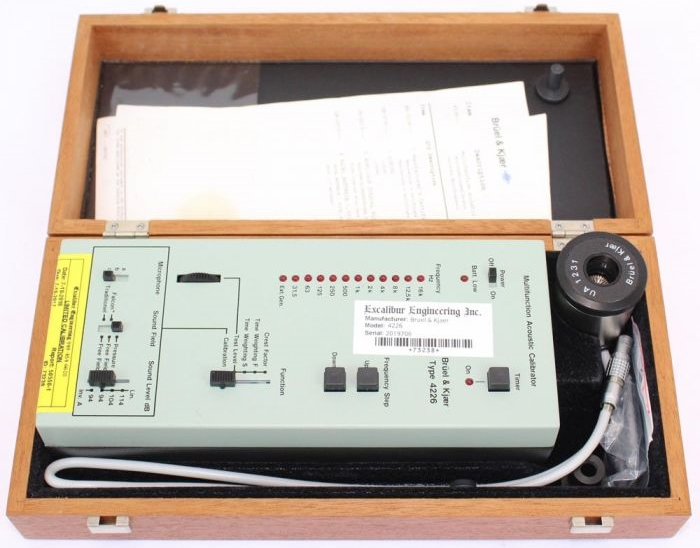
\includegraphics[width=0.35\textwidth]{2_Metodología/Figs/bruel4226}
    \caption*{\footnotesize Imagen tomada de \scriptsize
    \url{https://www.transcat.com/bruel-kjaer-4226-acoustic-calibrator-94-104-and-114db-used}}
\end{figure}

Normalmente, la señal senoidal es generada por algún transductor, como un altavoz o, en el caso de los pistófonos, un pistón mecánico cuyo movimiento genera en la cavidad una velocidad de volumen conocida.
Como ejemplo, en la figura~\ref{fig:bruel_4226} se muestra un calibrador acústico multifunción usado como referencia en muchos laboratorios: el Brüel \& Kjær 4226, que es capaz de generar $\qtylist{94; 104; 114}{\dB}$ en las frecuencias de octava desde $\qty{31.5}{\Hz}$ hasta $\qty{16}{\kHz}$, más la frecuencia de $\qty{12.5}{\Hz}$.

\begin{figure}[!h]
    \caption{Calibrador acústico Brüel \& Kjær 4231 acoplado al micrófono de un sonómetro Brüel \& Kjær 2250.}
    \label{fig:bruel_4231_coupled}
    \centering
    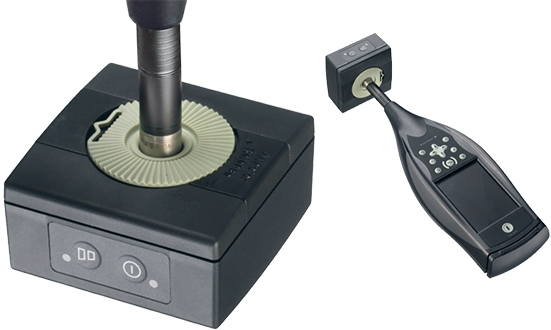
\includegraphics[width=0.45\textwidth]{2_Metodología/Figs/bruel4231coupled}
    \caption*{\footnotesize Imagen tomada de \scriptsize \url{https://www.bksv.com/en/knowledge/blog/sound/getting-started-sound-level-meter}}
\end{figure}
%
Generalmente los calibradores acústicos son empleados para determinar la sensibilidad en campo de presión (típicamente en $\nicefrac{\unit{\mV}}{\unit{\Pa}}$ o en $\unit{\decibel}$ referenciados a $\qty{1}{\V}$) de modelos especificados de micrófonos en configuraciones dadas, pero también es utilizado para verificar o ajustar la sensibilidad de algún dispositivo o sistema de medición acústica.
Un ejemplo de calibrador acoplado para comprobar la indicación de un sonómetro se muestra en la figura~\ref{fig:bruel_4231_coupled}.

La norma \mbox{IEC 60942}~\citeyearpar{IEC_TC29_2017} establece una clasificación de los calibradores según sus especificaciones (límites de aceptación), de la más a la menos restrictiva: Clase LS (\emph{laboratory standard}), clase 1 o clase 2.
La comprobación de que cierto modelo de calibrador cumple con todas las especificaciones normalizadas según su clase la realiza una organización independiente acreditada para hacer pruebas de aprobación de modelo de acuerdo con los lineamientos de la \mbox{IEC 60942} (\mbox{Anexo A},~\citeyear{IEC_TC29_2017}).
Adicionalmente, un usuario de un calibrador acústico debería calibrar periódicamente su instrumento para garantizar la trazabilidad a los estándares nacionales y la confiabilidad de sus resultados.
Esta calibración periódica es llevada a cabo por organismos evaluadores de la conformidad acreditados en \mbox{ISO 17025}~\citeyearpar{ISO_CASCO_2017} para realizar los ensayos periódicos de acuerdo con la \mbox{IEC 60942} (\mbox{Anexo B},~\citeyear{IEC_TC29_2017}).
\vfill

\begin{figure}[!hp]
    \caption{Configuraciones de \emph{hardware} del sonómetro Brüel \& Kjær 2250.}
    \label{fig:bruel_2250_set}
    \centering
    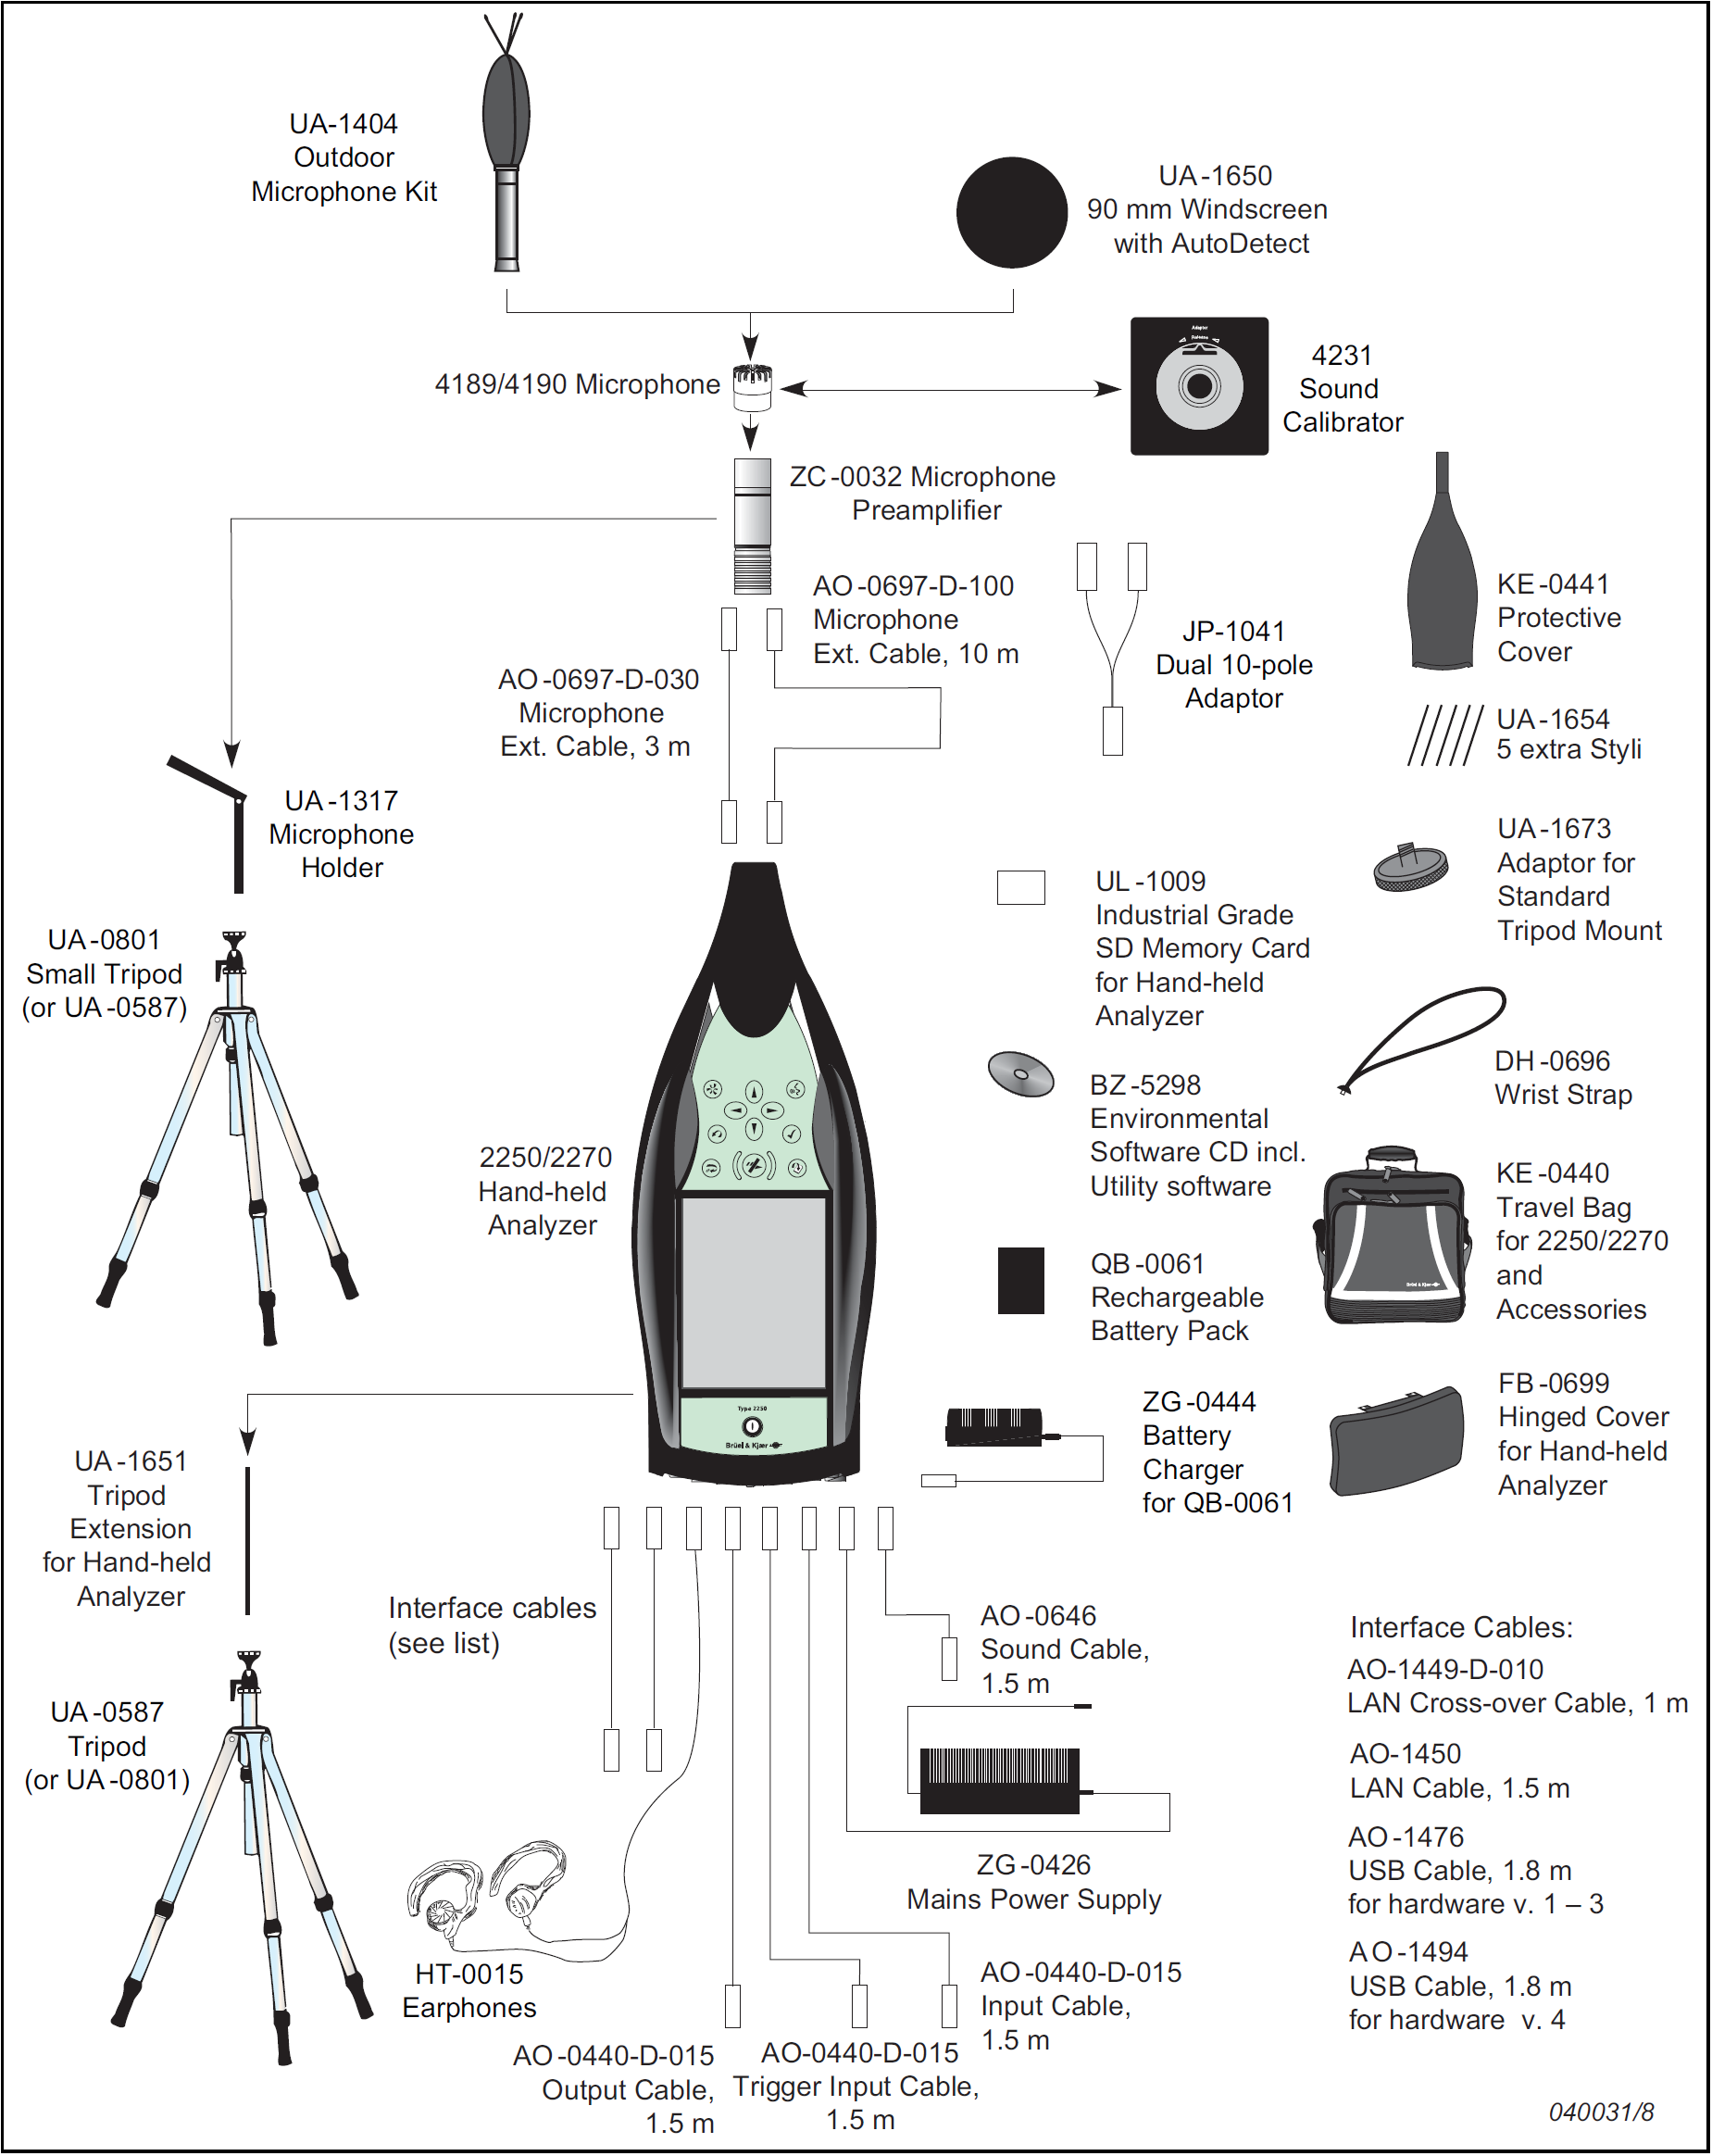
\includegraphics[width=\textwidth]{2_Metodología/Figs/bruel2250set}
    \caption*{\footnotesize Imagen tomada del Manual de Instrucciones \citepalias{Bruel2016}.}
\end{figure}

\subsection{Sonómetros integradores}
Brüel \& Kjær, uno de los fabricantes más prominentes de sonómetros define consistentemente los conceptos básicos sobre dichos instrumentos en uno de sus artículos \citepalias{Bruel2021}.
Básicamente, un sonómetro es un instrumento diseñado para medir niveles de sonido de una forma estandarizada;
su respuesta al sonido se asemeja a la del oído humano y proporciona medidas de niveles de presión sonora objetivas y reproducibles.
Generalmente, los sonómetros son empleados en el monitoreo de ruido proveniente de diversas fuentes sonoras, como plantas industriales, tráfico rodado, aeronáutico o ferroviario, conciertos, etc.
Como se puede ver en la figura~\ref{fig:bruel_2250_set}, un sonómetro típico consta de un micrófono, un preamplificador, una unidad de procesamiento de señal (interna) y una pantalla.
Regularmente el preamplificador hace parte del cuerpo del sonómetro, pero no siempre es el caso;
un sonómetro podría estar provisto de cables de extensión que separen el preamplificador de la unidad de procesamiento.

En cuanto al flujo de señal, el micrófono es un transductor electroacústico que transforma la señal acústica en una señal eléctrica.
La mayoría de los micrófonos empleados en mediciones acústicas son de condensador, y gracias a su construcción es el mejor tipo para garantizar precisión, estabilidad y confiabilidad en los resultados.\ No obstante, la señal eléctrica proporcionada por un micrófono es de baja amplitud (aún con micrófonos de alta gama cuya sensibilidad se encuentra típicamente en el orden de los $50\,\nicefrac{\unit{\mV}}{\unit{\Pa}}$), por lo que se requiere una amplificación para que la unidad de procesamiento manipule la señal en un nivel adecuado, este es el objetivo del preamplificador.
Luego, en la unidad de procesamiento se ejecutan diferentes cálculos a partir de la señal.
Los mínimos requeridos por la norma internacional \mbox{IEC 61672--1}~\citeyearpar{IEC_TC29_2013_1} y utilizados en este proyecto se detallan a continuación.

\begin{figure}[!h]
    \caption{Gráfico de las ponderaciones frecuenciales $A$, $C$ y $Z$.}
    \label{fig:frequency_weightings}
    \centering
    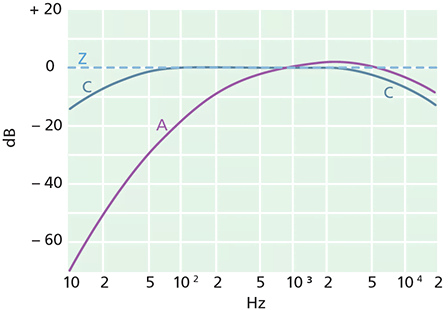
\includegraphics[width=0.54\textwidth]{2_Metodología/Figs/frequency-weighings}
    \caption*{\footnotesize Tomado de \citepalias{Bruel2021}.}
\end{figure}
%
\textbf{Ponderación frecuencial:} Diferencia (como una función especificada de la frecuencia) entre el nivel de la señal ponderada en frecuencia indicado en el dispositivo de presentación de resultados y el nivel correspondiente de una señal de entrada sinusoidal de amplitud constante \citepalias{IEC_TC29_2013_1}.
En la figura~\ref{fig:frequency_weightings} se pueden ver gráficamente las ponderaciones frecuenciales.

Estas ponderaciones frecuenciales estandarizadas $A$, $C$, o $Z$, para las bandas de tercio de octavas están definidas en la \mbox{IEC61672--11} (\mbox{Tabla }~\citeyear{IEC_TC29_2013_1}).
En concreto, cada una de estas ponderaciones modifican la respuesta del sonómetro frente a diferentes frecuencias de sonido.
Por ejemplo, la ponderación $A$ asemeja la respuesta en frecuencia al comportamiento del oído humano en en un rango medio de niveles, tomando como referencia la curva de igual sonoridad de $\qty{40}{\dB}$~\citep{Fletcher1933}, por tal motivo es el más empleado en ruido ambiental y ocupacional.
Pero el oído humano no tiene un comportamiento lineal, y la percepción del sonido varía con el nivel.
La ponderación $C$ está basada en la curva de igual sonoridad de $\qty{100}{\dB}$, por eso esta es empleada en la evaluación de niveles pico de sonidos altos.
Finalmente, la ponderación \emph{zero} $(Z)$ es completamente plana en todo el rango de frecuencias (sin tener en cuenta la respuesta del micrófono).

\textbf{Ponderación temporal:} Es una función exponencial temporal que modifica la respuesta temporal del sonómetro frente a las variaciones en el nivel de presión sonora.
Una comparación entre las respuestas en el tiempo de cada ponderación temporal se muestra en la siguiente figura.
%
\begin{figure}[!h]
    \caption{Gráfico de las respuestas en el tiempo de las ponderaciones temporales \emph{fast}, \emph{slow} e \emph{impulse}.}
    \label{fig:time_weightings}
    \centering
    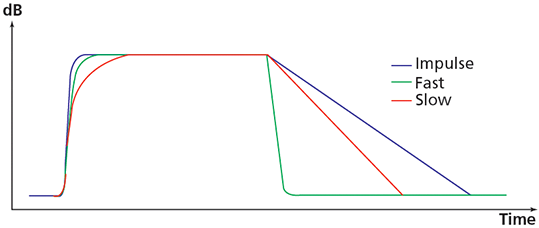
\includegraphics[width=0.55\textwidth]{2_Metodología/Figs/time-weightings}
    \caption*{\footnotesize Tomado de \citepalias{Bruel2021}.}
\end{figure}

Esta función exponencial obedece a una constante de tiempo especificada que depende de la ponderación temporal elegida, bien sea $F$ (\emph{fast}, $\tau_F = \qty{125}{\ms}$), $S$ (\emph{slow}, $\tau_S = \qty{1}{\s}$) o $I$ (\emph{impulse}, $\tau_I = \qty{35}{\ms}$).
Por lo tanto, tal como lo define la norma, para una señal con ponderación $X$, el nivel de sonido con ponderación temporal $Y$ está dado por la siguiente ecuación:
%
\begin{equation}
    \label{eq:time_weighted_level}
    L_{XY}(t) = 10 \log\left(\frac{\frac{1}{\tau_Y}\,
    \int_{-\infty}^t p_X^2\left(\xi\right)\,e^{\nicefrac{-\left(t - \xi\right)}{\tau_Y}}\,\mathrm{d}\xi}
    {p_0^2}\right) \unit{\dB}.
\end{equation}
%
Donde $\tau_Y$ es la constante de tiempo en segundos de la ponderación temporal; $\xi$ es una variable ficticia del tiempo de integración desde un instante de tiempo en el pasado $(-\infty)$ hasta el instante de observación $t$; $p_X\left(\xi\right)$ es la señal de presión acústica instantánea con ponderación frecuencial $X$; y, $p_0$ es el valor de referencia de $\qty{20}{\micro\Pa}$.

Consecuentemente, un nivel de sonido, objeto de evaluación en las pruebas aquí implementadas puede ser $L_{AF}$, $L_{AS}$, $L_{CF}$, $L_{CS}$, $L_{ZF}$ o $L_{ZS}$ para las ponderaciones frecuenciales $A$, $C$, o $Z$ y para las ponderaciones temporales \emph{fast} o \emph{slow}.
El resultado de la medición de nivel de sonido es mostrado directamente en la pantalla del sonómetro o alguna otra herramienta de visualización como una interfaz web.
En algunos sonómetros según su tecnología y disposiciones del fabricante, el resultado de medición es enviado vía serial o en forma de una señal DC o AC de amplitud proporcional al nivel de sonido.

La norma \mbox{IEC 61672--1}~\citeyearpar{IEC_TC29_2013_1} establece una clasificación de los sonómetros según sus especificaciones: clase 1 o clase 2.
La comprobación de que cierto modelo de sonómetro cumple con todas las especificaciones normalizadas, según su clase, la realiza una organización independiente acreditada para hacer pruebas de aprobación de modelo de acuerdo con los lineamientos de la \mbox{IEC61672--22}~\citeyearpar{IEC_TC29_2013_2}.
Pero también un usuario de un sonómetro debería calibrar periódicamente su instrumento para garantizar la trazabilidad a los estándares nacionales y la confiabilidad de sus resultados.
Esta calibración periódica es llevada a cabo por organismos evaluadores de la conformidad acreditados en \mbox{ISO 17025}~\citeyearpar{ISO_CASCO_2017} para realizar los ensayos periódicos de acuerdo con la \mbox{IE61672--3-3}~\citeyearpar{IEC_TC29_2013_3}.

Adicionalmente, la sensibilidad del transductor (micrófono) y la respuesta de los circuitos electrónicos puede variar con el paso del tiempo presentando unas pequeñas derivas o también pueden verse afectadas por las condiciones ambientales como la temperatura y la humedad.
Por esto, es una buena práctica verificar regularmente la sensibilidad del sonómetro (preferiblemente antes y después de cada campaña de medición).
De este modo, el sonómetro será ajustado a un nivel de referencia conocido emitido por un calibrador acústico cuyo nivel tenga trazabilidad metrológica.


\section{Métodos normalizados}

Las especificaciones y metodología de calibración de instrumentación acústica y de vibraciones son normalizadas por el comité técnico 29 de la Comisión Electrotécnica Internacional (IEC) en colaboración con la Organización Internacional de Metrología Legal (OIML).
A continuación, se hará un resumen del proceso de calibración de calibradores acústicos y sonómetros, con especial enfoque en los pasos operativos, más que en las disposiciones preliminares de las normas.

\subsection{Descripción general de la calibración periódica de calibradores acústicos de acuerdo con la \mbox{IEC 60942:2017}}
\label{subsec:acoustic_calibrators_calibration_description}

En la siguiente figura se presenta un diagrama que describe en general el proceso de calibración de calibradores acústicos, el cual es explicado en detalle a continuación.
%
\begin{figure}[h]
    \caption{Diagrama de flujo general de la calibración periódica de calibradores acústicos.}
    \label{fig:acoustic_calibrator_calibration_flowchart}
    \centering
    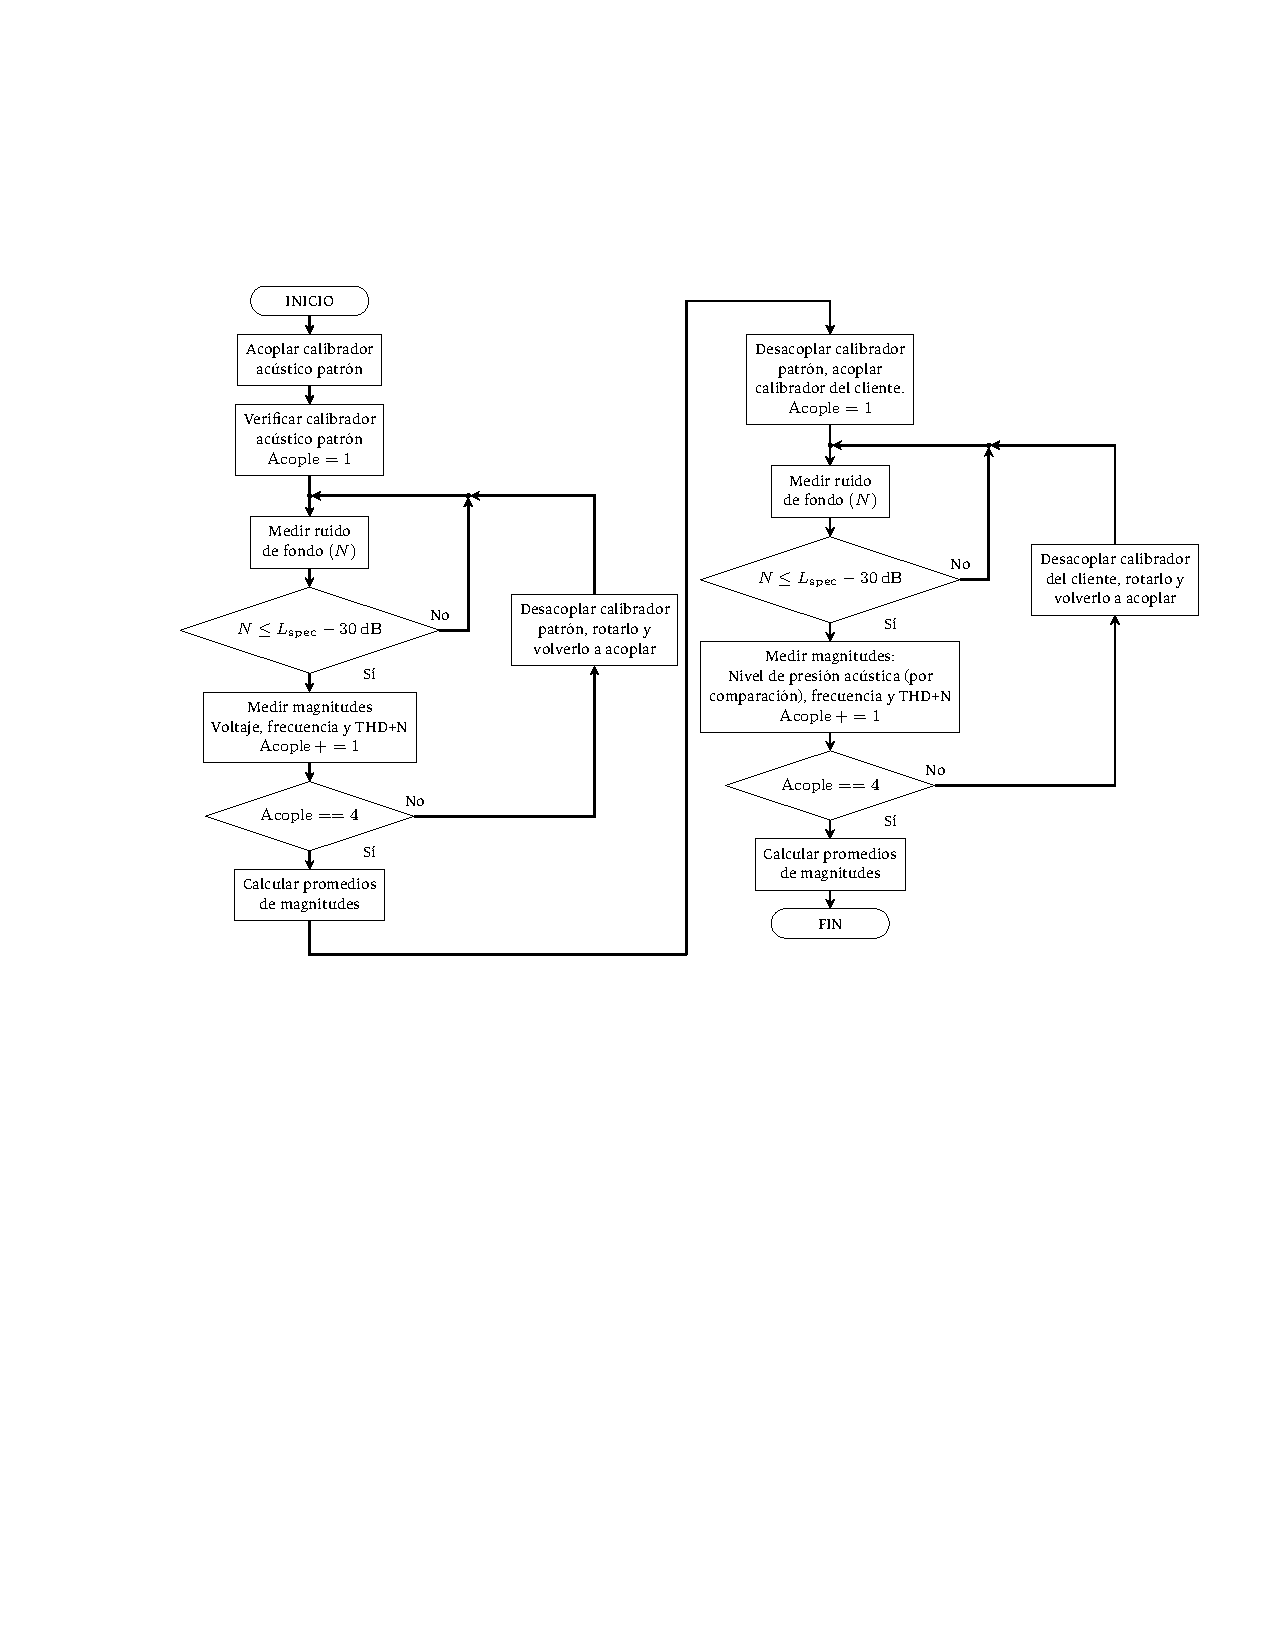
\includegraphics[width=\textwidth]{2_Metodología/IEC60942Flowchart}
    \caption*{\footnotesize Fuente: Elaboración propia.}
\end{figure}

Tal como se describe en la \mbox{IEC 60942} (\mbox{Anexo B},~\citeyear{IEC_TC29_2017}), el calibrador acústico o pistófono con todos sus accesorios necesarios (como adoptadores o barómetro) debe ser entregado junto con el manual de instrucciones, si este es requerido por el laboratorio de calibración.
Luego, se hace una inspección visual del calibrador acústico, verificando que todos los controles están funcionando y que la fuente de alimentación está operando dentro de los límites especificados en el manual de instrucciones.
En seguida, se toman en cuenta o se realizan las siguientes secciones.

\textbf{Orientación para los ensayos}.
Si en el manual de instrucciones se especifica alguna orientación del calibrador acústico, esta debe ser la utilizada en la calibración periódica.

\textbf{Ruido ambiental}.
Para evitar que el ruido ambiental afecte las mediciones, las pruebas sólo se realizan si el nivel de presión sonora con el calibrador acoplado al micrófono (pero con el calibrador apagado) es por lo menos $\qty{30}{\dB}$ por debajo del nivel especificado que se está midiendo.

\textbf{Influencia de las condiciones ambientales}.
Cuando es apropiado, la información suministrada en el manual de instrucciones sobre la influencia de la presión estática debe ser aplicada para corregir el nivel de presión medido a la presión estática de referencia.

\textbf{Nivel de presión sonora}.
Después de acoplar el calibrador acústico al micrófono, se debe dejar el tiempo de estabilización indicado en el manual de instrucciones.
Luego, el nivel de presión sonora generado por el calibrador debe ser medido como un promedio de los valores instantáneos obtenidos durante un periodo (denotado $t_{\mathrm{op}}$) de entre $\qtylist{20;25}{\s}$ de operación.

Para medir el nivel de presión sonora hay propuestos dos métodos en la norma internacional: Usando un micrófono de referencia o usando un calibrador acústico de referencia para comparación.
En este proyecto se utiliza el segundo, en el que el nivel del calibrador bajo prueba es determinado por comparación contra el nivel generado por un calibrador acústico calibrado cuya trazabilidad metrológica esté establecida.
Como la señal a analizar es eléctrica, el nivel de presión se determina como la siguiente diferencia logarítmica:
\begin{equation}
    \label{eq:spl_from_voltage}
    L = L_{\mathrm{ref}} + 20\,\log\left(\frac{\bar{v}}{\bar{v}_{\mathrm{ref}}}\right).
\end{equation}
%
En que $L$ es el nivel de presión sonora del calibrador acústico bajo calibración, $L_{\mathrm{ref}}$ es el nivel de presión certificado del calibrador acústico patrón, y $\bar{v}$ y $\bar{v}_{\mathrm{ref}}$ son el voltaje medio medido con el calibrador del cliente y con el calibrador de referencia durante el tiempo $t_{\mathrm{op}}$ respectivamente.

El nivel de presión sonora debe ser medido al menos tres veces, cada vez acoplando el micrófono y el calibrador acústico antes de la medición y desacoplándolo después.
En cada nuevo acoplamiento se debe rotar el micrófono sobre su eje.
La diferencia absoluta entre el nivel medido medio y el nivel especificado no debe exceder los límites establecidos en la \mbox{IEC 60942} (\mbox{Tabla 2}~\citeyear{IEC_TC29_2017}), según la clase del calibrador y la frecuencia medida.
La medición de nivel de presión sonora debe ser repetida para cada combinación de nivel y frecuencia que indique el manual de instrucciones que cumple con las especificaciones de la norma.

\textbf{Frecuencia}, debe ser medida con el calibrador acoplado al micrófono como un promedio de los valores instantáneos obtenidos durante el tiempo $t_{\mathrm{op}}$, para cada frecuencia disponible en el calibrador, de la cual se indique en el manual que cumple con las especificaciones de la norma.
El valor absoluto de la diferencia porcentual a cada frecuencia medida (ver ecuación~\ref{eq:porcentual_difference}) y la correspondiente frecuencia especificada no debe exceder los límites establecidos en la \mbox{IEC 60942} (\mbox{Tabla 4}~\citeyear{IEC_TC29_2017}), según la clase del calibrador.
%
\begin{equation}
    \label{eq:porcentual_difference}
    \%error = \left|\frac{\bar{f}}{f_{\mathrm{spec}}} - 1\right| \times 100.
\end{equation}
%
En que $\bar{f}$ es la frecuencia media medida durante el tiempo $t_{\mathrm{op}}$ y $f_{\mathrm{spec}}$ es la frecuencia especificada bajo calibración.

\textbf{Distorsión armónica total más ruido (THD+N)}, la distorsión de la señal generada por el calibrador debe medirse con un ancho de banda de $\qty{22.4}{\Hz}$ a $\qty{22.4}{\kHz}$, como un promedio de los valores instantáneos obtenidos durante el tiempo $t_{\mathrm{op}}$, en los niveles máximo y mínimos disponibles a cada frecuencia de los que se indique en el manual que cumple con las especificaciones de la norma.
La THD+N puede ser medida utilizando un filtro de rechazo (medidor de factor de distorsión) o un analizador FFT. La THD+N medida no debe exceder los límites establecidos en la \mbox{IEC 60942} (\mbox{Tabla 7}~\citeyear{IEC_TC29_2017}), según la clase del calibrador.
Es obligatorio que la magnitud medida sea no sólo distorsión armónica total, sino distorsión armónica total \emph{más} ruido, reportada en porcentaje ($\%$).

\subsection{Descripción general de las pruebas periódicas seleccionadas de acuerdo con la \mbox{IEC 61672-3:2013}}
\label{subsec:slm_calibration_description}

\tikzmath{\x1 =1; \x2 = 3/5; \x3 = 3.1/6;}
\definecolor{block_blue}{HTML}{d4e1f5}
\begin{figure}[h]
    \caption{Diagrama de bloques del proceso de medición en la calibración periódica de sonómetros de acuerdo con la \mbox{IEC 61672-3:2013}.}
    \label{fig:slm_calibration_flowchart}
    \centering
    \begin{tikzpicture}[font=\scriptsize, minimum width=1cm, minimum height=1.5cm, align=center]
        \node (process1) at (-10, 0) [draw, process]{Recepción de \\ items de \\ calibración};
        \node (process2) [draw, process, right=\x1cm of process1]{Inspección \\ visual};
        \node (process3) [draw, process, right=\x1cm of process2,
            fill=block_blue]{Verificación \\ del calibrador \\ acústico};
        \node (process4) [draw, process, right=\x1cm of process3, fill=block_blue]{Verificación \\ de fuente de \\ alimentación};
        \node (process5) [draw, process, right=\x1cm of process4]{Ruido \\ intrínseco};
        \node (process6) [draw, process, right=\x1cm of process5]{Indicación a la \\ frecuencia de \\ comprobación de \\ la calibración};
        \node (process7) [draw, process, below=0.3cm of process6]{Una ponderación \\ frecuencial con \\ señales acústicas};
        \node (process8) [draw, process, left=\x2cm of process7, fill=block_blue]{Verificación \\ de fuente de \\ alimentación};
        \node (process9) [draw, process, left=\x2cm of process8, fill=block_blue]{Ponderaciones \\ frecuenciales y \\ temporales a $\qty{1}{\kHz}$};
        \node (process10) [draw, process, left=\x2cm of process9, fill=block_blue]{Ponderación \\ frecuencial con \\ señales eléctricas};
        \node (process11) [draw, process, left=\x2cm of process10, fill=block_blue]{Linealidad en el \\ rango de niveles \\ de referencia};
        \node (process12) [draw, process, below=0.3cm of process1]{Respuesta a \\ trenes de \\ onda};
        \node (process13) [draw, process, below=0.3cm of process12]{Nivel de \\ sonido $C$ \\ de pico};
        \node (process14) [draw, process, right=\x3cm of process13]{Indicación \\ de \\ sobrecarga};
        \node (process15) [draw, process, right=\x3cm of process14]{Estabilidad \\ a niveles \\ elevados};
        \node (process16) [draw, process, right=\x3cm of process15]{Estabilidad a \\ largo plazo};
        \node (process17) [draw, process, right=\x3cm of process16, fill=block_blue]{Verificación \\ de fuente de \\ alimentación};
        \node (process18) [draw, process, right=\x3cm of process17, fill=block_blue]{Estimación de \\ incertidumbre de \\ medición};
        \node (process19) [draw, process, below=0.3cm of process7]{Generación de \\ certificado de \\ calibración};

        \draw [arrow] (process1) -- (process2);
        \draw [arrow] (process2) -- (process3);
        \draw [arrow] (process3) -- (process4);
        \draw [arrow] (process4) -- (process5);
        \draw [arrow] (process5) -- (process6);
        \draw [arrow] (process6.east) -- +(0.3cm, 0cm) |- (process7);
        \draw [arrow] (process7) -- (process8);
        \draw [arrow] (process8) -- (process9);
        \draw [arrow] (process9) -- (process10);
        \draw [arrow] (process10) -- (process11);
        \draw [arrow] (process11) -- (process12);
        \draw [arrow] (process12.west) -- +(-0.3cm, 0cm) |- (process13);
        \draw [arrow] (process13) -- (process14);
        \draw [arrow] (process14) -- (process15);
        \draw [arrow] (process15) -- (process16);
        \draw [arrow] (process16) -- (process17);
        \draw [arrow] (process17) -- (process18);
        \draw [arrow] (process18) -- (process19);
    \end{tikzpicture}
    \caption*{\footnotesize Fuente: Elaboración propia.}
\end{figure}
%
En el diagrama de bloques de la figura~\ref{fig:slm_calibration_flowchart} se presenta de forma general el proceso de calibración periódica de sonómetros.
Los bloques resaltados en azul son los procesos objeto de automatización en este proyecto\footnote{Aún con la automatización de estas actividades, hay tareas que deben realizarse manualmente por el usuario dadas las limitaciones físicas o de la naturaleza misma de los equipos. Por ejemplo, el usuario debe ajustar la orientación del calibrador acústico, encenderlo o apagarlo, configurar en el sonómetro los indicadores en pantalla, etc.}.
A continuación se describen en detalle las etapas en el proceso de calibración.

En principio, de conformidad con la \mbox{IEC 661672--3}~\citeyearpar{IEC_TC29_2013_3}, el sonómetro con todos sus accesorios necesarios (como preamplificador, micrófono, cable de extensión o adaptador de impedancia) debe ser entregado junto con el manual de instrucciones, si este es requerido por el laboratorio de calibración.
Toda la información necesaria para los ensayos periódicos debe estar disponible, como correcciones de campo libre, rangos de medición, niveles de referencia, etc.
Se debe contar con un calibrador acústico conforme con las especificaciones de la \mbox{IEC 60942}~\citeyearpar{IEC_TC29_2017} según su clase, ya sea suministrado por el cliente o por el laboratorio.

Luego, se hace una inspección preliminar del sonómetro y todos sus accesorios, verificando que todos los controles están funcionando, que la pantalla está en buen estado, que no haya acumulación de material extraño en la rejilla o membrana del micrófono y que otros elementos esenciales estén en un funcionamiento adecuado.
Después se verifica que la fuente de alimentación está operando dentro de los límites especificados en el manual de instrucciones.
La fuente de alimentación será verificada nuevamente después de los ensayos con señales acústicas y después de los ensayos con señales eléctricas.
A continuación, se detallan las pruebas que serán efectuadas.
Para todas las pruebas eléctricas se emplea el dispositivo de entrada (acoplador de impedancia) recomendado por el fabricante del sonómetro o uno que tenga una capacitancia similar que emule adecuadamente la carga del micrófono en el preamplificador.

\subsubsection{Indicación a la frecuencia de comprobación de la calibración}
El calibrador acústico entregado por el cliente o proporcionado por el laboratorio se acopla al micrófono del sonómetro, y, si es necesario, se ajusta el sonómetro para indicar el nivel de presión acústica requerido en las condiciones ambientales en las que se realizan los ensayos.
Las indicaciones antes y después del ajuste deben registrarse.
Se debe tomar en cuenta el efecto de la presión estática sobre el calibrador acústico empleado.
Este calibrador ya debió haber sido verificado previamente, según el procedimiento descrito en la sección~\ref{subsec:acoustic_calibrators_calibration_description}.

Después de haber ajustado el sonómetro en respuesta al nivel generado por el calibrador, un paso necesario (antes de continuar con las otras pruebas) es determinar el voltaje que produce una indicación del nivel de referencia.
La siguiente ecuación es empleada para determinar ese voltaje:
%
\begin{equation}
    \label{eq:reference_voltage}
    v_{\mathrm{ref}} = 10\,\hat{\mkern6mu}\left(\frac{L_{v,l}+\nicefrac{\left(L_{v,u} - L_{v,l}\right)}{2}}{20}\right).
\end{equation}
%
Donde $v_{\mathrm{ref}}$ es el voltaje medio en una escala logarítmica que produce una indicación del nivel de referencia, $L_{v,l}$ es el nivel de voltaje inferior del intervalo que produce una indicación del nivel de referencia, y $L_{v,u}$ el nivel de voltaje superior.
Los niveles de voltaje son referenciados a $\qty{1}{\V}$.
En concreto, este voltaje de referencia es el voltaje en la mitad (en una escala logarítmica) de un intervalo de voltajes que producen todos una misma indicación del nivel de referencia.
Con el voltaje de referencia se calculan los voltajes correspondientes a los niveles de señal en las demás pruebas.

\subsubsection{Ponderaciones frecuenciales y temporales a 1 kHz}
Se utiliza una señal eléctrica continua de $\qty{1}{\kHz}$ con una amplitud tal que produzca una indicación del nivel de referencia en el sonómetro $\left(\text{i.e. } v_{\mathrm{ref}}\right)$  y se siguen los pasos a continuación:
%
\begin{description}
    \item[PFT-1] Registrar el nivel indicado en las ponderaciones frecuenciales $A$, $C$ y $Z$ (según estén disponibles) con el sonómetro ajustado en ponderación temporal $F$ o nivel promediado en el tiempo\footnote{Como en este trabajo se busca reconocer el resultado instantáneo mostrado en pantalla, el nivel elegido preferiblemente es el que tiene ponderación temporal $F$.}; i.e. $L_{AF}, L_{CF}, L_{ZF}, L_{Aeq}, L_{Ceq}$ o $L_{Zeq}$.

    \item[PFT-2\label{itm:time_frequency_weight_registration}] Registrar el nivel indicado en las ponderaciones temporales $F$ y $S$, y el nivel promediado en el tiempo\footnote{El nivel promediado en el tiempo sólo sería posible registrarlo automáticamente si este es mostrado en pantalla.} (según estén disponibles) con el sonómetro ajustado en ponderación frecuencial $A$; i.e. $L_{AF}, L_{AS}$ o $L_{Aeq}$.

    \item[PFT-3] Calcular las desviaciones de los niveles ponderados en frecuencia $C$ y $Z$ respecto al ponderado en frecuencia $A$ del paso 1.
    Estas desviaciones no deben superar los límites de aceptación de $\pm\qty{0.2}{\dB}$.

    \item[PFT-4] Calcular las desviaciones del nivel promediado en el tiempo y del nivel con ponderación temporal $S$, respecto al nivel con ponderación temporal $F$ del paso~\ref{itm:time_frequency_weight_registration}.
    Estas desviaciones no deben superar los límites de aceptación de $\pm\qty{0.1}{\dB}$.
\end{description}

\subsubsection{Ponderaciones frecuenciales con señales eléctricas}

Se utilizan señales eléctricas sinusoidales continuas para todas las ponderaciones frecuenciales reguladas en la \mbox{IEC 61672--1}~\citeyearpar{IEC_TC29_2013_1} (que estén disponibles en el sonómetro).
Y se siguen los pasos a continuación:
%
\begin{description}
    \item[PFSE-1] Se ajusta el sonómetro para mostrar niveles de sonido con ponderación temporal $F$, niveles promediados en el tiempo o niveles de exposición sonora \footnote{Como en este trabajo se busca reconocer el resultado instantáneo mostrado en pantalla, el nivel elegido es preferiblemente el que tiene ponderación temporal $F$.}.

    \item[PFSE-2] Se ajusta el sonómetro en el rango de niveles de referencia y se envía una señal de $\qty{1}{\kHz}$ cuya amplitud produzca una indicación en el sonómetro que sea $\qty{45}{\dB}$ menos que el límite superior indicado en el manual de instrucciones para el rango de funcionamiento lineal a $\qty{1}{\kHz}$.

    Para automatizar este paso, se usa la siguiente ecuación:
%
    \begin{equation}
        \label{eq:voltage_1khz}
        v_{\qty{1}{\kHz}} = 10\,\hat{\mkern6mu}
        \left(\frac{20\,\log\left(v_{\mathrm{ref}}\right) + L_{\mathrm{ref}} - \left(L_{u@\qty{1}{\kHz}} - 45\right)}{20}\right).
    \end{equation}
%
    En que $v_{\qty{1}{\kHz}}$ es el voltaje que produce una indicación de $\qty{45}{\dB}$ menos que el límite superior del rango lineal a $\qty{1}{\kHz}$; $v_{\mathrm{ref}}$ es el voltaje que produce una indicación del nivel de referencia $L_{\mathrm{ref}}$; y, $L_{u@\qty{1}{\kHz}}$ es el límite superior del rango lineal a $\qty{1}{\kHz}$ especificado en el manual de instrucciones.

    \item[PFSE-3] Se registran los niveles de las señales de entrada y las correspondientes indicaciones.
    Para sonómetros clase 1 en las nueve frecuencias nominales en intervalos de octava de $\qty{63}{\Hz}$ a $\qty{16}{\kHz}$.
    Para sonómetros clase 2 en las ocho frecuencias nominales en intervalos de octava de $\qty{63}{\Hz}$ a $\qty{8}{\kHz}$.

    En frecuencias diferentes a $\qty{1}{\kHz}$ el voltaje de la señal de entrada se determina mediante
%
    \begin{equation}
        \label{eq:voltage_by_frequency}
        v_f = 10\,\hat{\mkern6mu}\left(\frac{20\,\log\left(v_{\qty{1}{\kHz}}\right) - W_{X,f}}{20}\right).
    \end{equation}
%
    En que $v_f$ es el voltaje de la señal a la frecuencia $f$, $v_{\qty{1}{\kHz}}$ es el voltaje del paso anterior y $W_{X,f}$ es el factor de la ponderación frecuencial elegida $X$ para la frecuencia $f$.

    \item[PFSE-4] Se calculan las ponderaciones frecuenciales relativas como $L_{f} - L_{\qty{1}{\kHz}}$, i.e.\ el nivel indicado a una frecuencia de ensayo menos el nivel indicado a $\qty{1}{\kHz}$.

    \item[PFSE-5] Aplicar factores de corrección a las ponderaciones frecuenciales relativas del paso anterior que den cuenta de:
%
    \begin{description}
        \item[PFSE-5.1] La desviación de la respuesta en frecuencia en campo libre o para incidencia aleatorio de un micrófono en la dirección de referencia respecto a una respuesta en frecuencia uniforme.
        \item[PFSE-5.2] Los efectos de las reflexiones en la carcasa del sonómetro y de la difracción del sonido alrededor del micrófono y del amplificador.
        \item[PFSE-5.3] Si aplica, la influencia de la pantalla antiviento y de cualquier accesorio que sea parte de la configuración normal del sonómetro.
    \end{description}

    \item[PFSE-6] Las ponderaciones frecuenciales relativas corregidas son las desviaciones respecto a los objetivos de diseño según la ponderación frecuencial bajo calibración y no deben exceder los límites de aceptación dados en la \mbox{IEC 61672--1} (\mbox{Tabla 3}~\citeyear{IEC_TC29_2013_1}).
\end{description}

\subsubsection{Linealidad de nivel en el rango de niveles de referencia}
Se utilizan señales eléctricas sinusoidales continuas a una frecuencia de $\qty{8}{\kHz}$ con el sonómetro ajustado en el rango de niveles de referencia, en ponderación frecuencial $A$, y con ponderación temporal $F$ o un nivel promediado en el tiempo, i.e. $L_{AF}$ o $L_{Aeq}$, y se siguen los pasos a continuación:
%
\begin{description}
    \item[LNRR-1] Comenzar con una señal de entrada cuya amplitud produce el punto de partida para los ensayos de linealidad a $\qty{8}{\kHz}$ especificado en el manual de instrucciones.
    Y registrar el nivel indicado.

    \item[LNRR-2] Aumentar el nivel de la señal de entrada en saltos de $\qty{5}{\dB}$ desde el punto de partida hasta un nivel que se encuentre dentro de $\qty{5}{\dB}$ por debajo del límite superior del rango de funcionamiento lineal a $\qty{8}{\kHz}$ especificado en el manual.
    Luego, aumentar en saltos de $\qty{1}{\dB}$ hasta, pero sin incluir, la primera indicación de sobrecarga.
    Se deben registrar las indicaciones del sonómetro en cada punto.

    \item[LNRR-3] Disminuir el nivel de la señal de entrada en saltos de $\qty{5}{\dB}$ desde el punto de partida hasta un nivel que se encuentre dentro de $\qty{5}{\dB}$ por encima del límite inferior del rango de funcionamiento lineal a $\qty{8}{\kHz}$ especificado en el manual.
    Luego, disminuir en saltos de $\qty{1}{\dB}$ hasta, pero sin incluir, la primera indicación de ``por debajo del rango".
    Se deben registrar las indicaciones del sonómetro en cada punto.

    \item[LNRR-4] Calcular las desviaciones de nivel como la diferencia entre el nivel indicado y el nivel previsto.
    Estas desviaciones no deben superar los límites de $\pm\qty{0.8}{\dB}$ para la clase 1 o de $\pm\qty{1.1}{\dB}$ para la clase 2.
\end{description}

Para automatizar esta prueba, el voltaje en el punto de partida se determina como
%
\begin{equation}
    \label{eq:voltaje_start_point}
    v_{L_{\mathrm{start}}} = 10\,\hat{\mkern6mu}
    \left(\frac{20\,\log\left(v_{\mathrm{ref}}\right) +
    L_{\mathrm{start}} - L_{\mathrm{ref}} -
    W_{A,\qty{8}{\kHz}} - E_{A,\qty{8}{\kHz}}}{20}\right).
\end{equation}
%
En que $v_{L_{\mathrm{start}}}$ es el voltaje que causa una indicación del nivel en el punto de partida $L_{\mathrm{start}}$; $v_{\mathrm{ref}}$ es el voltaje que produce una indicación del nivel de referencia, $W_{A,\qty{8}{\kHz}}$ es el factor estandarizado de la ponderación $A$ en la frecuencia de $\qty{8}{\kHz}$ que tiene el valor de $\qty{-1.1}{\dB}$ y $E_{A,\qty{8}{\kHz}}$ es la ponderación relativa a $\qty{1}{\kHz}$ (sin corregir), obtenida en la prueba de ponderaciones frecuenciales en la frecuencia de $\qty{8}{\kHz}$ en la ponderación frecuencial $A$.%, y $R_{\mathrm{FF},\qty{8}{\kHz}}$ es la corrección de campo libre para la frecuencia de $\qty{8}{\kHz}$.

Luego, a partir de ese voltaje en el punto de partida, el voltaje $v_{L_{\mathrm{prev}}}$ para cada punto de calibración o nivel previsto $L_{\mathrm{prev}}$ a lo largo del rango de niveles, se calcula como:
%
\begin{equation}
    \label{eq:voltage_linearity}
    v_{L_{\mathrm{prev}}} = 10\,\hat{\mkern6mu}
    \left(\frac{20\,\log\left(v_{L_{\mathrm{start}}}\right) + L_{\mathrm{prev}} - L_{\mathrm{start}}}{20}\right).
\end{equation}


\section{Instrumentación}\label{sec:instrumentacion}

Los instrumentos presentados a continuación fueron elegidos teniendo en cuenta los requisitos metrológicos para obtener resultados confiables y trazables, como también asegurando que tengan las prestaciones mínimas para implementar el control remoto desde un ordenador.

\begin{figure}[!h]
    \caption{Esquema de conexiones de los instrumentos para la calibración periódica de calibradores acústicos.}
    \label{fig:IEC60942_connections}
    \begin{subfigure}[t]{0.59\textwidth}
        \centering
        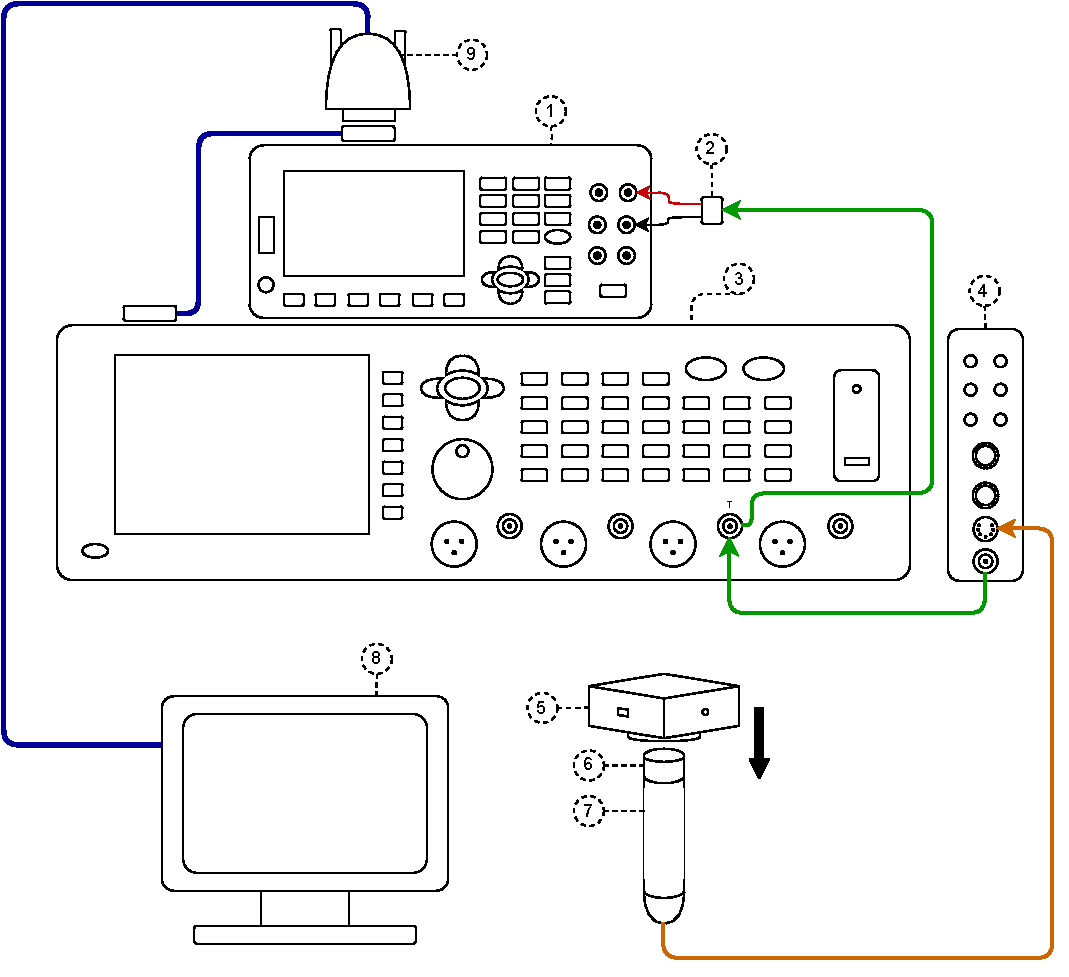
\includegraphics[width=0.95\textwidth]{2_Metodología/Figs/IEC60942connections}
    \end{subfigure}
    \hfill
    \begin{subfigure}[t]{0.4\textwidth}
        \centering
        \begin{tikzpicture}
            \node [draw]{\vbox{\scriptsize{
                \begin{enumerate}
                    \item Multímetro digital Keysight 34461A
                    \item Convertidor BNC-Banana
                    \item Analizador de audio Keysight U8903B
                    \item Módulo de poder GRAS 12AK
                    \item Calibrador acústico Brüel \& Kjær 4231
                    \item Micrófono patrón de trabajo GRAS 40CE
                    \item Preamplificador 01dB PRE22
                    \item Computador
                    \item Interfaz GPIB Keysight 82357B
                \end{enumerate}}
            \raggedright\qquad\textbf{\color{blue} —} Conexión GPIB \\
            \raggedright\qquad\textbf{\color{orange} —} Conexión Lemo 7 \\
            \raggedright\qquad\textbf{\color{oliva_green} —} Conexión BNC}};
        \end{tikzpicture}
    \end{subfigure}
    \caption*{\footnotesize Fuente: Elaboración propia.}
\end{figure}

\subsection{Patrones e instrumentos para la calibración periódica de calibradores acústicos}

La interconexión propuesta de los instrumentos empleados en la calibración de calibradores acústicos se presenta en la figura~\ref{fig:IEC60942_connections}.
A continuación se describen las características de cada instrumento.

\begin{figure}[!h]
    \caption{Patrones acústicos para la calibración de calibradores acústicos.}
    \centering
    \begin{subfigure}[t]{0.49\textwidth}
        \centering
        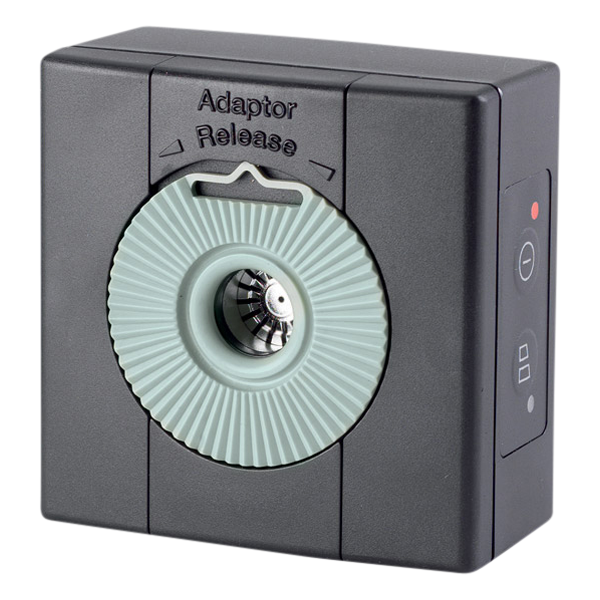
\includegraphics[height=4cm]{2_Metodología/Figs/bruel4231}
        \caption{Calibrador acústico Brüel \& Kjær 4231 usado como patrón de laboratorio.}
        \label{fig:bruel_4231}
    \end{subfigure}
    \hfill
    \begin{subfigure}[t]{0.49\textwidth}
        \centering
        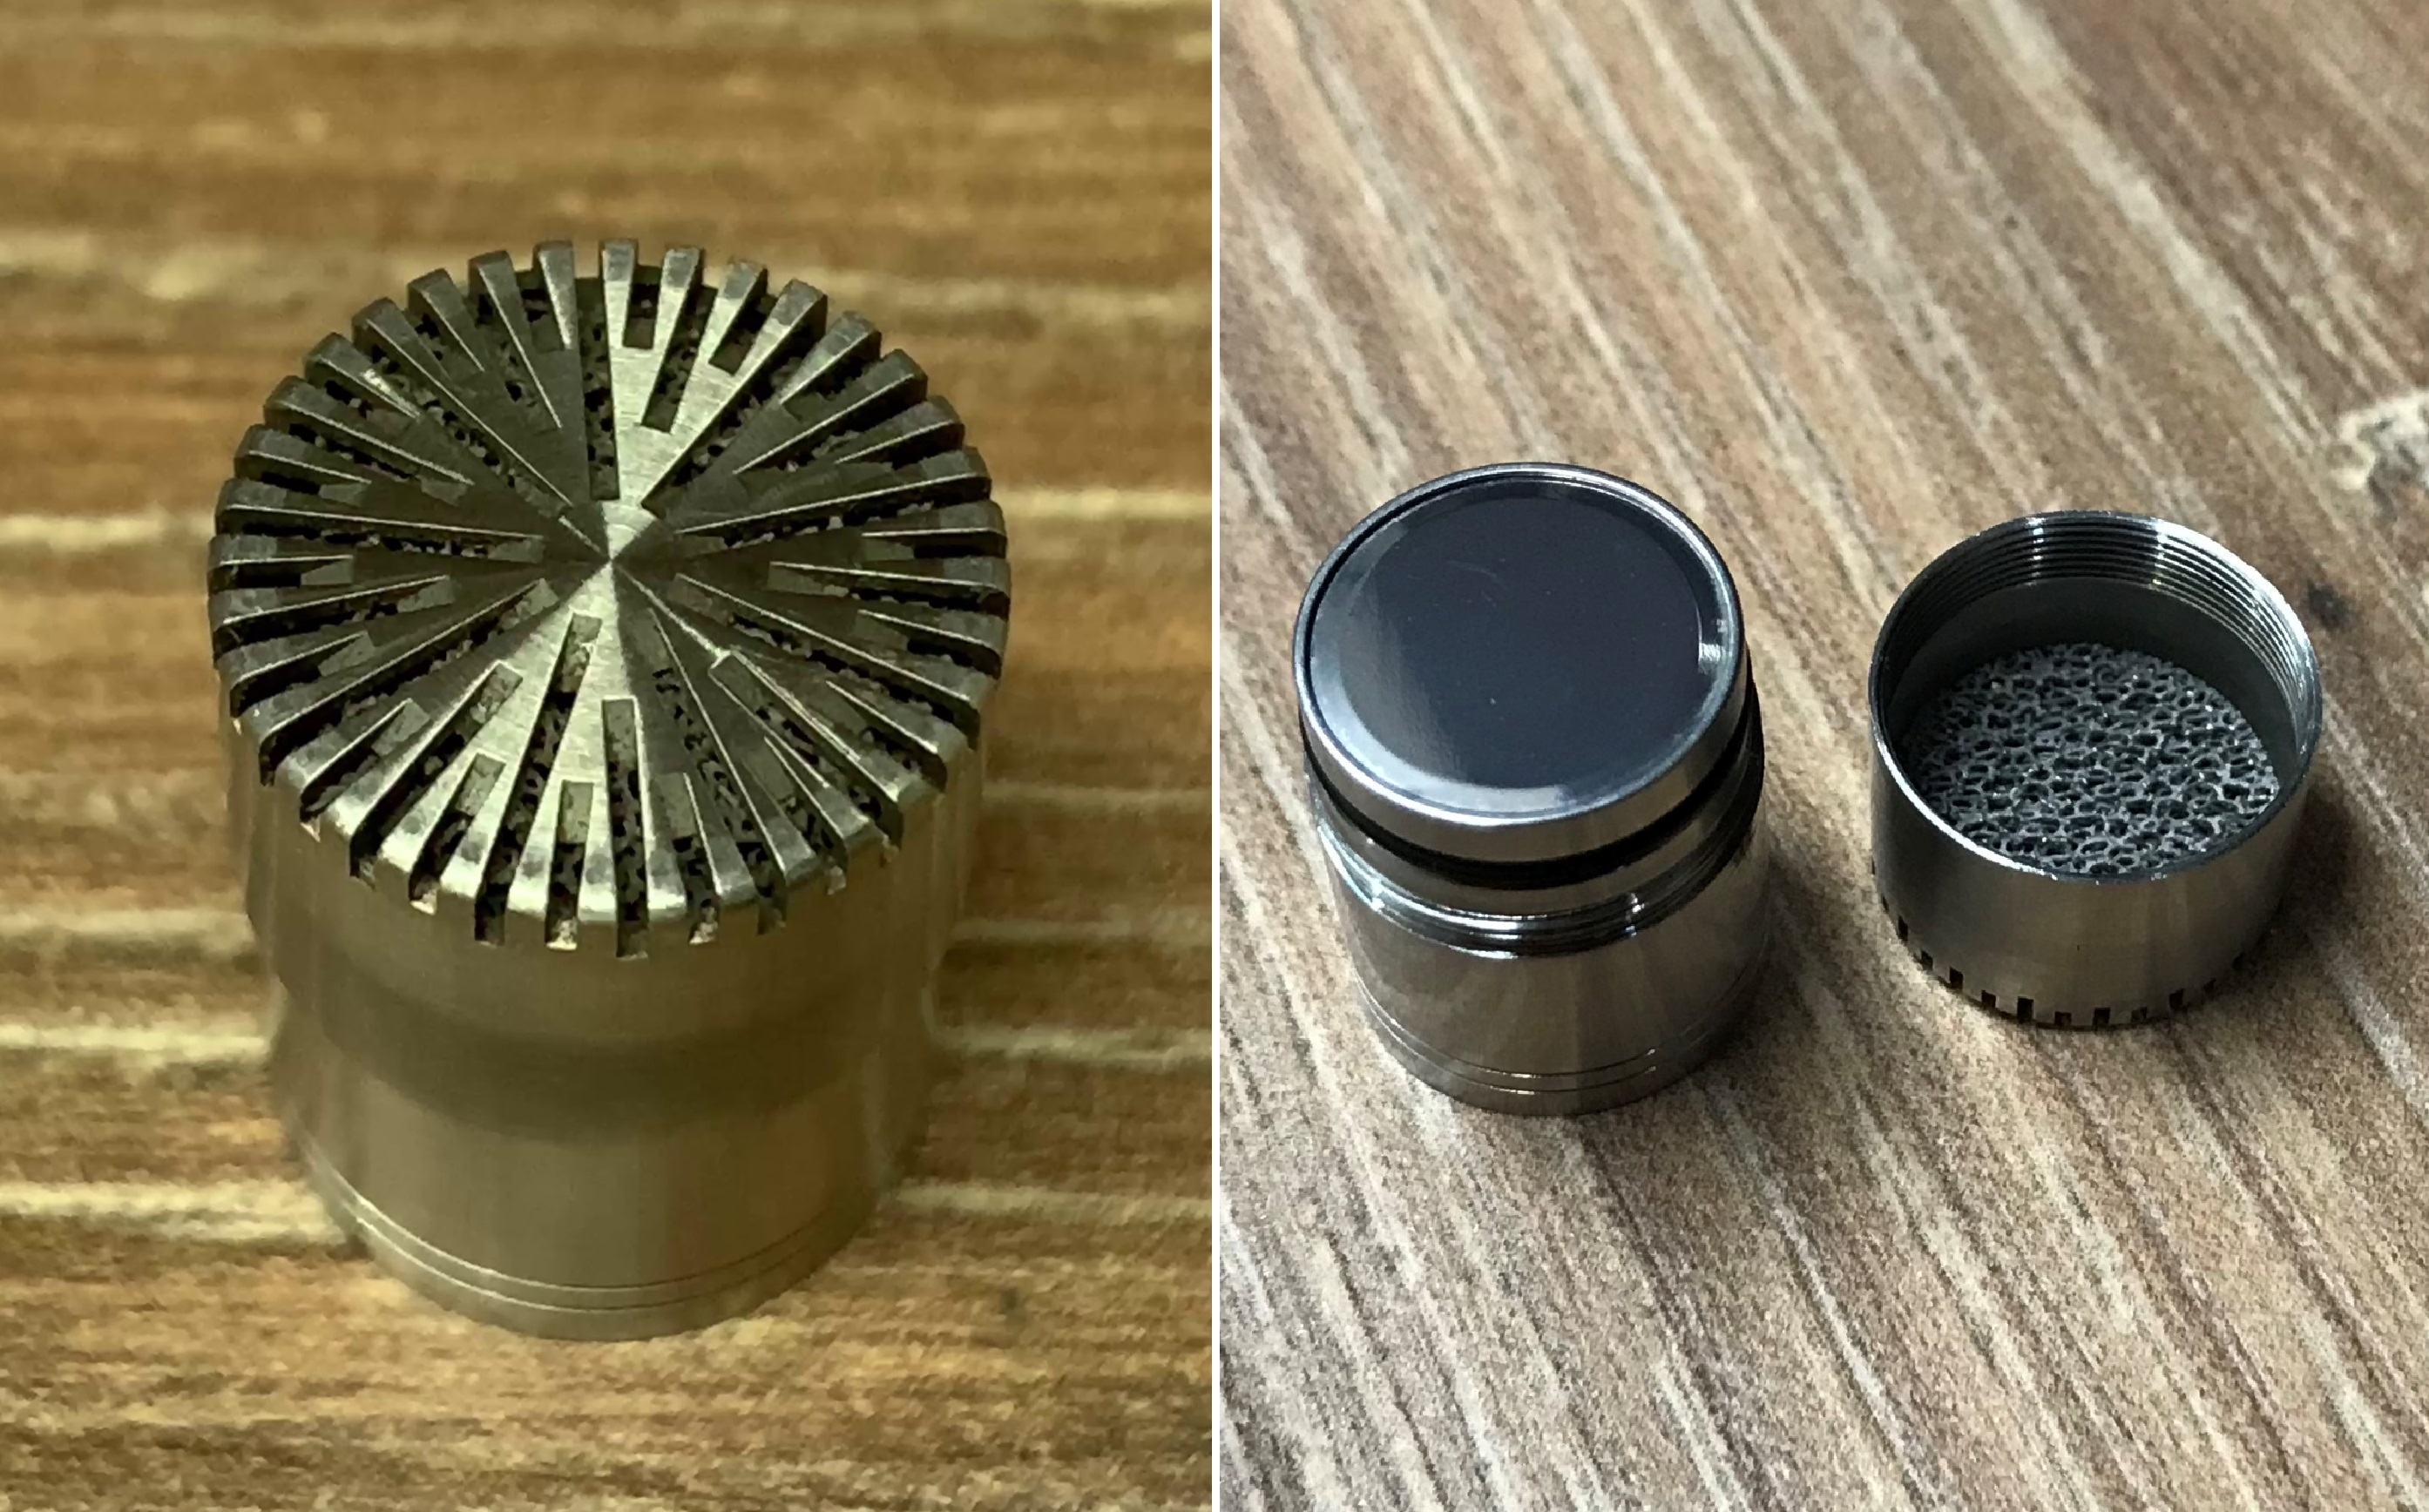
\includegraphics[height=4cm]{2_Metodología/Figs/gras40CE}
        \caption{Micrófono patrón de trabajo GRAS 40CE.}
        \label{fig:gras_40CE}
    \end{subfigure}
\end{figure}
%
\begin{figure}[!h]
    \caption{Instrumentos para adecuación de la señal eléctrica.}
    \centering
    \begin{subfigure}[t]{0.6\textwidth}
        \centering
        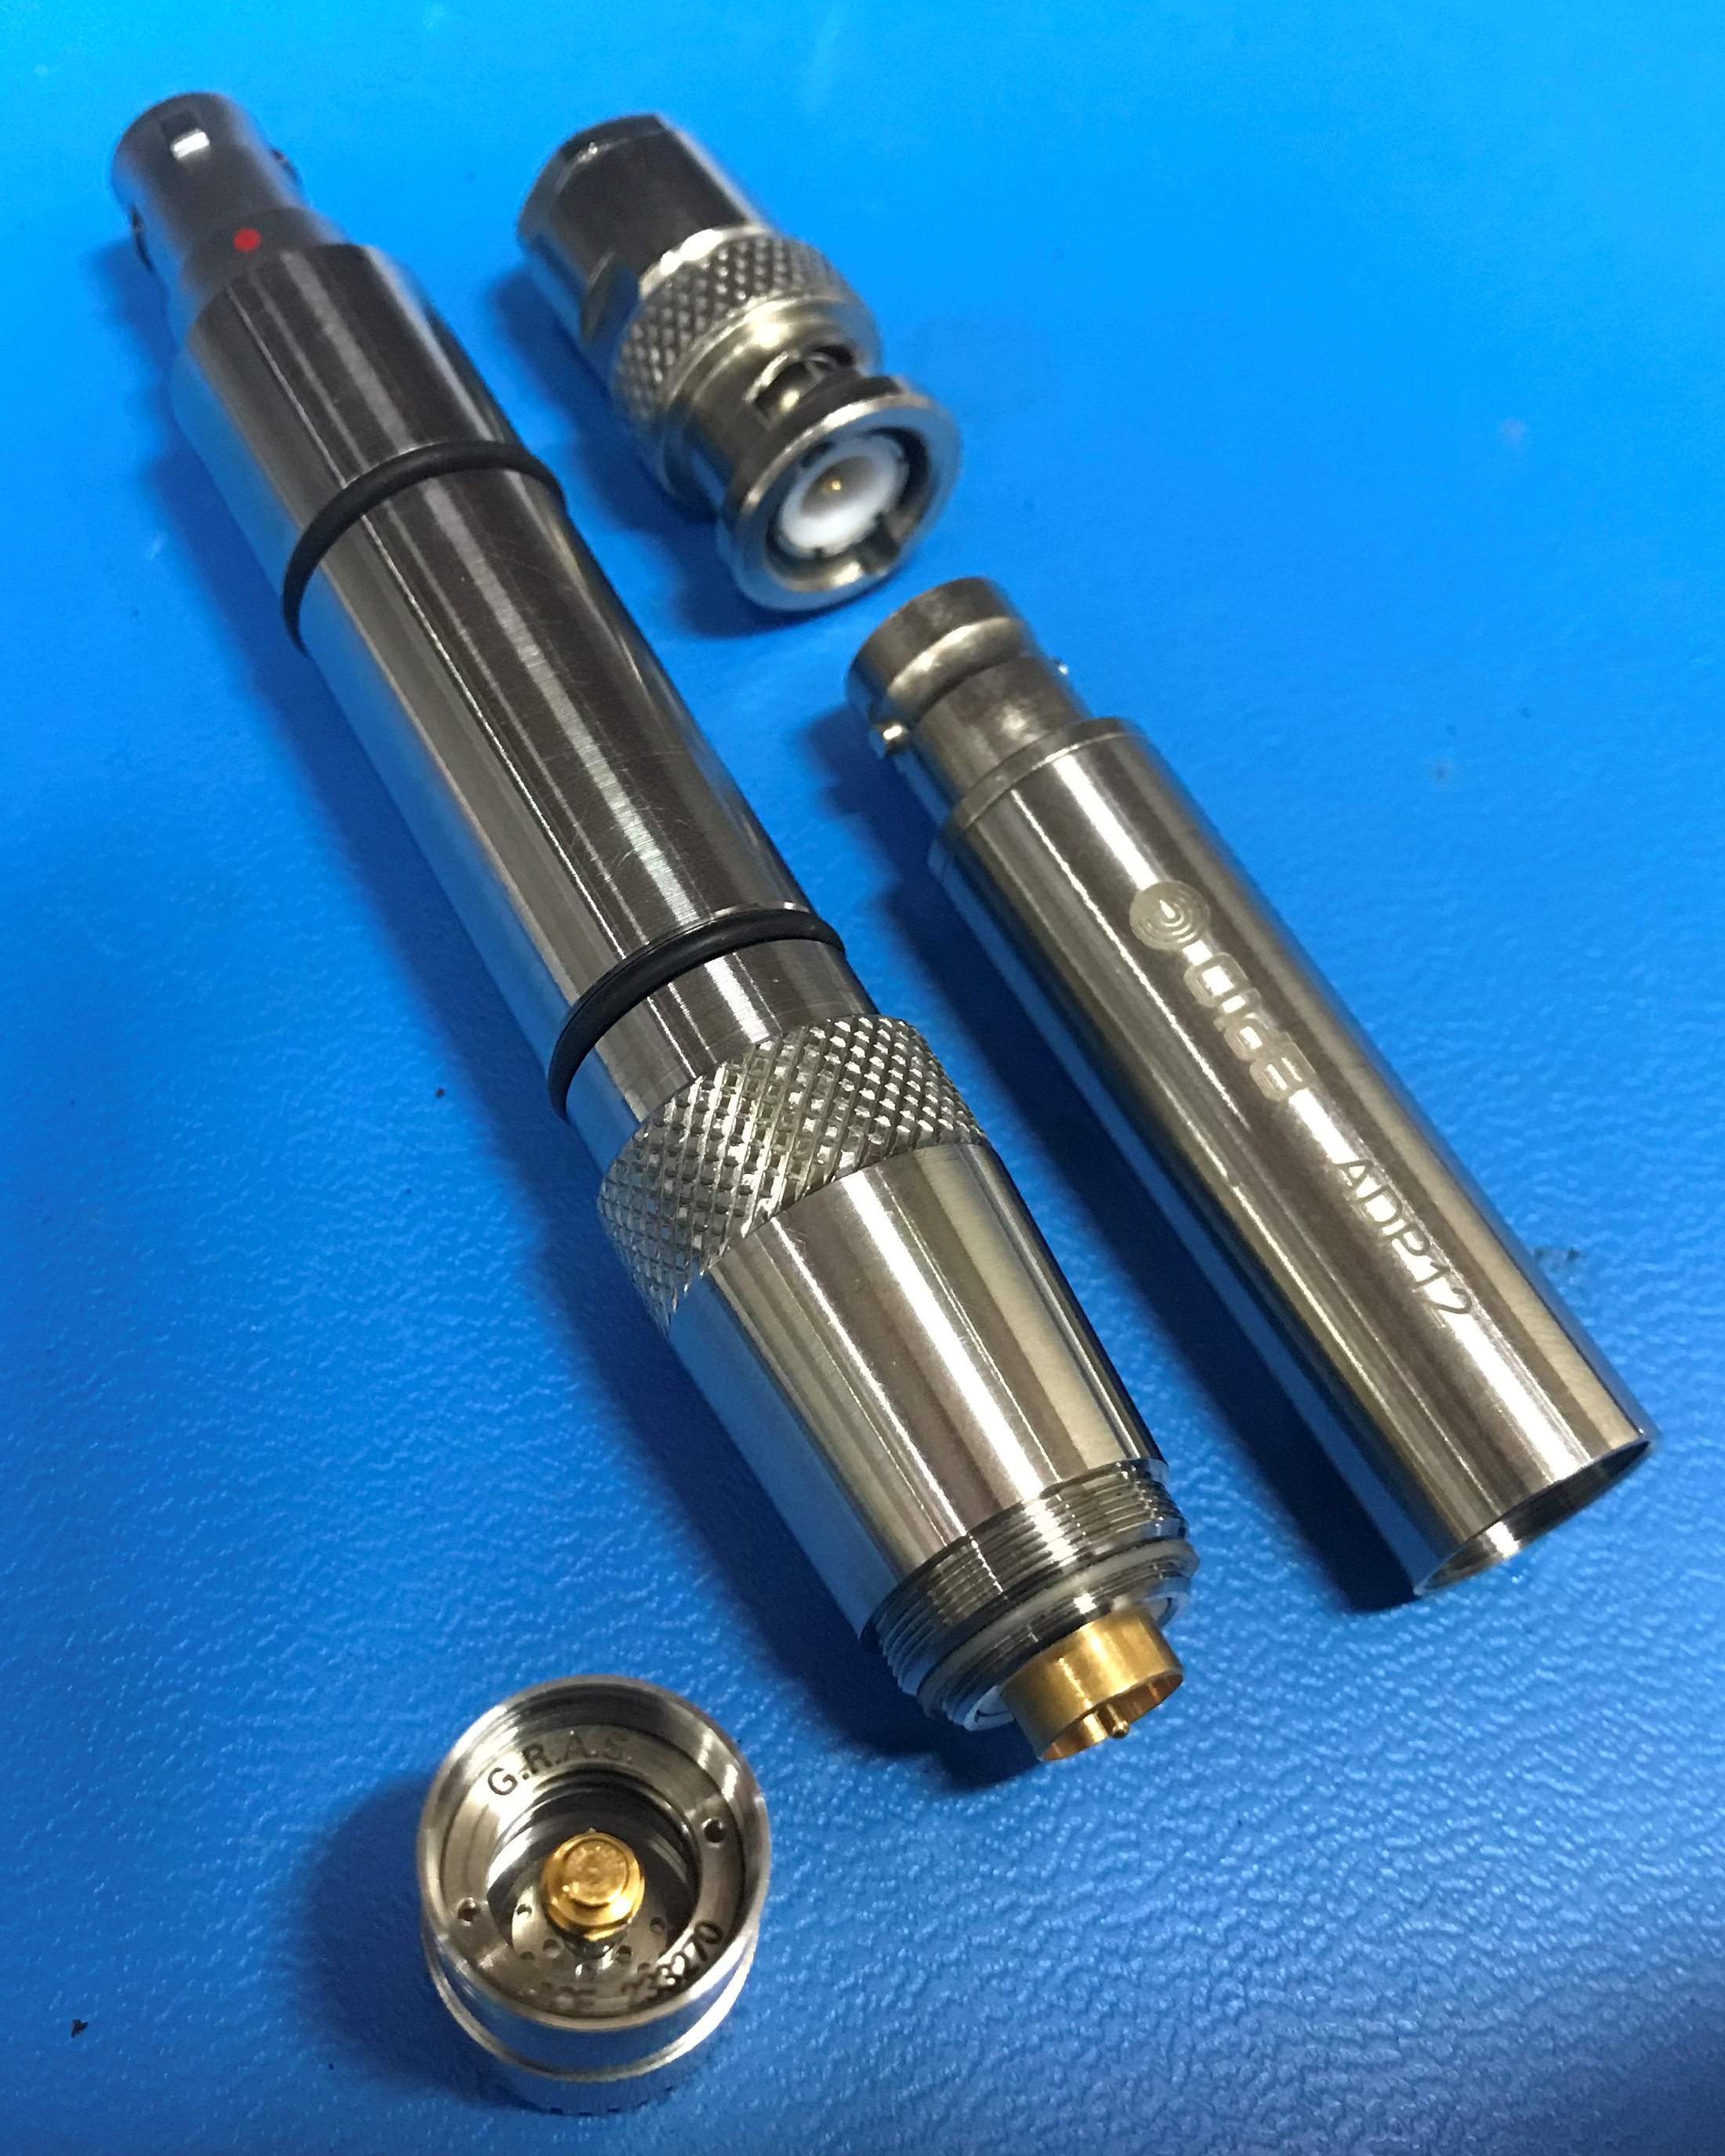
\includegraphics[height=7cm]{2_Metodología/Figs/PRE2201dB}
        \caption{Vista inferior del micrófono GRAS 40CE (izquierda abajo),
            preamplificador para micrófonos de $\nicefrac{1}{2}''$ 01dB PRE22 (medio)
            y adaptador de impedancia 01dB ADP12 con su terminal de aterrizaje (derecha).}
        \label{fig:PRE22_01dB}
    \end{subfigure}
    \hfill
    \begin{subfigure}[t]{0.38\textwidth}
        \centering
        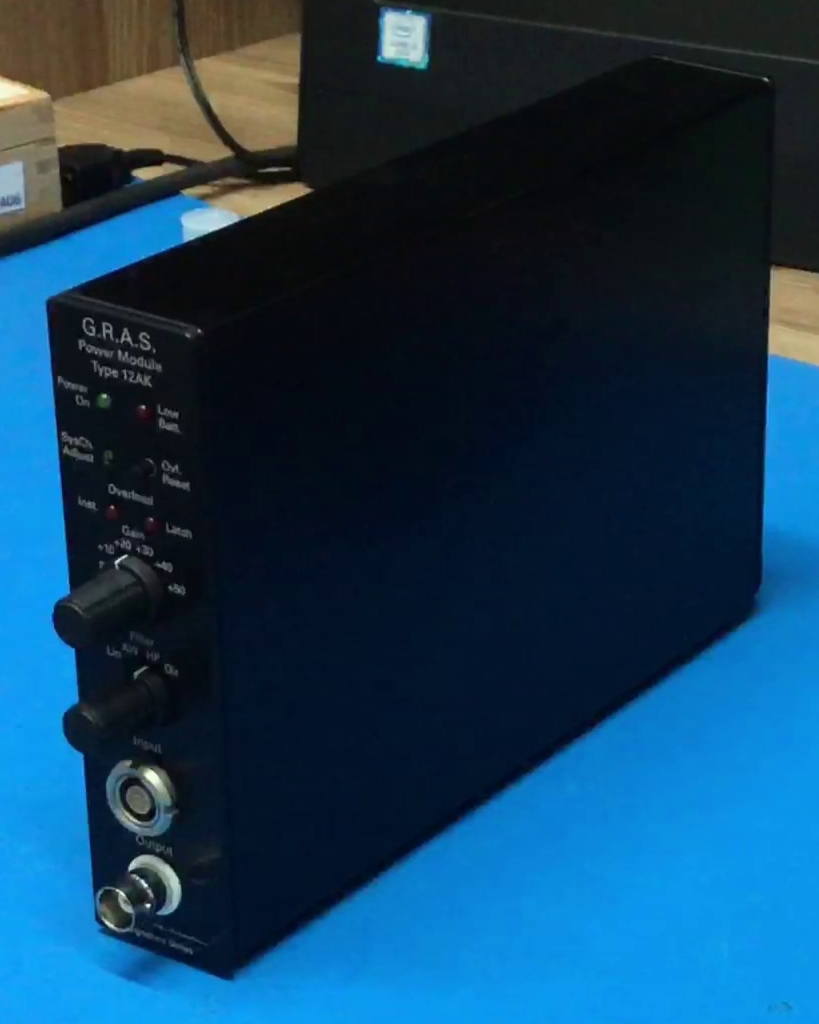
\includegraphics[height=7cm]{2_Metodología/Figs/gras12AK}
        \caption{Módulo de poder para preamplificadores y micrófonos GRAS 12AK.}
        \label{fig:gras_12AK}
    \end{subfigure}
\end{figure}

Como indica la norma \mbox{IEC 60942}~\citeyearpar{IEC_TC29_2017}, uno de los posibles métodos para calibrar calibradores acústicos es por comparación contra un calibrador patrón.\ Ese es el método elegido en este trabajo.
El calibrador acústico patrón elegido debe ser de las especificaciones más altas posibles, y su elección también determina el alcance de calibración del laboratorio.
Para este trabajo se emplea el calibrador Brüel \& Kjær 4231 (ver figura~\ref{fig:bruel_4231}), el cual es de clase LS y tiene disponibles dos niveles de presión sonora ($\qtylist{94;114}{\dB}$) a $\qty{1}{\kHz}$.
La trazabilidad de este calibrador se mantiene directamente con el fabricante.

El método requiere también un micrófono de referencia con el cuál se pueda transformar la señal acústica en una señal eléctrica para que pueda ser analizada posteriormente en amplitud, frecuencia y distorsión armónica más ruido (THD+N).
Se empleó el micrófono GRAS 40CE (ver figura~\ref{fig:gras_40CE}), el cual es un micrófono de campo libre con una sensibilidad típica de $\num{40}\,\nicefrac{\unit{\mV}}{\unit{\Pa}}$ y cuenta con su certificado de calibración de fábrica, en el que es posible determinar la diferencia entre las respuestas de campo libre y de campo de presión a $\qty{1}{\kHz}$.

La señal eléctrica del micrófono debe ser adecuada antes de medirla, por lo que se usa un preamplificador 01dB PRE22 (ver figura~\ref{fig:PRE22_01dB}).
Para polarizar el preamplificador se usa un módulo de poder GRAS 12AK (mostrado en la figura~\ref{fig:gras_12AK}), el cual también puede darle mayor ganancia a la señal para mejorar la relación señal a ruido, aplicarle un filtro paso alto para eliminar la interferencia de baja frecuencia y permite hacer el acople de impedancias apropiado para conectar la señal a la entrada de los instrumentos de medición.

\begin{figure}[!h]
    \caption{Instrumentos de medición para la calibración periódica de calibradores acústicos.}
    \centering
    \begin{subfigure}[t]{0.45\textwidth}
        \centering
        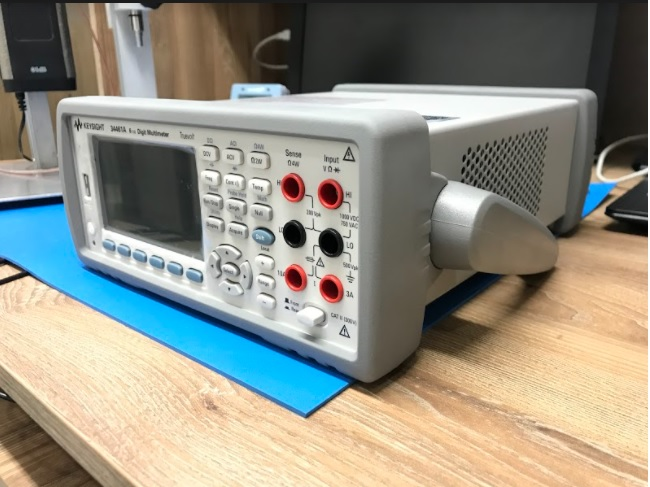
\includegraphics[height=6cm]{2_Metodología/Figs/keysight34461A}
        \caption{Multímetro digital Keysight 34461A.}
        \label{fig:keysight_34461A}
    \end{subfigure}
    \hfill
    \begin{subfigure}[t]{0.45\textwidth}
        \centering
        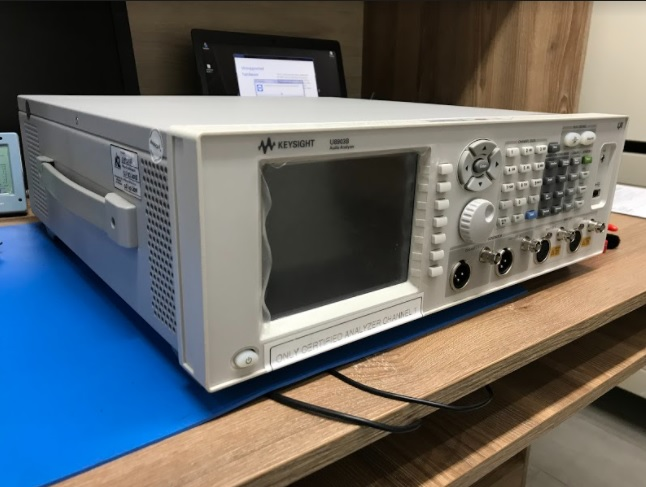
\includegraphics[height=6cm]{2_Metodología/Figs/keysightU8903B}
        \caption{Analizador de audio Keysight U8903B.}
        \label{fig:keysight_U8903B}
    \end{subfigure}
\end{figure}
%
Para medir el voltaje AC y la frecuencia se requiere un multímetro digital con suficientes dígitos de resolución que aporten la precisión requerida y no afecte negativamente la incertidumbre de medición.
El multímetro empleado es el Keysight 34461A de $6\nicefrac{1}{2}$ dígitos (mostrado en la figura~\ref{fig:keysight_34461A}), que, aunque su impacto es proporcional con la escala de medición, en $\unit{\dB}$ resulta ser despreciable.
En $\unit{\Hz}$, debido a la escala lineal, tendrá un impacto mayor, pero sigue siendo despreciable.
Cabe resaltar que, dependiendo de la escala, no todos los dígitos están disponibles en la pantalla del multímetro, pero sí pueden adquirirse todos siempre por la interfaz remota.
Este multímetro mantiene su trazabilidad a los patrones nacionales.

En cuanto a la THD+N, podría usarse una interfaz de sonido con un software de análisis en frecuencia, pero establecer su trazabilidad metrológica es poco factible.
Se requiere un instrumento que igualmente pueda ser calibrado por un laboratorio acreditado para esta magnitud (que es una magnitud bastante inusual).
Tal es el analizador de audio Keysight U8903B, que cuenta con una resolución de $7$ dígitos, disponibles completamente sólo mediante la interfaz remota.
Este instrumento cuenta con bastantes prestaciones especializadas para el análisis de audio.
Entre estas, unas importantes para los propósitos de este trabajo son: Establecer la impedancia de entrada, tipo de entrada (balanceada o no balanceada), desacople DC de la señal de entrada, filtros paso alto o paso bajo para la entrada, frecuencia de muestreo variable y cálculo de estadísticas en tiempo real.
Este analizador se muestra en la figura~\ref{fig:keysight_U8903B}.

Ambos instrumentos de Keysight cuentan con la interfaz de comunicación GPIB, mediante la cual estos pueden conectarse a un sólo puerto USB del computador para su control con instrucciones SCPI\@.

\subsection{Patrones e instrumentos para la calibración periódica de sonómetros}

\begin{figure}[!h]
    \caption{Esquema de conexiones de los instrumentos para la calibración periódica de sonómetros.}
    \label{fig:IEC61672_connections}
    \begin{subfigure}[t]{0.59\textwidth}
        \centering
        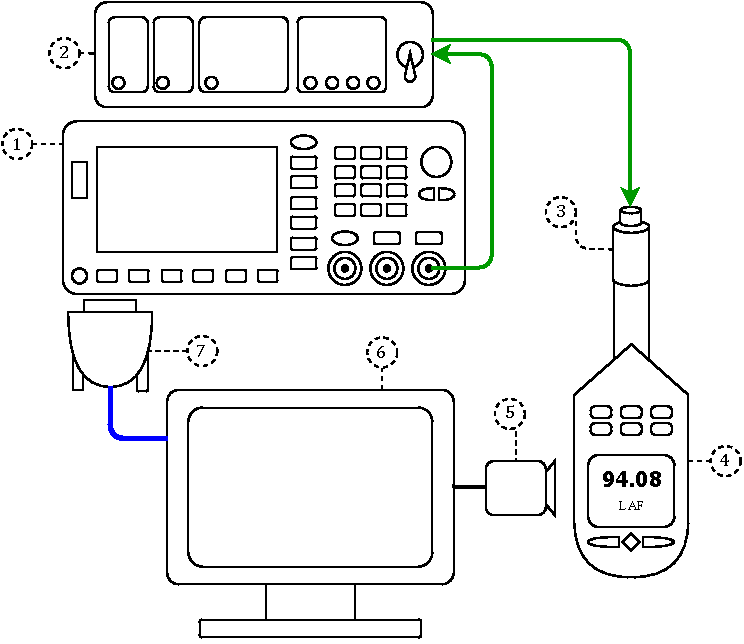
\includegraphics[width=0.95\textwidth]{2_Metodología/Figs/IEC61672-3connections}
    \end{subfigure}
    \hfill
    \begin{subfigure}[t]{0.4\textwidth}
        \centering
        \begin{tikzpicture}
            \node [draw]{\vbox{\scriptsize{
                \begin{enumerate}
                    \item Generador de señales Keysight 33511B
                    \item Atenuador programable ACOEM OUT-1694000
                    \item Adaptador de impedancia 01dB ADP12
                    \item Sonómetro
                    \item Cámara
                    \item Computador
                    \item Interfaz GPIB Keysight 82357B
                \end{enumerate}}
            \raggedright\qquad\textbf{\color{blue} —} Conexión GPIB \\
            \raggedright\qquad\textbf{\color{oliva_green} —} Conexión BNC}};
        \end{tikzpicture}
    \end{subfigure}
    \caption*{\footnotesize Fuente: Elaboración propia.}
\end{figure}

La interconexión propuesta para la calibración de sonómetros se presenta en la figura~\ref{fig:IEC61672_connections}.
A continuación se describe cada instrumento.
%
\clearpage

\begin{figure}[!h]
    \caption{Instrumentos utilizados en la calibración periódica de sonómetros.}
    \centering
    \begin{subfigure}[t]{0.49\textwidth}
        \centering
        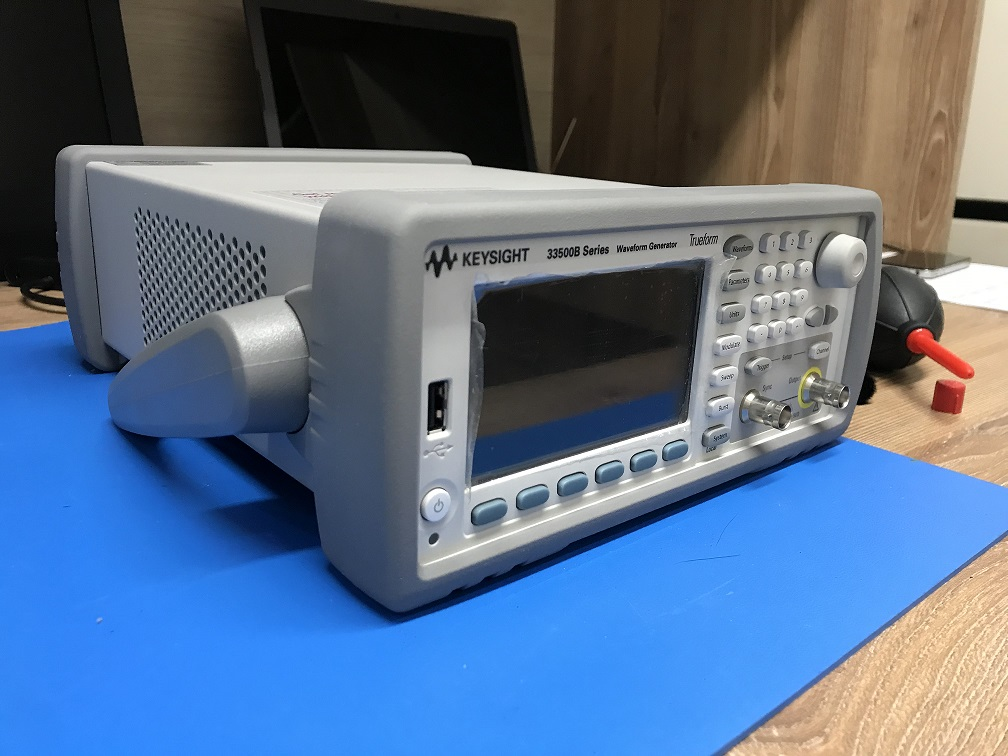
\includegraphics[height=6cm]{2_Metodología/Figs/keysight33511B}
        \caption{Generador de funciones arbitrarias Keysight 33511B.}
        \label{fig:keysight_33511B}
    \end{subfigure}
    \hfill
    \begin{subfigure}[t]{0.49\textwidth}
        \centering
        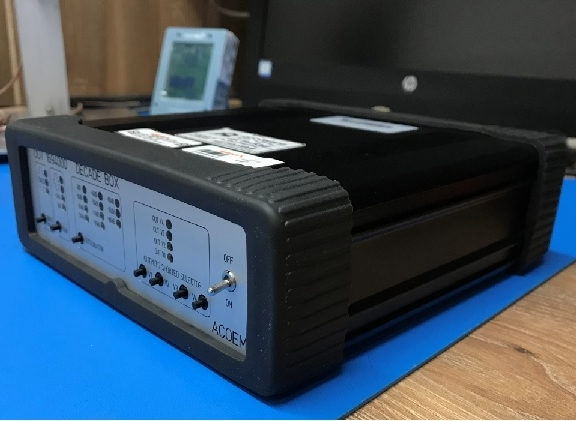
\includegraphics[height=6cm]{2_Metodología/Figs/decadebox}
        \caption{Atenuador programable ACOEM OUT-1694000.}
        \label{fig:decade_box}
    \end{subfigure}
\end{figure}
%
El flujo de señal inicia en el generador de señales.
En este trabajo se empleó el generador de funciones arbitrarias Keysight 33511B (véase figura~\ref{fig:keysight_33511B}), que tiene significativas prestaciones como la definición personalizada de formas de onda y un desempeño superior dada su baja distorsión armónica (típicamente $\num{0.04}\%$), amplio ancho de banda e intervalo de voltaje, bajo efecto de \emph{jitter}, su filtro \emph{anti-alias}, su resolución de amplitud de $\qty{16}{\bit}$ y de frecuencia de $\qty{1}{\micro\Hz}$, respuesta en frecuencia plana ($\pm\qty{0.10}{\dB}$ en todo el rango inferior a $\qty{100}{\kHz}$), alta precisión en amplitud ($\pm1\%$ del valor establecido $\pm\qty{1}{\mV}$) y en frecuencia ($\pm\qty{2}{ppm}$ del valor establecido $\pm\qty{15}{\pico\Hz}$).
El generador 33511B también cuenta con la interfaz de comunicación GPIB para su control remoto.
Este generador cumple la función de patrón de medición, generando señales eléctricas para \emph{simular} los niveles de presión sonora, y mantiene su trazabilidad a los patrones nacionales.

A pesar de que el generador tiene un rango de voltaje AC amplio ($\qty{1}{\mVpp}$ a $\qty{10}{\Vpp}$), para la mayoría de aplicaciones en sonómetros (cuyos micrófonos tienen sensibilidades típicas entre $\qtylist{40;50}{\mV}$), se requieren voltajes del orden de $\qty{13}{\Vrms}$ aproximadamente, con el fin de alcanzar los niveles más altos (cercanos a los $\qty{140}{\dB}$). Y para los niveles más bajos (cercanos a los $\qty{23}{\dB}$), se requieren voltajes del orden de $\qty{7}{\uVrms}$.
Por tal motivo se hace necesario un dispositivo adicional que amplifique la señal hasta al menos $\qty{6}{\dB}$ más y que sea capaz de atenuarla hasta al menos $\qty{50}{\dB}$.
Para esto se usó un \emph{Decade Box} o atenuador programable fabricado por ACOEM, el cual se muestra en la figura~\ref{fig:decade_box}.

Finalmente, el flujo de señal termina en el adaptador de impedancias.
Este debe ser preferiblemente el recomendado en el manual de instrucciones del sonómetro, o en su defecto debe usarse uno cuya capacitancia se equipare a la capacitancia del micrófono del sonómetro y que por supuesto tenga el mismo diámetro y rosca.
Como ejemplo, para sonómetros marca 01dB, se utiliza el adaptador 01dB ADP12, que se muestra en la figura~\ref{fig:PRE22_01dB}.

Adicionalmente, para capturar el valor de medición indicado en la pantalla del sonómetro, se usa una cámara web conectada al computador.

\subsection{Comandos SCPI}
\label{subsec:scpi_commands}
En esta sección se explica de forma general el protocolo de comandos estándar para instrumentos programables (SCPI), tomando como guía de referencia el manual del generador Keysight 33511B~\citeyearpar{Keysight2015}.

Los comandos SCPI son un lenguaje basado en ASCII para instrumentos de medición y de pruebas.
Estos comandos están basados en una estructura jerárquica conocida como sistema de árbol, en el que los comandos asociados están agrupados bajo un nodo o raíz común, formando así los subsistemas.
Por ejemplo, una parte de la estructura del sistema \texttt{\small OUTPut} es la siguiente:
%
\begin{Verbatim}[fontsize=\footnotesize]
OUTPut:
    SYNC {OFF|0|ON|1}
    SYNC:
        MODE {NORMal|CARRier}
        POLarity {NORMal|INVerted}
\end{Verbatim}

Las líneas sin sangría son los sistemas raíces y cada nivel de sangría corresponde al nivel del subsistema en la jerarquía.
El ``\textbf{:}" separa una palabra clave de otra en un nivel más bajo.
Las letras en mayúsculas son abreviaciones de las palabras clave de los comandos, que también pueden ser usadas opcionalmente, quitando las letras en minúsculas de la palabra clave.
Las llaves (\textbf{\{\}}), en realidad indican que se esperan los parámetros para un comando dado, los cuales pueden tomar valores numéricos, booleanos, cadenas de texto o palabras clave que denotan valores preestablecidos.
Si un comando espera más de un parámetro, estos son separados por comas.
Por ejemplo, para habilitar la salida del generador ajustándolo en una forma de onda senoidal de $\qty{1}{\kHz}$, con una amplitud de $\qty{50}{\mV}$ y un \emph{offset} DC de $\qty{0}{\V}$, se enviaría el siguiente comando: \texttt{\small APPL:SIN 1E3,50E-3,0.0}.

También se puede reducir la extensión de los códigos usando ``\textbf{;}" para separar instrucciones de un mismo sistema de mayor nivel.
Por ejemplo, la instrucción \texttt{\small TRIG:SOUR BUS; COUNT 30} logra el mismo efecto que las instrucciones \texttt{\small TRIG:SOUR BUS} y \texttt{\small TRIG:COUNT 30} enviadas una tras otra.

Se puede consultar el valor actual de la mayoría de parámetros de sistemas o subsistemas usando ``\textbf{?}". Por ejemplo, con el comando \texttt{\small :CALC:STAT:DATA1?} se obtiene el primer valor estadístico calculado por el analizador de audio, según se haya configurado previamente.

Cada instrumento de Keysight usado en este trabajo cuenta con un conjunto específico de sistemas y subsistemas para realizar las funciones particulares según su naturaleza, los cuales pueden ser consultados en las guías de referencia de comandos SCPI de los respectivos manuales o, de una forma mucho más interactiva, en la aplicación \emph{Command Expert} de Keysight.
También hay comandos comunes a la mayoría de instrumentos como los siguientes: \texttt{\small *IDN?} (consulta la información de identificación del instrumento) y \texttt{\small *TST?} (ejecuta la secuencia de autoverificación del instrumento).

El control remoto de los instrumentos con comandos SCPI se implementó en Python con la librería \texttt{\small PyVisa}~\citeyearpar{PyVisa2022}, la cual requiere que en el computador esté instalada por lo menos la librería VISA de \emph{National Instruments} o, como en este desarrollo, la \emph{Keysight IO Library Suite} \citepalias{Keysight2022}, las cuales son totalmente gratuitas.

%  ╦═╗┌─┐┌─┐┌─┐┌┐┌┌─┐┌─┐┬┌┬┐┬┌─┐┌┐┌┌┬┐┌─┐  ┌┬┐┌─┐  ┬┌┬┐┌─┐┌─┐┌─┐┌┐┌┌─┐┌─┐
%  ╠╦╝├┤ │  │ │││││ ││  │││││├┤ │││ │ │ │   ││├┤   ││││├─┤│ ┬├┤ │││├┤ └─┐
%  ╩╚═└─┘└─┘└─┘┘└┘└─┘└─┘┴┴ ┴┴└─┘┘└┘ ┴ └─┘  ─┴┘└─┘  ┴┴ ┴┴ ┴└─┘└─┘┘└┘└─┘└─┘

\chapter{Sistema de reconocimiento de imágenes para el valor de medición}
\label{ch:image_recognition}
En esta sección se discute el desarrollo del sistema de reconocimiento de caracteres que será empleado para adquirir automáticamente un valor de medición que sea indicado en la pantalla del sonómetro bajo calibración.
Primero se introduce un algoritmo general con los pasos de procesamiento y clasificación de las imágenes;
luego, se presenta el fundamento teórico de cada uno de esos pasos.
Finalmente, se muestran y discuten los resultados de procesamiento de imagen sobre una muestra de un dígito, como también los resultados del clasificador implementado.

\section*{Algoritmo de reconocimiento de caracteres}
De manera general, la solución propuesta, para el reconocimiento del valor de medición indicado en la pantalla del sonómetro, consta de varios pasos que se presentan en el siguiente algoritmo.

\begin{algorithm}[H]
    \caption{Algoritmo del sistema de reconocimiento de imágenes.}
    \label{alg:image_recongnition}
    \scriptsize
    \DontPrintSemicolon
    \SetKwData{image}{image} \SetKwData{images}{images} \SetKwData{training}{training} \SetKwData{features}{features} \SetKwInOut{Output}{output}
    \KwData{\images $\leftarrow$ \text{Imágenes de entrenamiento si va a entrenar o fotos de la pantalla si va reconocer.}}
    \Output{Clases estimadas.}
    \BlankLine
    \training $\leftarrow$ \emph{True} $|$ \emph{False}\;
    \ForEach{\image $\in$ \images}{
        \textbackslash\textbackslash Las operaciones sobre \image son realizadas \emph{in place}.\;
        \textbf{\hyperref[sec:gaussian_filter]{Paso 1}:} Filtrar \image con filtro gaussiano.\;
        \textbf{\hyperref[sec:padding]{Paso 2}:} Escalar y hacer \emph{padding} a \image para hacerla de $31 \times 32$ píxeles.\;
        \textbf{\hyperref[sec:segmentation]{Paso 3}:} Segmentar \image determinando el umbral con el método de \citet{Otsu1979}.\;
        \If{\training $=$ False}{
            Detectar contornos y extraer dígitos.\;
        }
        \textbf{\hyperref[sec:sift_descriptor]{Paso 4}:} Calcular las características de \image con el descriptor SIFT~\citep{Lowe2004}.\;
        \textbf{\hyperref[sec:kpca_reduction]{Paso 5}:} Reducir dimensionalidad de las características por KPCA~\citep{Scholkopf1997}.\;
        Agregar las características a la matriz \features.\;
    }
    \textbf{\hyperref[sec:nb_classifier]{Paso 6}:}\;
    \eIf{\training}{
        Entrenar clasificador bayesiano normal con \features y las correspondientes etiquetas de clase.\;}
    {
        Estimar las clases de las características en \features con el clasificador bayesiano normal.\;}
\end{algorithm}

%\begin{figure}
%	\caption{Diagrama de flujo del algoritmo de reconocimiento de caracteres}
%	\label{fig:flowchart}
%	\centering
%	\begin{tikzpicture}[font=\scriptsize, node distance=1.5cm]
%		\node (start1) at (-6, 5) [draw, terminal, minimum width=2cm, minimum height=0.5cm] {Inicio};
%		\node (subrutine1) [draw, predproc, minimum width=2cm, align=center,
%							minimum height=0.5cm, below of=start1] {Entrenar \\ clasificador};
%		\node (process1) [draw, process, minimum width=2cm, align=center,
%						  minimum height=0.5cm, below of=subrutine1] {Configurar \\ multímetro};
%		\node (subrutine2) [draw, predproc, minimum width=2cm, align=center,
%							minimum height=0.5cm, below of=process1] {Detección del \\ área de interés (ROI)};
%		\node (process2) [draw, process, minimum width=2cm, align=center,
%						  minimum height=0.5cm, below of=subrutine2] {Enviar señal \\ de prueba};
%		\node (process2_north) [draw, circle, fill=black, inner sep=0pt,
%								minimum size=2pt, above of=process2, node distance=0.75cm] {};
%		\node (subrutine3) [draw, predproc, minimum width=2cm, align=center,
%							minimum height=0.5cm, below of=process2] {Reconocimiento \\ del resultado};
%		\node (storage1) [draw, storage, minimum width=2cm, align=center,
%						  minimum height=0.5cm, below of=subrutine3] {Almacenar \\ resultado};
%		\node (decide1) [draw, conditional, minimum width=2cm,
%						 minimum height=0.5cm, below of=storage1] {¿Prueba finalizada?};
%		\node (decide1_east) [right of=decide1, node distance=3cm]{};
%		\node (print1) [draw, print, minimum width=2cm, align=center,
%						minimum height=0.5cm, below of=decide1] {Presentar \\ resultados};
%		\node (finish1) [draw, terminal, minimum width=2cm, minimum height=0.5cm, below of=print1] {Fin};
%
%		\draw [arrow] (start1) -- (subrutine1);
%		\draw [arrow] (subrutine1) -- (process1);
%		\draw [arrow] (process1) -- (subrutine2);
%		\draw [arrow] (subrutine2) -- (process2);
%		\draw [arrow] (process2) -- (subrutine3);
%		\draw [arrow] (subrutine3) -- (storage1);
%		\draw [arrow] (storage1) -- (decide1);
%		\draw [thick] (decide1) -- node[pos=0.1, above]{No} (decide1_east.center);
%		\draw [arrow] (decide1_east.center) |- (process2_north);
%		\draw [arrow] (decide1) -- node[right] {Sí} (print1);
%		\draw [arrow] (print1) -- (finish1);
%		
%		\node (start2) at (0, 5) [draw, terminal, minimum width=2cm,
%								  align=center, minimum height=0.5cm] {Entrenar \\ clasificador};
%		\node (process3) [draw, process, minimum width=2cm, minimum height=0.5cm,
%						  align=center, below of=start2] {Filtro \\ gaussiano};
%		\node (database1) [minimum width=2cm, right of=start2,
%						  node distance = 3 cm, align=center] {Imágenes de \\ entrenamiento};
%		\draw (database1.north west) -- (database1.south west)
%			  .. controls +(-30:0.2cm) and +(-150:0.2cm) .. (database1.south east)
%			  -- (database1.north east) .. controls +(-150:0.2cm) and +(-30: 0.2cm) .. (database1.north west)
%			  -- +(0, 0.2cm) .. controls +(-30:0.2cm) and +(-150:0.2cm) .. +(2.01cm, 0.2cm)
%			  .. controls +(150:0.2cm) and +(30:0.2cm) .. +(0,0.2cm) -- +(0, 0.1cm)
%			  .. controls +(-30:0.2cm) and +(-150:0.2cm) .. +(2.01cm, 0.1cm)
%			  -- (database1.north east) -- +(0cm, 0.2cm);
%		\node (process4) [draw, process, minimum width=2cm, align=center,
%						  minimum height=0.5cm, below of=process3] {Escalización \\ y \emph{padding}};
%		\node (process5) [draw, process, minimum width=2cm, minimum height=0.5cm, below of=process4] {Binarización};
%		\node (process6) [draw, process, minimum width=2cm, align=center,
%						  minimum height=0.5cm, below of=process5] {Cálculo del \\ descriptor SIFT};
%		\node (process7) [draw, process, minimum width=2cm, align=center,
%						  minimum height=0.5cm, below of=process6] {Reducción de \\ dimensionalidad con \\ KPCA};
%		\node (process8) [draw, process, minimum width=2cm, align=center,
%						  minimum height=0.5cm, below of=process7] {Ajuste del clasificador \\ normal bayessiano};
%		\node (finish2) [draw, terminal, minimum width=2cm, minimum height=0.5cm, below of=process8] {Volver};
%		
%		\draw [arrow] (start2) -- (process3);
%		\draw [thick, <-, stealth-] (process3.east) -| ++(2cm, 1.08cm);
%		\draw [arrow] (process3) -- (process4);
%		\draw [arrow] (process4) -- (process5);
%		\draw [arrow] (process5) -- (process6);
%		\draw [arrow] (process6) -- (process7);
%		\draw [arrow] (process7) -- (process8);
%		\draw [arrow] (process8) -- (finish2);
%		
%		\node (start3) at (7, 5) [draw, terminal, align=center,
%		minimum width=2cm, minimum height=0.5cm] {Reconocimiento \\ del resultado};
%		\node (process9) [draw, process, align=center, below of=start3,
%		            minimum width=2cm, minimum height=0.5cm,
%		            node distance=1.2cm] {Capturar imagen y \\ extraer región de interés};
%	    \node (process10) [draw, process, below of=process9, minimum width=2cm,
%	    				   minimum height=0.5cm, node distance=1.2cm] {Filtro gaussiano};
%	    \node (process11) [draw, process, below of=process10, align=center,
%	    				   minimum width=2cm, minimum height=0.5cm, node distance=1.2cm] {Escalización \\ y \emph{padding}};
%	    \node (process12) [draw, process, below of=process11, minimum width=2cm,
%	    				   minimum height=0.5cm, node distance=1.2cm] {Binarización};
%	    \node (process13) [draw, process, align=center, below of=process12, minimum width=2cm,
%	    				   minimum height=0.5cm, node distance=1.2cm] {Detección de contornos \\ y extracción de dígitos};
%	    \node (process14) [draw, process, align=center, below of=process13, minimum width=2cm,
%	    				   minimum height=0.5cm, node distance=1.5cm] {Cálculo del \\ descriptor SIFT};
%	    \node(process15) [draw, process, align=center, below of=process14, minimum width=2cm,
%	    				  minimum height=0.5cm, node distance=1.5cm] {Reducción de \\ dimensionalidad con \\ KPCA};
%	    \node(process16) [draw, process, align=center, below of=process15, minimum width=2cm,
%	    				  minimum height=0.5cm, node distance=1.5cm] {Clasificación \\ del caracter};
%	    \node (print2) [draw, print, align=center, below of=process16, minimum width=2cm,
%	    				minimum height=0.5cm, node distance=1.2cm] {Resultado \\ numérico};
%	    \node (finish3) [draw, terminal, below of=print2, minimum width=2cm,
%	    				 minimum height=0.5cm, node distance=1.2cm] {Volver};
%	    
%	    \draw [arrow] (start3) -- (process9);
%	    \draw [arrow] (process9) -- (process10);
%	    \draw [arrow] (process10) -- (process11);
%	    \draw [arrow] (process11) -- (process12);
%	    \draw [arrow] (process12) -- (process13);
%	    \draw [arrow] (process13) -- (process14);
%	    \draw [arrow] (process14) -- (process15);
%	    \draw [arrow] (process15) -- (process16);
%	    \draw [arrow] (process16) -- (print2);
%	    \draw [arrow] (print2) -- (finish3);
%	\end{tikzpicture}
%\end{figure}

Concerniente al procesamiento y reconocimiento de imágenes, a continuación se presenta un breve marco de referencia teórico de cada paso del algoritmo~\ref{alg:image_recongnition}.

\section*{Paso 1: Filtro gaussiano}
\label{sec:gaussian_filter}
Como se explica en el libro de Robert Szeliski~\citeyearpar{Richard2011}, el filtro gaussiano, también llamado filtro de suavizado o de desenfoque, es una operación local en imágenes bidimensionales, pues se efectúa en vecindarios con un tamaño determinado en píxeles;
el valor final de un píxel depende de los valores de los píxeles que pertenecen a su correspondiente vecindario y, como en todos los casos de filtros lineales, de una función de ponderación.
Esta operación local viene a ser la de correlación $\left(g = f \otimes h\right)$, que básicamente es la suma ponderada de los píxeles de entrada, que se define como
%
\begin{equation}
    \label{eq:correlation}
    g(i, j) = \sum_{k, l} f(i + k, j + l)\,h(k, l).
\end{equation}
%
En que $g$ es la imagen de salida, $f$ es la imagen de entrada y $h$ la máscara o \emph{kernel}, que contiene los coeficientes del filtro.

La operación contraparte de la correlación sería la convolución $\left(g = f \ast h\right)$, en la que se usa el \emph{kernel} invertido y se define como
%
\begin{equation}
    \label{eq:convolution}
    g(i, j) = \sum_{k, l} f(k, l)\,h(i - k, j - l).
\end{equation}
%
En que $h$ es la respuesta al impulso, ya que si se convoluciona la máscara $h$ con una señal impulsiva $\delta(i, j)$, se obtiene la misma máscara $\left(h \ast \delta = h\right)$.

Para el caso del filtro gaussiano, el \emph{kernel} se obtiene a partir de la típica función exponencial de Gauss.
Particularmente, considerando la implementación de \texttt{\small OpenCV} que se ejecuta con la instrucción \texttt{\small GaussianBlur()}, la función sería la bivariada no correlacionada definida como
%
\begin{equation}
    \label{eq:bivariate_gaussian}
    h(x, y) = \frac{1}{2\pi\sigma_x\sigma_y}
    \exp\left(-\frac{\left(x - \mu_x\right)^2}{2\sigma_x^2} - \frac{\left(y - \mu_y\right)^2}{2\sigma_y^2}\right).
\end{equation}

La función de \texttt{\small OpenCV} también permite especificar un tamaño definido de ventana y esta calculará automáticamente las varianzas como
%
\begin{subequations}
    \label{eq:variance_from_kernel}
    \begin{align}
        \sigma_x &= \left(\frac{n_x - 1}{2}\right)\,0.3 + 0.8, \quad \text{en que } n_x = \text{ancho} - 1; \label{eq:variance_from_kernel_1} \\
        \sigma_y &= \left(\frac{n_y - 1}{2}\right)\,0.3 + 0.8, \quad \text{en que } n_y = \text{alto} - 1. \label{eq:variance_from_kernel_2}
    \end{align}
\end{subequations}

\section*{Paso 2: Escalización y \emph{padding}}
\label{sec:padding}
Por supuesto, en la práctica, el filtrado requiere que se agreguen píxeles en los bordes de la imagen original, según el tamaño determinado de la ventana;
a esto se le conoce como \emph{padding} y es una operación que realiza por defecto \texttt{\small OpenCV}, con la que es posible elegir el modo del \emph{padding}.
Existen diferentes modos de \emph{padding}, de los cuales se describen los siguientes:
%
\begin{itemize}
    \item \emph{zero}: Todos los píxeles añadidos se establecen en $0$.
    \item \emph{mirror}: Refleja los últimos pixeles del borde.
\end{itemize}

En la siguiente figura se muestra el resultado de ambos modos de \emph{padding}.
%
\begin{figure}[h!]
    \caption{Comparación de los modos de \emph{padding}: \emph{zero} y \emph{mirror}.}
    \label{fig:padding_comparison}
    \centering
    \begin{subfigure}[t]{0.3\textwidth}
        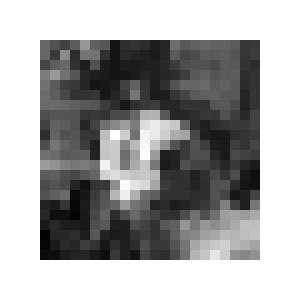
\includegraphics[width=\textwidth]{3_Reconocimiento/Figs/for_padding}
        \caption{Imagen original}
    \end{subfigure}
    \hfill
    \begin{subfigure}[t]{0.3\textwidth}
        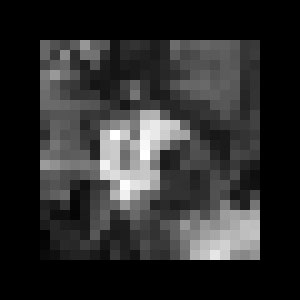
\includegraphics[width=\textwidth]{3_Reconocimiento/Figs/zero_padding}
        \caption{\emph{zero padding}}
    \end{subfigure}
    \hfill
    \begin{subfigure}[t]{0.3\textwidth}
        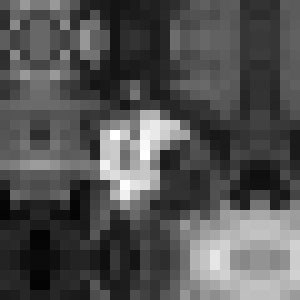
\includegraphics[width=\textwidth]{3_Reconocimiento/Figs/mirror_padding}
        \caption{\emph{mirror padding}}
    \end{subfigure}
    \caption*{\footnotesize Tomado de~\citep{Richard2011}.}
\end{figure}

El modo \emph{mirror} es utilizado para el filtro gaussiano y el \emph{zero} para adecuar la imagen antes del \hyperref[sec:segmentation]{paso 3} con el fin de completar el tamaño de $32 \times 32$ píxeles requerido para el \hyperref[sec:sift_descriptor]{paso 4}.

Como la imagen que contiene el dígito tendrá un tamaño diferente a $32 \times 32$, antes de efectuar el \emph{zero padding}, es necesario escalarla haciendo que el eje de mayor dimensión se ajuste a $32$ píxeles y el otro eje se ajuste proporcionalmente;
esta operación se lleva a cabo con la función \texttt{\small resize()} de \texttt{\small OpenCV}.
Luego sí se añaden los píxeles faltantes al eje de menor dimensión para completar los $32$ píxeles.
\vfill

\section*{Paso 3: Segmentación}
\label{sec:segmentation}
Existen diferentes técnicas de segmentación: basada en umbrales, en bordes, en regiones, por agrupación o por \emph{matching}.
Para los propósitos de este trabajo, es suficiente con una umbralización para discriminar los segmentos de la imagen, que corresponderían a los dígitos indicados en la pantalla del sonómetro.
Sin embargo, el umbral no puede ser el mismo para todas las imágenes, pues cada una puede estar influenciada por los efectos de iluminación, áreas o colores de los segmentos.
Una forma sistemática de determinar el umbral es empleando el algoritmo de \citet{Otsu1979}.
Este algoritmo busca maximizar la separación entre las clases de niveles de grises del histograma de la imagen usando los momentos de cero y primer orden.

La formulación de Otsu es un \emph{método no supervisado}\footnote{Los métodos no supervisados son aquellos que no requieren que las muestras de entrenamiento estén etiquetadas previamente según su clase, sino que a partir de los datos identifican patrones que permiten agruparlos.} basado en el análisis discriminante para evaluar la bondad del umbral y seleccionar automáticamente un límite óptimo.
En primer lugar, el método normaliza el histograma de niveles de grises y lo considera como una distribución de probabilidad.

Si hay $L$ niveles de grises, entonces el número de píxeles en la imagen es $N = n_1 + n_2 + \cdots + n_L$; $n_i$ es el número de píxeles que tienen un nivel $i$.
Luego, la distribución de probabilidad queda expresada como
%
\begin{equation}
    \label{eq:hist_p_distribution}
    p_i = \frac{n_i}{N}, \quad \text{en que } p_i \geq 0, \sum_{i = 1}^L p_i = 1.
\end{equation}

Ahora, se buscan dos clases $C_0$ y $C_1$, que corresponden a los píxeles que pertenecen al fondo y a los que pertenecen a los objetos, separados por el nivel de gris de valor $k$.
Las probabilidades de cada clase se definen de acuerdo con
%
\begin{subequations}
    \label{eq:otsu_class_probs}
    \begin{align}
        \omega_0 &= \mathrm{Pr}\left(C_0\right) = \sum_{i = 1}^k p_i = \omega(k); \label{eq:otsu_class_probs_1} \\
        \omega_1 &= \mathrm{Pr}\left(C_1\right) = 1 - \omega(k). \label{eq:otsu_class_probs2}
    \end{align}
\end{subequations}
%
Luego, los valores esperados condicionales de cada clase son:
%
\begin{subequations}
    \label{eq:otsu_expected_values}
    \begin{align}
        \mu_0 &= \sum_{i = 1}^k i\,\mathrm{Pr}\left(i|C_0\right) =
        \sum_{i = 1}^k i\,\frac{p_i}{\omega_0} = \frac{\mu(k)}{\omega(k)}; \label{eq:otsu_expected_values_1} \\
        \mu_1 &= \sum_{i = k + 1}^L i\,\mathrm{Pr}\left(i|C_i\right) =
        \sum_{i = k + 1}^L i\,\frac{p_i}{\omega_1} =
        \frac{\mu_T - \mu(k)}{1 - \omega(k)}. \label{eq:otsu_expected_values_2}
    \end{align}
\end{subequations}
%
En que $\omega(k)$ y $\mu(k)$ son los momentos acumulados de cero y primer orden del histograma hasta el $k$-ésimo nivel.
Estos momentos acumulados se definen como
%
\begin{subequations}
    \label{eq:otsu_cumulative_moments}
    \begin{align}
        \omega(k) &= \sum_{i = 1}^k p_i; \label{eq:otsu_cumulative_moments_1} \\
        \mu(k) &= \sum_{i = 1}^k i\,p_i.\label{eq:otsu_cumulative_moments_2}
    \end{align}
\end{subequations}

Similarmente, los momentos de primer y segundo orden de la imagen se definen como
%
\begin{subequations}
    \label{eq:otsu_total_moments}
    \begin{align}
        \mu_T &= \sum_{i = 1}^L i\,p_i; \label{eq:otsu_total_moments_1} \\
        \sigma_T^2 &= \sum_{i = 1}^L \left(i - \mu_T\right)^2\,p_i. \label{eq:otsu_total_moments_2}
    \end{align}
\end{subequations}
%
En que $\mu_T$ es la media total de los niveles de grises de la imagen original y $\sigma_T^2$ la varianza.

En principio, si las clases están separadas en sus niveles de grises entonces hay una umbralización adecuada.
Consecuentemente, un umbral que resulte en la mejor separación de clases según sus niveles de grises será un umbral óptimo.
Hay por lo menos tres medidas de separación entre clases que se pueden maximizar.
Sin embargo, por simplicidad (dado que depende de los momentos de orden cero y uno), conviene usar la medida definida en la siguiente ecuación como criterio para el análisis discriminante.
%
\begin{equation}
    \eta = \frac{\sigma_B^2}{\sigma_T^2}. \label{eq:otsu_discriminant_criterion}
\end{equation}
%
Donde el coeficiente $\sigma_B^2$ se define como
%
\begin{equation}
    \sigma_B^2 = \omega_0\,\omega_1\,\left(\mu_1 - \mu_0\right)^2. \label{eq:otsu_between_variance}
\end{equation}

Finalmente, condensando las ecuaciones (\ref{eq:otsu_expected_values}) a~\eqref{eq:otsu_between_variance}, el umbral óptimo $k^*$ que maximiza $\eta$ y, proporcionalmente, $\sigma_B^2$ se encuentra por medio de la siguiente expresión:
%
\begin{equation}
    \sigma_B^2(k^*) = \max_{1 \le k < L} \sigma_B^2(k). \label{eq:otsu_optimum_threshold}
\end{equation}
%
En la cual,
%
\begin{equation}
    \sigma_B^2(k) = \frac{\left[\mu_T\,\omega(k) - \mu(k)\right]^2}
    {\omega(k)\,\left[1 - \omega(k)\right]}. \label{eq:otsu_between_variance4optimize}
\end{equation}

Esta optimización se puede realizar de forma iterativa con unos valores iniciales de $\omega(0)$ y $\mu(0)$, luego iterando con todos los posibles valores de $k = 0, 1, \cdots, L$, y calculando $\sigma_B^2(k)$.
El umbral óptimo $k^*$ será el máximo valor obtenido de $\sigma_B^2(k)$.


\section*{Paso 4: Descriptor local SIFT}
\label{sec:sift_descriptor}
En esta aplicación particular (cuyo funcionamiento se pretende en tiempo real), el objeto de reconocimiento es simple, por lo que no hace falta el sofisticado algoritmo de detección, localización y orientación de puntos característicos de la presentación original del descriptor SIFT propuesto por \citet{Lowe2004}.
No obstante, la implementación del algoritmo aquí presentada sí tiene en cuenta su propuesta de descriptor local basada en la magnitud y dirección de los gradientes de cada píxel perteneciente a la región alrededor de cada punto característico.

En primer lugar, se calcula la magnitud y dirección del gradiente de cada píxel.
Esto finalmente es una valoración del cambio direccional en la intensidad de la imagen.
La dirección final del gradiente en un píxel es aquella en la que ocurre el máximo cambio de intensidad, y la magnitud sería el máximo cambio de intensidad.
Para lo cual se emplean las siguientes ecuaciones:
%
\begin{subequations}
    \label{eq:sift_gradient}
    \begin{align}
        \delta_x &= I(x + 1, y) - I(x - 1, y); \label{eq:sift_gradient_1} \\
        \delta_y &= I(x, y + 1) - I(x, y - 1); \label{eq:sift_gradient_2} \\
        \theta(x,y) &= \tan^{-1}\left(\frac{\delta_y}{\delta_x}\right); \label{eq:sift_gradient_3} \\
        |\nabla f(x, y)| &= \sqrt{\delta_x^2 + \delta_y^2}. \label{eq:sift_gradient_4}
    \end{align}
\end{subequations}

Las diferencias de intensidad en $x$ y en $y$ se determinan con las ecuaciones~\eqref{eq:sift_gradient_1} y~\eqref{eq:sift_gradient_2}, luego, la dirección con~\eqref{eq:sift_gradient_3} y la magnitud con~\eqref{eq:sift_gradient_4}.

Después de obtener todas las magnitudes y direcciones de los gradientes, se conforma un histograma de orientaciones en $8$ intervalos por cada ventana de $n \times n = 4 \times 4$ píxeles;
es decir, según la dirección de cada vector, su magnitud se suma en el respectivo intervalo del histograma de la ventana al que pertenece.
Finalmente, queda un vector de características de $128$ valores que es la concatenación de todos los histogramas, cada uno de $8$ valores.
Pero la contribución de esta magnitud a su intervalo de orientación correspondiente es ponderada por la función gaussiana de la ecuación~\eqref{eq:sift_gaussian_weighting} con $\sigma$ igual a la mitad del ancho de la ventana del descriptor, con el propósito de dar menor peso a los gradientes que están más lejos del centro del descriptor.
%
\begin{equation}
    \label{eq:sift_gaussian_weighting}
    G(x,y) = \frac{1}{2\,\pi\,\sigma^2}\,\exp{\left(-\frac{x^2 + y^2}{2\,\sigma^2}\right)  }.
\end{equation}

El objetivo del histograma es permitir que haya cambios locales más grandes en las direcciones de los gradientes, pero que contribuyan al mismo intervalo en el histograma.
Ahora bien, pueden ocurrir cambios abruptos en el histograma cuando en realidad hay cambios suaves en las direcciones de las muestras de gradientes, esto debido a los efectos de los límites en los intervalos.
Para mitigar este efecto, se aplica una interpolación trilineal\footnote{La interpolación trilineal es la extensión de la interpolación lineal a un espacio tridimensional ($D = 3$) usando polinomios de primer orden. En la práctica resulta ser la interpolación lineal de dos interpolaciones bilineales. Con esta operación se encuentra un valor intermedio teniendo en cuenta los $2^D$ valores adyacentes.} para distribuir la magnitud de cada muestra de gradiente en intervalos de histograma adyacentes, en función de la ``distancia'' de la dirección de la muestra desde el valor central del intervalo.
Esto queda reflejado en las siguientes funciones de ponderación:
%
\begin{subequations}
    \begin{align}
        w_k(x, y) &= \left\{\begin{matrix}
                                \nabla\theta(x, y),     & \text{si } k = i\theta(x, y)       \\
                                1 - \nabla\theta(x, y), & \text{si } k = i\theta \bmod 8 + 1 \\
                                0,                      & \text{en caso contrario}
        \end{matrix} \right. \label{eq:sift_trilineal_weighting_1} \\
        w_i(x, y) &= \left\{\begin{matrix}
                                \nabla x(x, y),     & \text{si } i = ix(x, y)     \\
                                1 - \nabla x(x, y), & \text{si } i = ix(x, y) + 1 \\
                                0,                  & \text{en caso contrario}
        \end{matrix} \right. \label{eq:sift_trilineal_weighting_2} \\
        w_j(x, y) &= \left\{\begin{matrix}
                                \nabla y(x, y),     & \text{si } j = iy(x, y)     \\
                                1 - \nabla y(x, y), & \text{si } j = iy(x, y) + 1 \\
                                0,                  & \text{en caso contrario}
        \end{matrix} \right. \label{eq:sift_trilineal_weighting_3}
    \end{align}
\end{subequations}
%
Con las siguientes definiciones:
\begin{subequations}
    \begin{align}
        \nabla\theta(x, y) &= i\theta(x, y) - \frac{\theta(x, y)}{\delta\theta}, \quad \text{en que }
        i\theta(x, y) = \left\lceil \frac{\theta(x, y)}{\delta\theta} \right\rceil \text{y } \delta\theta = 360 / n; \\
        \nabla x(x, y) &= ix(x, y) - \frac{x}{\delta x}, \quad \text{en que } ix(x, y) = \left\lceil \frac{x}{\delta x} \right\rceil; \\
        \nabla y(x, y) &= iy(x, y) - \frac{y}{\delta x}, \quad \text{en que } iy(x, y) = \left\lceil \frac{y}{\delta x} \right\rceil.
    \end{align}
\end{subequations}

En seguida, se conforma el histograma como se presenta a continuación:
%
\begin{align}
    H &= \left(H_{11}, H_{12}, \cdots, H_{nn} \right); \nonumber \\
    H_j &= \left(h_1, h_2, \cdots, h_n\right); \nonumber \\
    h_{k}(x, y) &=
    \sum_{(x, y)} w_k(x, y)\,w_i(x, y)\,w_j(x, y)\,|\nabla f(x, y)|\,G(x, y).
\end{align}

Finalmente el arreglo resultante se normaliza para hacerlo invariante a los efectos de contrastes o cambios en la iluminación, y para reducir los efectos de cambios no lineales en iluminación debidos a la saturación de la cámara, se limitan los valores con un umbral experimental de $\num{0.2}$, de manera que los valores inferiores a $\num{0.2}$ son remplazados con $\num{0.2}$, y se normaliza nuevamente.
La normalización se efectúa empleando la norma $L_2$, como se muestra a continuación:
%
\begin{subequations}
    \begin{align*}
        H &= \left(H_{11}, H_{12}, \cdots, H_{nn}\right) \Rightarrow v = \left(v_1, v_2, \cdots, v_m\right). \\
        \|v\|_2 &= \sqrt{\sum_{i = 1}^m v_i^2}. \\
        v' &= \left(\frac{v_1}{\|v\|_2}, \frac{v_2}{\|v\|_2}, \cdots, \frac{v_m}{\|v\|_2}\right); \\
        v'' &= \left(\max\left(v_1, 0.2\right), \max\left(v_2, 0.2\right), \cdots, \max\left(v_m, 0.2\right)\right); \\
        v''' &= \frac{v''}{\|v''\|_2}.
    \end{align*}
\end{subequations}

\section*{Paso 5: Reducción de dimensionalidad por análisis de componentes principales (KPCA)}
\label{sec:kpca_reduction}
Una vez se obtienen los vectores de características de las muestras, conviene un proceso adicional para simplificar el análisis posterior de los datos, mejorar el desempeño en la clasificación, eliminar información redundante o incluso poder obtener representaciones gráficas de los vectores.
Generalmente, los vectores de características resultan ser de grandes dimensiones, lo que provoca ciertas desventajas como que al aumentar las dimensiones de los vectores el volumen del espacio aumenta exponencialmente y los datos tienden a volverse dispersos, y esto afecta negativamente la clasificación, pues los datos se organizan en áreas correspondientes a grupos con características similares, y finalmente las estrategias comunes de clasificación no son eficaces.
Ese efecto llamado "la maldición de la dimensión" puede ser abordado con diferentes métodos, entre estos la reducción de dimensionalidad tomando las componentes principales del grupo de datos usando el truco del \emph{kernel} (KPCA) originalmente propuesto por \citet{Scholkopf1997}.

En principio se toma el método de análisis de componentes principales (PCA), en el que básicamente se hace una transformación euclidia al rotar y trasladar los ejes para alcanzar la mayor variabilidad descendentemente en todas las dimensiones.
En la práctica, se trazan planos de modo que las distancias de los puntos a estos sean las mínimas posibles.
Las componentes principales corresponden a las primeras dimensiones del hiperplano resultante, en las que se encuentra la mayor variabilidad.
Para lograr esto se diagonaliza la matriz de covarianza de los datos $\vect{x}_k \in \vect{R}^N$, con $k = 1, \cdots, \ell$ definida en~\eqref{eq:kpca_covariance}.
Los datos están centrados en el origen, de modo que $\sum_{k = 1}^\ell \vect{x}_k = 0$.
%
\begin{equation}
    \label{eq:kpca_covariance}
    \vect{C} = \frac{1}{\ell} \sum_{j = 1}^\ell \vect{x}_j\,\vect{x}_j^\top.
\end{equation}

La diagonalización, en otras palabras, es una descomposición en valores y vectores propios de la matriz $\vect{C}$, y las proyecciones ortogonales de los puntos en los eigenvectores son las componentes principales.

Ahora, suele ocurrir que la separación entre los datos no es del todo lineal y entonces es necesario hacer una transformación no lineal de los datos a un nuevo espacio de características $\mathcal{F}$, como se describe a continuación:
%
\begin{equation}
    \label{eq:kpca_non-linear_mapping}
    \Phi: \vect{R}^N \to \mathcal{F}, \quad \vect{x} \mapsto \vect{X}.
\end{equation}

En ese nuevo espacio $\mathcal{F}$ también es posible hacer el análisis PCA. La transformación se realiza usando \emph{kernels}, que son funciones continuas conocidas del método de las máquinas de vectores de soporte (SVM), que además mejoran el costo computacional, porque el cálculo depende del producto interno de los vectores en el nuevo espacio, i.e $\vect{k}(\vect{x}, \vect{x}') = \Phi\left(\vect{x}\right)^\top\cdot\Phi\left(\vect{x'}\right)$.

Luego, si en el espacio original el análisis PCA se hacía con la descomposición de $\lambda\,\vect{x}_k\,\vect{V} = \vect{x}_k\,\vect{C}\,\vect{V}$, en el nuevo espacio de características, equivalentemente se hace la descomposición del sistema
%
\begin{equation}
    \label{eq:kpca_eigendecomposition}
    \lambda\left(\Phi\left(\vect{x}_k\right)\cdot\vect{V}\right) =
    \left(\Phi\left(\vect{x}_k\right)\cdot\bar{\vect{C}}\,\vect{V}\right), \quad \forall k = 1, \cdots, \ell.
\end{equation}
%
Con $\bar{\vect{C}} = \frac{1}{\ell}\sum_{j = 1}^\ell \Phi\left(\vect{x}_j\right)\,\Phi\left(\vect{x}_j\right)^\top$.

Luego, el vector propio puede ser expresado como una combinación lineal de los datos transformados:
%
\begin{subequations}
    \begin{align}
        \vect{V} &= \frac{1}{\ell\,\lambda} \sum_{i = 1}^\ell \left(
        \Phi\left(\vect{x}_i\right)\cdot\vect{V}\right)\,\Phi\left(\vect{x}_i\right); \\
        \vect{V} &= \sum_{i = 1}^\ell \alpha_i\,\Phi\left(\vect{x}_i\right). \label{eq:kpca_alpha}
    \end{align}
\end{subequations}

Ahora, para generar el producto interno de los vectores, se multiplica a ambos lados de~\eqref{eq:kpca_alpha} por $\Phi\left(\vect{x}_j\right)$, y se obtiene
%
\begin{equation}
    \label{eq:kpca_internal_product}
    \vect{V}\cdot\Phi\left(\vect{x}_j\right) = \lambda\,\ell\,\alpha_j
    \quad = \quad \sum_{i = 1}^\ell \alpha_i\,\left(\Phi\left(\vect{x}_i\right)\cdot\Phi\left(\vect{x}_j\right)\right)
    = \sum_{i = 1}^\ell \alpha_i\,\vect{K}_j.
\end{equation}
%
Recordando que $\vect{K}_j \defeq  \Phi\left(\vect{x}_i\cdot\Phi\left(\vect{x}_j\right)\right)$.

Finalmente, expresando~\eqref{eq:kpca_internal_product} de forma vectorial y matricial se llega a que el problema de eigenvalores a resolver es:
%
\begin{equation}
    \ell\,\lambda\,\boldsymbol{\alpha} = \vect{K}\,\boldsymbol{\alpha}.
\end{equation}

De este modo, los valores propios de $\vect{K}$ son proporcionales a los valores propios de $\bar{\vect{C}}$ y la extracción de características se haría tomando los eigenvalores más grandes.

Como funciones de \emph{kernel} pueden usarse diferentes funciones (e.g.\ polinomial, sigmoide, etc).
En este caso, se utilizó uno de base radial como el \emph{kernel} gaussiano que se presenta en la siguiente ecuación:
%
\begin{equation}
    \label{eq:kpca_gaussian}
    \vect{k}\left(\vect{x}, \vect{y}\right) = e^{\left(-\frac{\|\vect{x} - \vect{y}\|^2}{2\,\sigma^2}\right)}.
\end{equation}

\section*{Paso 6: Clasificador bayesiano normal}
\label{sec:nb_classifier}
En la última etapa de un sistema de visión de máquina se encuentra el reconocimiento e interpretación, en la cual se utilizan diversas técnicas.
Una de las más clásicas es el clasificador paramétrico supervisado basado en la teoría de decisión de Bayes formulada de forma general a continuación.
%
\begin{equation}
    \label{eq:bayes_general_formula}
    P(A|B) = \frac{P(A)\,P(B|A)}{P(B)}.
\end{equation}
%
En la que se toma $A$ como hipótesis y $B$ como la evidencia.

Generalmente, se hacen simplificaciones en el modelo asumiendo que hay independencia entre las características de entrada, de manera tal que se asume que la presencia o ausencia de una característica no afecta a las otras, entonces cada característica contribuye independientemente a la probabilidad del evento $A$.
A este caso se le llama \emph{clasificador ingenuo}.

Ahora, en términos de clases $\left(y_i\right)$ y características $\left(\vect{X}\right)$ , la ecuación~\eqref{eq:bayes_general_formula} puede ser expresada como
%
\begin{subequations}
    \begin{align}
        P\left(y_i|\vect{X}\right) &= \frac{P\left(y_i\right)\,P(\vect{X}|y_i)}{P(\vect{X})}; \\
        P\left(y_i | \vect{x}_1, \dots, \vect{x}_n\right) &=
        \frac{P\left(y_i\right)\,P\left(\vect{x}_1, \dots, \vect{x}_n | y_i\right)}
        {P\left(\vect{x}_1, \dots, \vect{x}_n\right)}. \label{eq:bayes_features_formula}
    \end{align}
\end{subequations}

Al asumir la independencia entre las características de entrada, es posible reescribir~\eqref{eq:bayes_features_formula} usando la regla de la cadena, y queda que
%
\begin{equation}
    \label{eq:bayes_features_prod}
    P\left(y_i | \vect{x}_1, \dots, \vect{x}_n\right) =
    \frac{P\left(y_i\right) \prod_{j = 1}^n P\left(\vect{x}_j | y_i\right)}
    {P\left(\vect{x}_1, \dots, \vect{x}_n\right)}.
\end{equation}

En la práctica, el denominador de~\eqref{eq:bayes_features_prod} permanece constante, y como además no depende de la clase, puede omitirse y queda que la probabilidad de una clase $y_i$ dadas las características $\vect{X}$ es proporcional a la productoria, es decir,
%
\begin{equation}
    \label{eq:bayes_prop_prod}
    P\left(y_i | \vect{x}_1, \dots, \vect{x}_n\right) \propto
    P\left(y_i\right) \prod_{j = 1}^n P\left(\vect{x}_j | y_i\right).
\end{equation}

Finalmente, la clase por la que se decide el clasificador es aquella que tiene mayor probabilidad, como se define en la siguiente expresión:
%
\begin{equation}
    \label{eq:bayes_clasifier}
    \hat{y} = \arg\max_{y_i} \, P\left(y_i\right) \prod_{j = 1}^n P\left(\vect{x}_j | y_i\right).
\end{equation}

Ahora, tanto los parámetros del modelo, como las clases a priori y las características de las distribuciones de probabilidad, se determinan sobre el conjunto de datos de entrenamiento.
Los parámetros del modelo se determinan haciendo estimaciones de máxima verosimilitud, maximizando la función de distribución de probabilidad, i.e.\ derivando respecto a cada parámetro e igualando a $0$.

Cuando los datos pueden tomar valores de una función continua, generalmente se asume que siguen una distribución normal, la cual se presenta su versión multivariada en la siguiente expresión:
%
\begin{align}
    p(\vect{x}_k) &\sim N(\boldsymbol{\mu}, \boldsymbol{\Sigma}); \nonumber \\
    &\sim \frac{1}{(2\,\pi)^{d/2}\left|\boldsymbol{\Sigma}\right|^{1/2}}\,
    \exp\left(-\frac{1}{2}\left(\vect{x}_k - \boldsymbol{\mu}\right)^\top\,
    \boldsymbol{\Sigma}^{-1}\,\left(\vect{x}_k - \boldsymbol{\mu}\right)\right). \label{eq:gaussian_bayes}
\end{align}

En la estimación de máxima verosimilitud (MLE), con el fin de maximizar la función y encontrar los parámetros de la distribución, conviene operar\eqref{eq:gaussian_bayes}) expresada en funciones monótonamente crecientes como el logaritmo natural y la suma, lo que se denomina \emph{log-verosimilitud}, como se muestra a continuación.
%
\begin{equation}
    \label{eq:gaussian_log-likehood}
    \ell(\boldsymbol{\theta}) = \sum_{k = 1}^n - \frac{1}{2}\left(\vect{x}_k -
    \boldsymbol{\mu}\right)^\top\,\boldsymbol{\Sigma}^{-1}\,\left(\vect{x}_k - \boldsymbol{\mu}\right)
    - \frac{d}{2}\,\ln{2\,\pi} - \frac{1}{2}\,\ln{\left|\boldsymbol{\Sigma}\right|}.
\end{equation}

Los parámetros a encontrar son $\theta_1 = \boldsymbol{\mu}$ y $\theta_2 = \boldsymbol{\Sigma}$, que al hacer la maximización de \eqref{eq:gaussian_log-likehood} quedan definidos como
%
\begin{subequations}
    \begin{align}
        \hat{\theta}_1 &= \hat{\boldsymbol{\mu}} = \frac{1}{n}\,\sum_{k = 1}^n \vect{x}_k; \label{eq:gaussian_mu}\\
        \hat{\theta}_2 &= \hat{\boldsymbol{\Sigma}} =
        \frac{1}{n} \,\sum_{k = 1}^n \left(\vect{x}_k - \hat{\boldsymbol{\mu}}\right)
        \left(\vect{x}_k - \hat{\boldsymbol{\mu}}\right)^\top. \label{eq:gaussian_Sigma}
    \end{align}
\end{subequations}

Para conformar el clasificador normal bayesiano, en primer lugar se asume que cada clase tiene una distribución normal de la misma forma que la ecuación\eqref{eq:gaussian_bayes}), y sus parámetros $\boldsymbol{\mu}$ y $\boldsymbol{\Sigma}$ dependen de los datos que, en la etapa de entrenamiento, se ha determinado que describen la distribución normal de cada clase.
Y entonces la ecuación~\eqref{eq:gaussian_bayes} pasa a ser la probabilidad de $\vect{x}_j$ dada una clase $y_i$, cuyos parámetros de distribución de probabilidad están dados por:
%
\begin{subequations}
    \begin{align}
        \boldsymbol{\mu}_i &= \frac{1}{n_i}\,\sum_{j = 1}^{n} z_{ij}\,\vect{x}_j, \quad \text{en que }
        z_{ij} = \left\{\begin{matrix}
                            1, & \text{si } \vect{x}_j \in y_i \\
                            0, & \text{si no}
        \end{matrix}\right.;\label{eq:gaussian_mean_class} \\
        \boldsymbol{\Sigma}_i &= \frac{1}{n_i}\,\sum_{j = 1}^{n} z_{ij}\,
        \left(\vect{x}_j - \boldsymbol{\mu}_i\right)\,
        \left(\vect{x}_j - \boldsymbol{\mu}_i\right)^\top, \quad \text{en que }
        z_{ij} = \left\{\begin{matrix}
                            1, & \text{si } \vect{x}_j \in y_i \\
                            0, & \text{si no}
        \end{matrix}\right..\label{eq:gaussian_Sigma_class}
    \end{align}
\end{subequations}

Con estas probabilidades condicionales se combina~\eqref{eq:gaussian_bayes} con~\eqref{eq:bayes_clasifier}; primero definiendo las funciones discriminantes con \emph{log-verosimilitud} como
%
\begin{align}
    g_i(\vect{x}) &= \ln{p\left(\vect{x}|y_i\right)} + \ln{P\left(y_i\right)}; \nonumber \\
    &= - \frac{1}{2}\left(\vect{x} - \boldsymbol{\mu}_i\right)^\top\,\boldsymbol{\Sigma}_i^{-1}\,
    \left(\vect{x} - \boldsymbol{\mu}_i\right) - \frac{d}{2}\,\ln{2\,\pi}
    - \frac{1}{2}\,\ln{\left|\boldsymbol{\Sigma}_i\right|} + \ln{P\left(y_i\right)}. \label{eq:gaussian_discriminant_function}
\end{align}

Finalmente, la función~\eqref{eq:gaussian_discriminant_function} se utiliza para decidir la clase a la que pertenecen las características $\vect{x} = x_1, \dots, x_d$ de una muestra dada.
La clase de salida nuevamente es la que tenga la mayor probabilidad, es decir:
%
\begin{equation}
    \hat{y} = \arg\max_{y_i} g_i(\vect{x}).
\end{equation}
\vfill

\section*{Resultados}

A continuación se presentarán algunos detalles en la implementación de los procesamientos presentados en las secciones anteriores y ejemplos de los resultados.
Las imágenes del conjunto de entrenamiento y de prueba fueron obtenidas fotografiando la pantalla de un sonómetro marca 01dB, modelo CUBE. Un ejemplo se muestra en la siguiente figura.
%
\begin{figure}[h]
    \caption{Ejemplo de una fotografía de la pantalla de un sonómetro 01dB CUBE.}
    \label{fig:slm_screen}
    \centering
    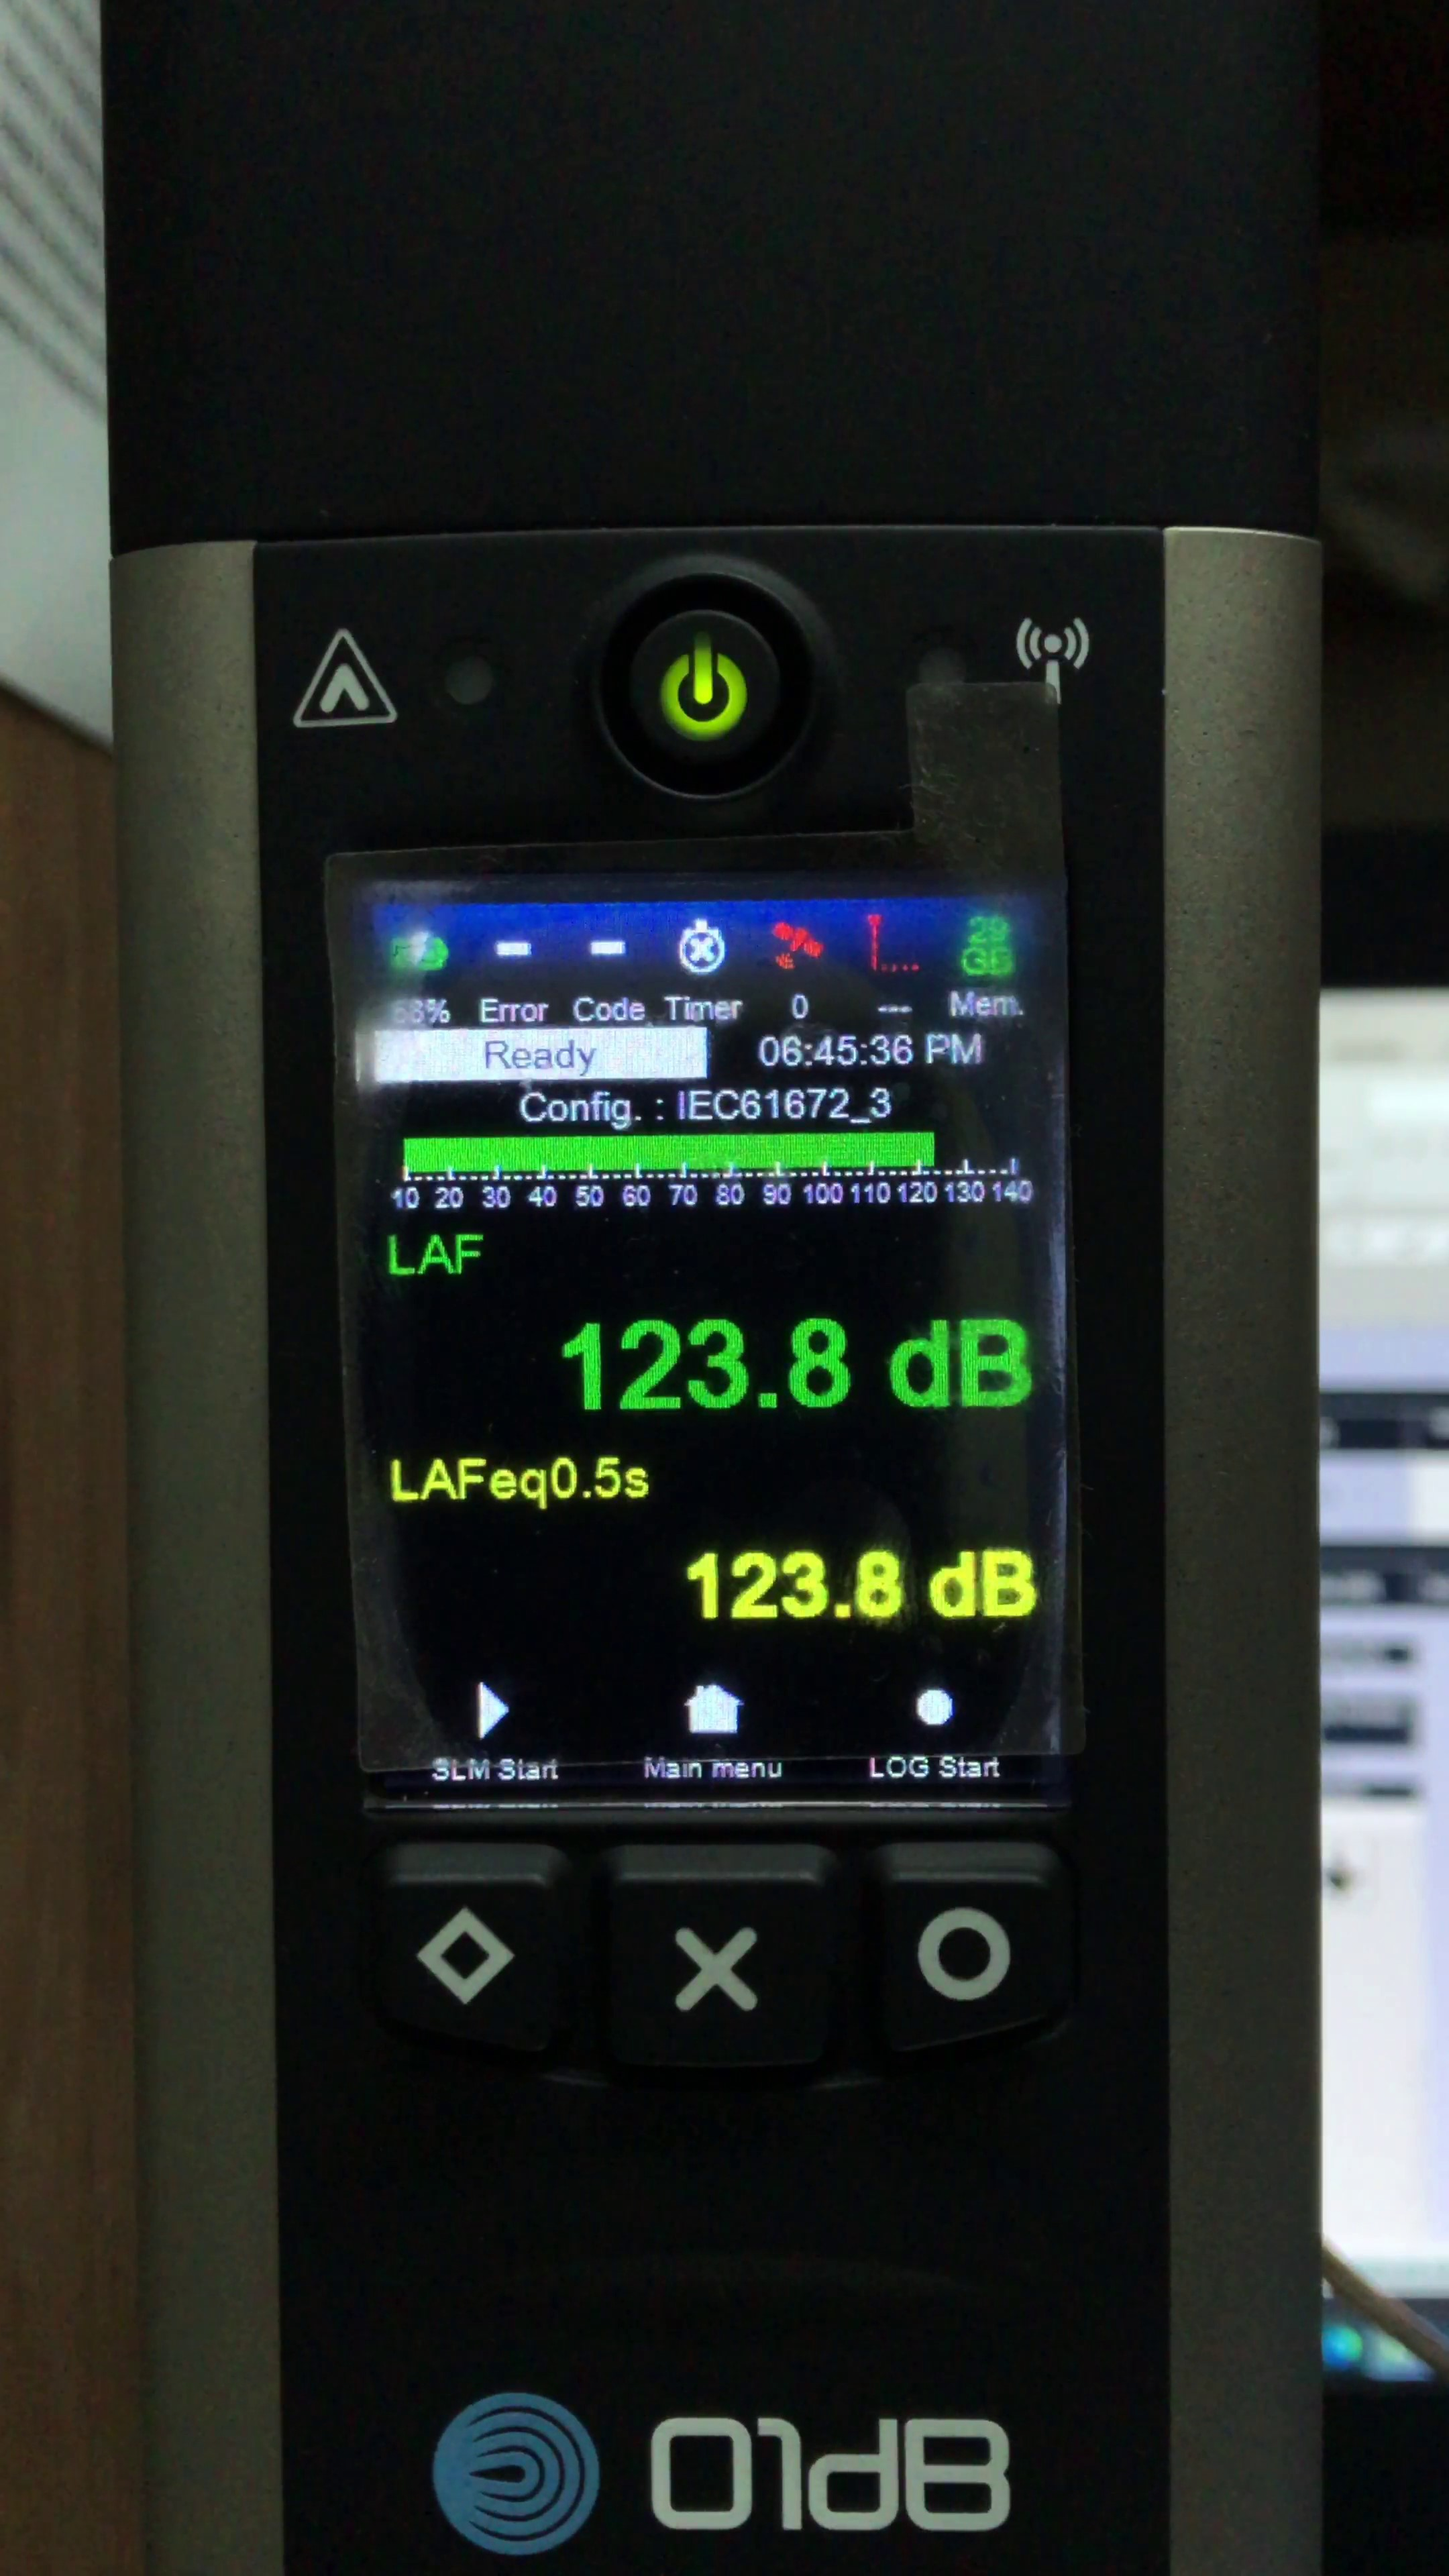
\includegraphics[height=7.2cm]{3_reconocimiento/Figs/slm_screen}
\end{figure}

Para el filtro gaussiano se empleó $\sigma_x = \sigma_y = \num{1.5}$.
Luego, con el fin de simplificar el cálculo del descriptor SIFT, se escala la imagen de un dígito y se rellenan los píxeles faltantes para conformar una imagen de $32 \times 32$.
Después, se eligen cuatro puntos clave que corresponden a los centros de cada cuadrante como se presenta en la siguiente figura.
%
\begin{figure}[h]
    \caption{Puntos clave para el cálculo del descriptor SIFT de una imagen de un dígito.}
    \label{fig:keypoints_SIFT}
    \centering
    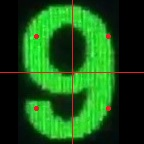
\includegraphics[height=5cm]{3_Reconocimiento/Figs/keypoints_SIFT}
\end{figure}

En esos puntos se calcula el descriptor SIFT, no sin previamente haber umbralizado la imagen redimensionada con el método de Otsu.
De forma tal que queda un vector de características con $512$ valores para cada muestra.

Una breve implementación de este procesamiento se presenta en el código~\ref{code:test_samples_code}, que posteriormente será usado en la aplicación desarrollada para automatizar la calibración de sonómetros.

En la siguiente figura se muestran los resultados de los pasos 1 al 3 del algoritmo~\ref{alg:image_recongnition} para una muestra de entrenamiento del número $5$.
%
\tikzmath{\x1 = 6.3;}
\begin{figure}[hb!]
    \caption{Resultados de procesamiento de una muestra de entrenamiento del número $5$.}
    \label{fig:train_sample5_processing}
    \centering
    \begin{subfigure}[t]{0.48\textwidth}
        \centering
        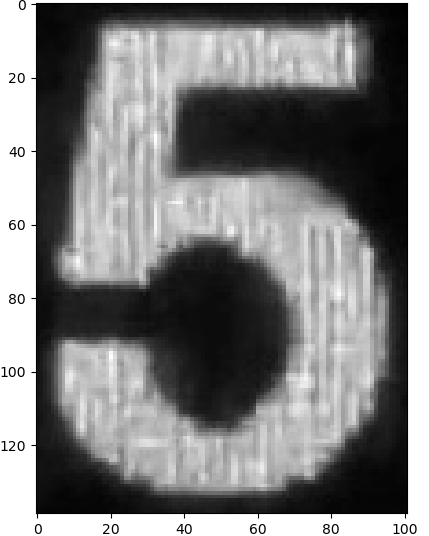
\includegraphics[height=\x1cm]{3_Reconocimiento/Figs/train_sample5_original}
        \caption{Imagen original en escala de grises.}
    \end{subfigure}
    \hfill
    \begin{subfigure}[t]{0.48\textwidth}
        \centering
        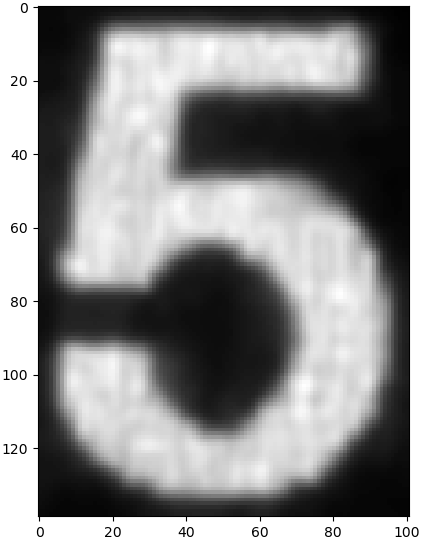
\includegraphics[height=\x1cm]{3_Reconocimiento/Figs/train_sample5_filtered}
        \caption{Imagen filtrada con filtro gausiano \hyperref[sec:gaussian_filter]{(paso 1)}.}
    \end{subfigure}
    \\[+1em]
    \begin{subfigure}[t]{0.48\textwidth}
        \centering
        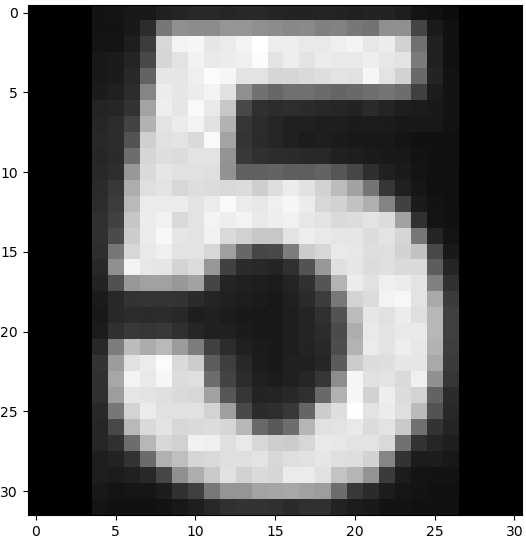
\includegraphics[height=\x1cm]{3_Reconocimiento/Figs/train_sample5_padded}
        \caption{Imagen escalada y con \emph{padding} \hyperref[sec:padding]{(paso 2)}.}
    \end{subfigure}
    \hfill
    \begin{subfigure}[t]{0.48\textwidth}
        \centering
        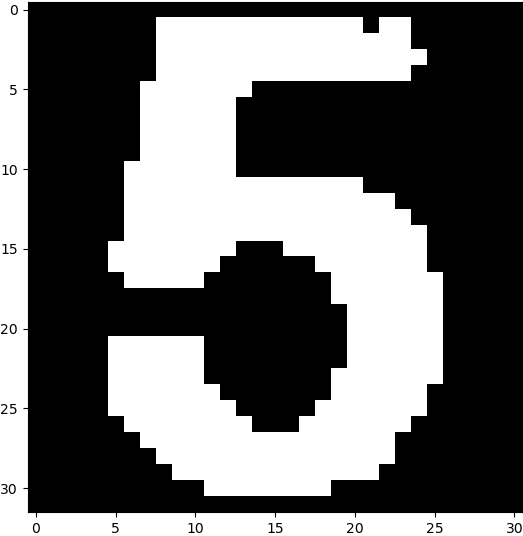
\includegraphics[height=\x1cm]{3_Reconocimiento/Figs/train_sample5_otsu}
        \caption{Imagen binarizada con el método de Otsu \hyperref[sec:segmentation]{(paso 3)}}
    \end{subfigure}
\end{figure}

Para el \hyperref[sec:sift_descriptor]{paso 4}, con las últimas líneas del código~\ref{code:test_samples_code} también se grafican los vectores de características.
En la figura~\ref{fig:train_samples_features} se muestran los resultados de una muestra de cada clase $2$, $5$ y $7$.
%
\begin{figure}[h]
    \caption{Vectores de características de una muestra de cada clase $2$, $5$ y $7$.}
    \label{fig:train_samples_features}
    \centering
    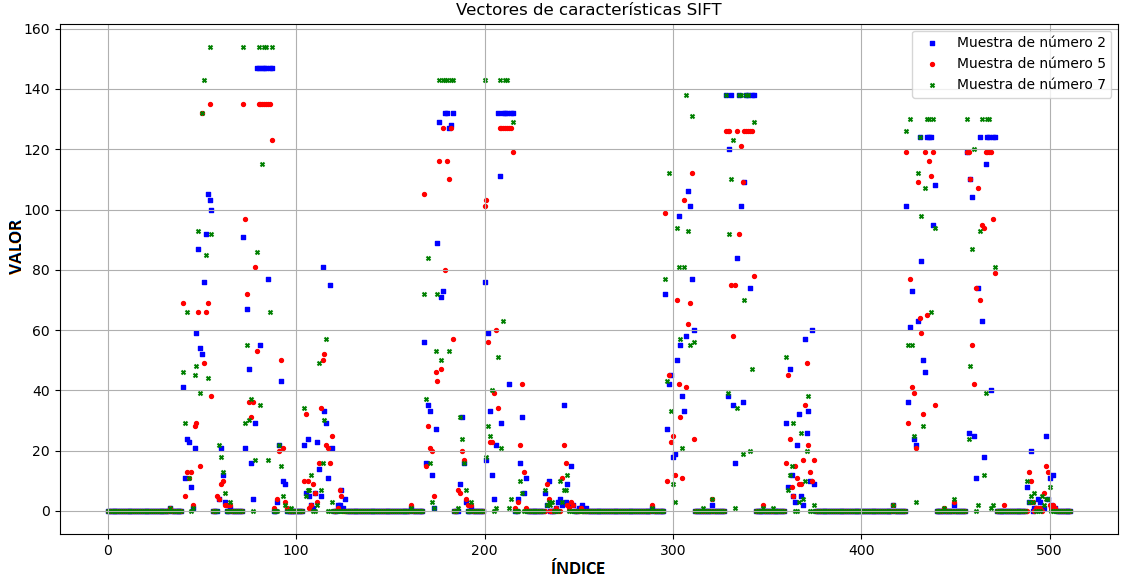
\includegraphics[width=0.8\textwidth]{3_Reconocimiento/Figs/train_samples_features}
\end{figure}

Ahora, el código~\ref{code:test_samples_code} se puede ejecutar iterativamente para leer todas las imágenes de un conjunto de entrenamiento con aproximadamente entre $40$ y $100$ muestras por cada clase.
Luego, para los pasos \hyperref[sec:kpca_reduction]{5} y \hyperref[sec:nb_classifier]{6}, complementando con el código~\ref{code:features_extracting}, se efectúa la extracción de características y se entrena el clasificador bayesiano normal.
La reducción de dimensionalidad se hizo hasta un valor de $d = 16$, empíricamente seleccionado según los resultados de clasificación obtenidos.

Finalmente, para una muestra dada de prueba, se efectúa el mismo procesamiento de la imagen con el código~\ref{code:test_samples_code}, y la extracción y clasificación se efectúa con el código~\ref{code:sample_classifying}.

Durante los primeros ensayos del algoritmo se pudo notar que si las condiciones de captura de la imagen no son controladas, factores como el desenfoque de la cámara, la alta exposición controlada por el diafragma de la cámara, reflejos, destellos de luz o bajo contraste, pueden afectar significativamente la clasificación.
Por ejemplo, en la figura~\ref{fig:good_bad_conditions} se presenta una comparación entre tres números fotografiados en condiciones controladas y no controladas, y el respectivo resultado de procesamiento.

\tikzmath{\x1 = 5.3;}
\begin{figure}[hp!]
    \caption{Comparación del procesamiento de imágenes tomadas en condiciones controladas y no controladas.}
    \label{fig:good_bad_conditions}
    \centering
    \begin{subfigure}[t]{0.3\textwidth}
        \centering
        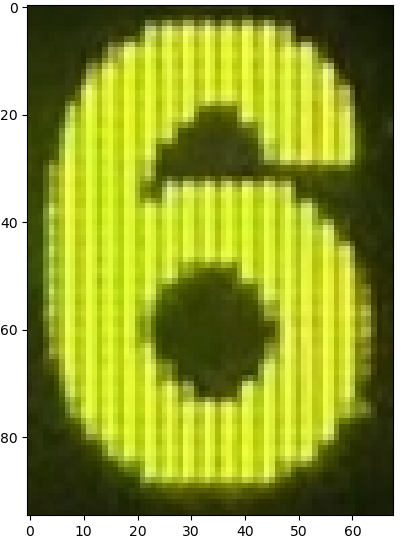
\includegraphics[height=\x1cm]{3_Reconocimiento/Figs/test_sample6_good_original}
        \caption{Imagen original en condiciones controladas.}
        \label{fig:good_conditions_original}
    \end{subfigure}
    \hfill
    \begin{subfigure}[t]{0.3\textwidth}
        \centering
        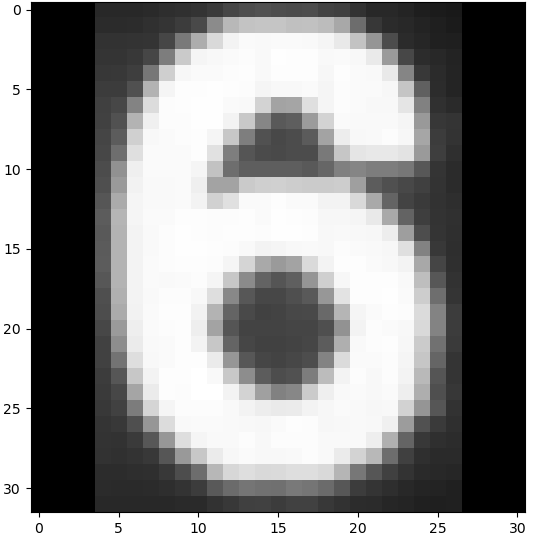
\includegraphics[height=\x1cm]{3_Reconocimiento/Figs/test_sample6_good_padded}
        \caption{Imagen hasta el paso 2 en condiciones controladas.}
        \label{fig:good_conditions_padded}
    \end{subfigure}
    \hfill
    \begin{subfigure}[t]{0.3\textwidth}
        \centering
        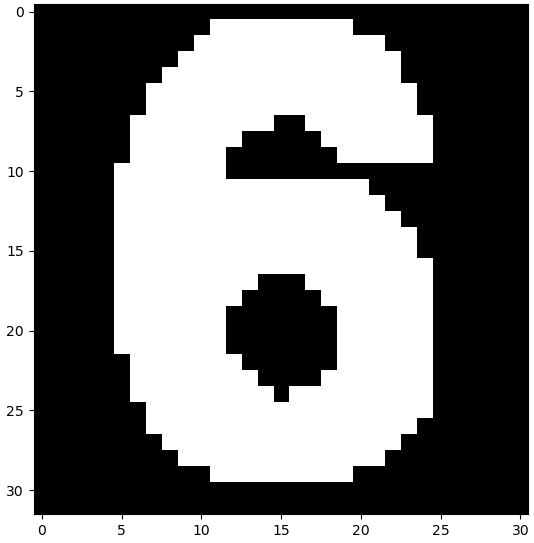
\includegraphics[height=\x1cm]{3_Reconocimiento/Figs/test_sample6_good_otsu}
        \caption{Imagen hasta el paso 3 en condiciones controladas.}
    \end{subfigure}
    \\[+1em]
    \begin{subfigure}[t]{0.3\textwidth}
        \centering
        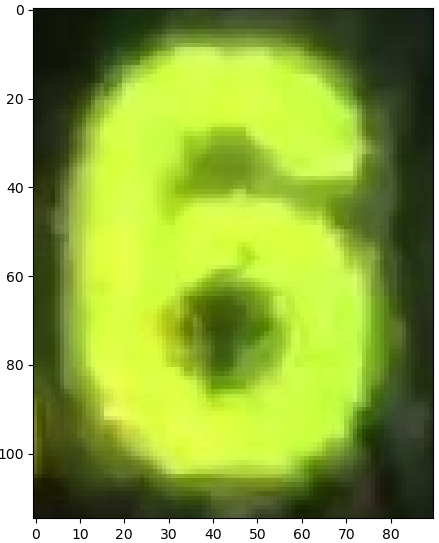
\includegraphics[height=\x1cm]{3_Reconocimiento/Figs/test_sample6_bad_original1}
        \caption{Imagen original en condiciones no controladas.}
    \end{subfigure}
    \hfill
    \begin{subfigure}[t]{0.3\textwidth}
        \centering
        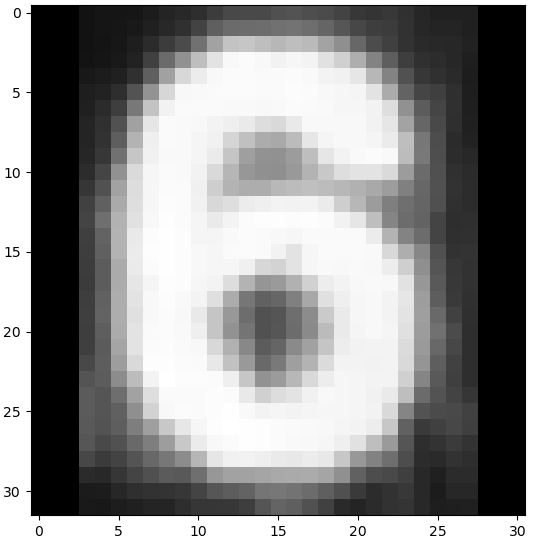
\includegraphics[height=\x1cm]{3_Reconocimiento/Figs/test_sample6_bad_padded1}
        \caption{Imagen hasta el paso 2 en condiciones no controladas.}
    \end{subfigure}
    \hfill
    \begin{subfigure}[t]{0.3\textwidth}
        \centering
        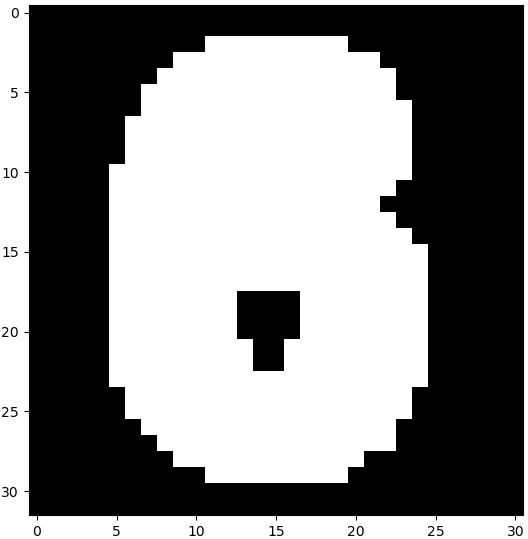
\includegraphics[height=\x1cm]{3_Reconocimiento/Figs/test_sample6_bad_otsu1}
        \caption{Imagen hasta el paso 3 en condiciones no controladas.}
    \end{subfigure}
    \\[+1em]
    \begin{subfigure}[t]{0.3\textwidth}
        \centering
        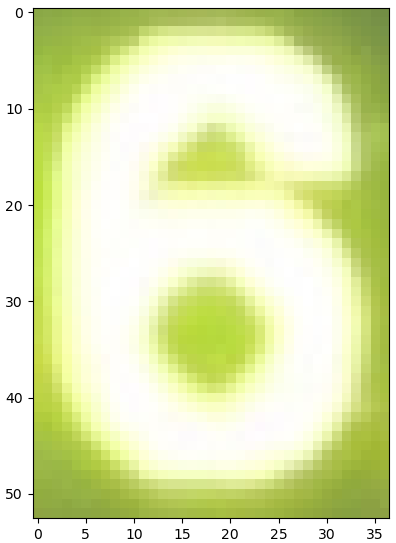
\includegraphics[height=\x1cm]{3_Reconocimiento/Figs/test_sample6_bad_original2}
        \caption{Imagen original en condiciones no controladas.}
    \end{subfigure}
    \hfill
    \begin{subfigure}[t]{0.3\textwidth}
        \centering
        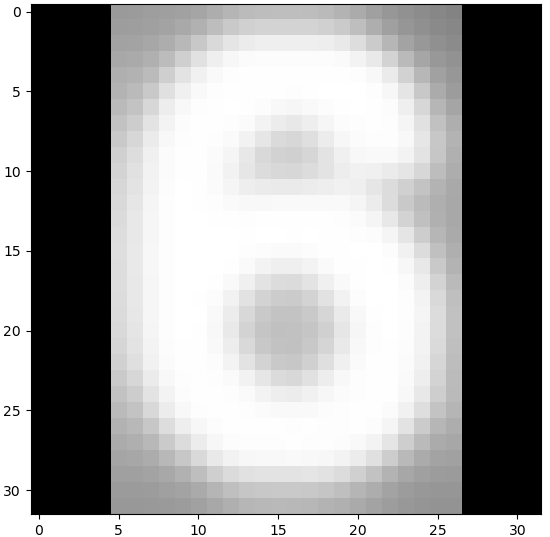
\includegraphics[height=\x1cm]{3_Reconocimiento/Figs/test_sample6_bad_padded2}
        \caption{Imagen hasta el paso 2 en condiciones no controladas.}
    \end{subfigure}
    \hfill
    \begin{subfigure}[t]{0.3\textwidth}
        \centering
        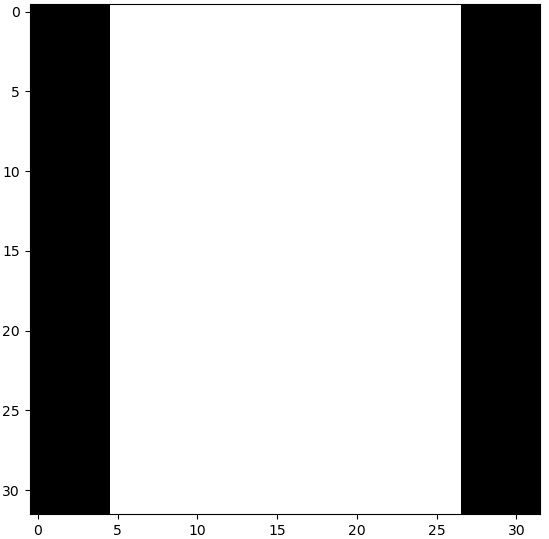
\includegraphics[height=\x1cm]{3_Reconocimiento/Figs/test_sample6_bad_otsu2}
        \caption{Imagen hasta el paso 3 en \\ condiciones no controladas.}
    \end{subfigure}
\end{figure}

La precisión del clasificador se puede medir fácilmente con una matriz de confusión, en la que directamente se identifican los falsos y verdaderos positivos.
La matriz de confusión se genera rápidamente con el código~\ref{code:confusion_matrix}.
Se armaron dos conjuntos de prueba, uno en condiciones no controladas y otro en que sí, y se probó el clasificador en ambos.
En la figura~\ref{fig:confusion_matrix_bad} se muestra la matriz de confusión para el primer conjunto (condiciones no controladas) y en la figura~\ref{fig:confusion_matrix_good} la del segundo (condiciones controladas).
\vfill
%
\begin{figure}[h!]
    \caption{Matriz de confusión del clasificador bayesiano propuesto para el conjunto de imágenes tomadas en condiciones no controladas.}
    \label{fig:confusion_matrix_bad}
    \centering
    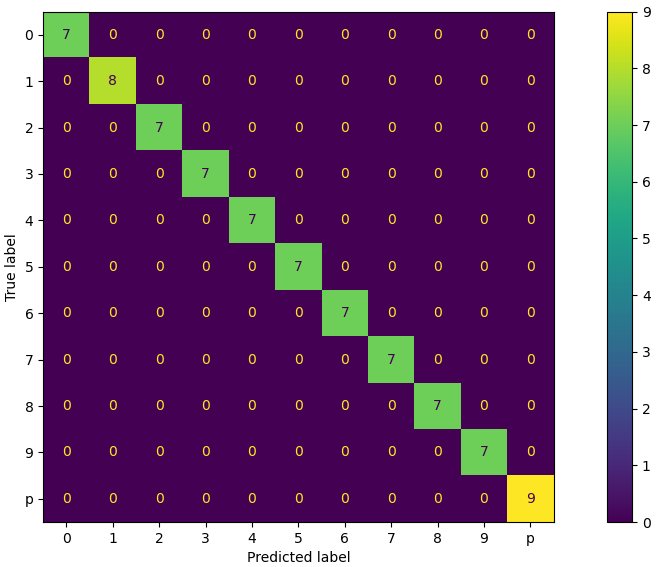
\includegraphics[width=0.5\textwidth]{3_Reconocimiento/Figs/confusion_matrix_good}
\end{figure}
%
\begin{figure}[h!]
    \caption{Matriz de confusión del clasificador bayesiano propuesto para el conjunto de imágenes tomadas en condiciones controladas.}
    \label{fig:confusion_matrix_good}
    \centering
    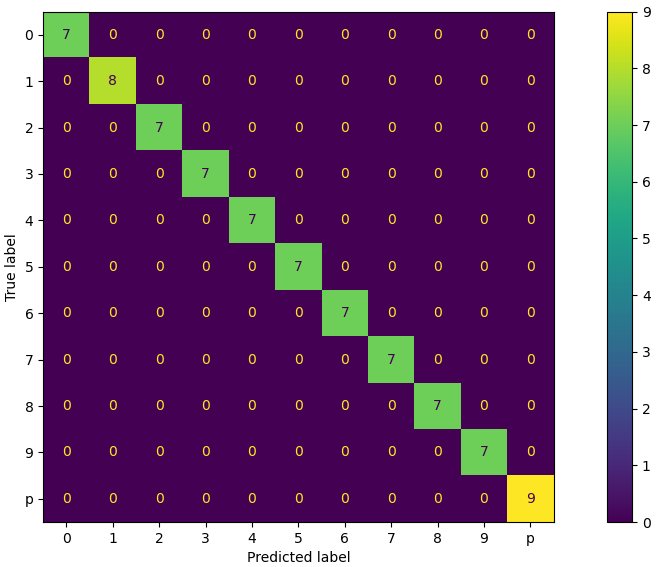
\includegraphics[width=0.5\textwidth]{3_Reconocimiento/Figs/confusion_matrix_good}
\end{figure}


\section*{Discusión}

Los resultados obtenidos demuestran un funcionamiento satisfactorio en general, tanto del procesamiento de las imágenes como del clasificador.
Aunque evidentemente es un método simplificado, resulta ser eficaz y eficiente, pues cumple con el objetivo de reconocimiento de caracteres empleando pocos recursos computacionales y cortos tiempos de entrenamiento del clasificador y del procesamiento de las imágenes, lo que permite que el método sea empleado en ordenadores con baja capacidad de procesamiento y en aplicaciones de funcionamiento en tiempo real, como se pretende en este proyecto.
Aunque el clasificador bayesiano es de las técnicas más sencillas de aprendizaje de máquina, tiene un desempeño aceptable en muchas aplicaciones reales y no requiere una base de datos de entrenamiento demasiado extensa \citepalias{Scikit-learndevelopers2022}.

Particularmente, cada una de las etapas de procesamiento resulta ser crucial en el resultado.
Por ejemplo la etapa de suavizado permite eliminar variaciones de intensidad de alta frecuencia como las irregularidades en el relleno de los dígitos debidas a la construcción de la pantalla del sonómetro, como en pantallas led, por ejemplo (cf.~\ref{fig:good_conditions_original} y~\ref{fig:good_conditions_padded}).
Sin este suavizado es posible que en la umbralización no se obtengan segmentos homogéneos que representen correctamente un dígito.
La binarización de la imagen, buscando el umbral con el método de Otsu, garantiza que se haga una discriminación correcta entre el fondo de la pantalla y el dígito, en función de la distribución de las intensidades de píxeles, esto aporta confiabilidad en la segmentación independientemente de la forma y color de los números.
Y el descriptor SIFT es bien conocido por su robustez frente a transformaciones afines o cambios en el punto de vista 3D, lo que contribuye a asegurar la eficacia en la medición de características aun cuando hay variaciones en la posición de la cámara respecto a la pantalla del sonómetro;
además, que esté basado en la dirección de los gradientes, lo hace adecuado para cuantizar de algún modo las formas de los contornos de los dígitos.

No obstante, a pesar de la eficiencia y simplicidad del clasificador bayesiano normal, lo cierto es que el resultado de clasificación es bastante sensible si se obtienen resultados erróneos en el procesamiento anterior.
Por ejemplo, por efectos de bajo contraste o desenfoques que deforman los segmentos, podría haber confusiones en la clasificación, principalmente en clases que son muy similares en sus características, como entre el $6$ y el $8$ o entre el $9$ y el $8$, pues al deformarse el segmento a causa de esos ruidos, el $6$ o el $9$ cierran el trazo faltante y se asemejan a un $8$, o alguno de los huecos se rellena y se asemejan a un $0$.
Sin embargo, en los ensayos del sistema de reconocimiento se pudo comprobar que esto ocurre cuando la posición o configuración de la cámara no es la adecuada y los efectos del desenfoque o la iluminación son más pronunciados.
Cuando las condiciones de captura de la imagen son controladas (por ejemplo, ajustando en la cámara la distancia focal y la apertura del diafragma adecuadas, limpiando la pantalla del equipo para evitar borrosidad e incluso buscando una posición apropiada del sonómetro y la cámara para mitigar las reflexiones de las fuentes de luz del lugar), la eficacia del clasificador es de un $100\%$, como se puede notar en la matriz de confusión de la figura~\ref{fig:confusion_matrix_good}.

%  ╦┌┬┐┌─┐┬  ┌─┐┌┬┐┌─┐┌┐┌┌┬┐┌─┐┌─┐┬┌─┐┌┐┌
%  ║│││├─┘│  ├┤ │││├┤ │││ │ ├─┤│  ││ ││││
%  ╩┴ ┴┴  ┴─┘└─┘┴ ┴└─┘┘└┘ ┴ ┴ ┴└─┘┴└─┘┘└┘

\chapter{Implementación de los procedimientos de calibración}

En este capítulo se describe el desarrollo y arquitectura de software de las aplicaciones diseñadas para la calibración periódica de calibradores acústicos de acuerdo con la \mbox{IEC 60942}~\citeyearpar{IEC_TC29_2017} (tomando como base un modelamiento en GRAFCET) y de sonómetros de acuerdo con la norma \mbox{IEC 61672--3}~\citeyearpar{IEC_TC29_2013_1} (usando el sistema de reconocimiento de caracteres del capítulo~\ref{ch:image_recognition}).
El desarrollo del \emph{software} está publicado en el siguiente repositorio de GitHub:

    {\footnotesize\url{https://github.com/jfBranch/unal-acoustic-metrology.git}}


\section{Automatización de la calibración periódica de calibradores acústicos}
\label{sec:acoustic_calibrators_automation}
Siguiendo el método normalizado descrito en la sección~\ref{subsec:acoustic_calibrators_calibration_description} y el algoritmo de la figura~\ref{fig:acoustic_calibrator_calibration_flowchart}, se modeló la secuencia de calibración en un gráfico de etapas y transiciones explicado en la siguiente sección.

\subsection{GRAFCET descriptivo del proceso}
Para dar mayor claridad, en la figura~\ref{fig:GRAFCET_principal} se presenta la secuencia principal en la que se hacen llamadas a subrutinas mediante las etapas macro.
Los GRAFCET de las subrutinas se muestran en las figuras~\ref{fig:GRAFCET_micsens} a la~\ref{fig:GRAFCET_noise_dut}.
\vfill
\clearpage

\begin{figure}[!hp]
    \caption{GRAFCET de la rutina principal de la calibración periódica de calibradores acústicos.}
    \label{fig:GRAFCET_principal}
    \centering
    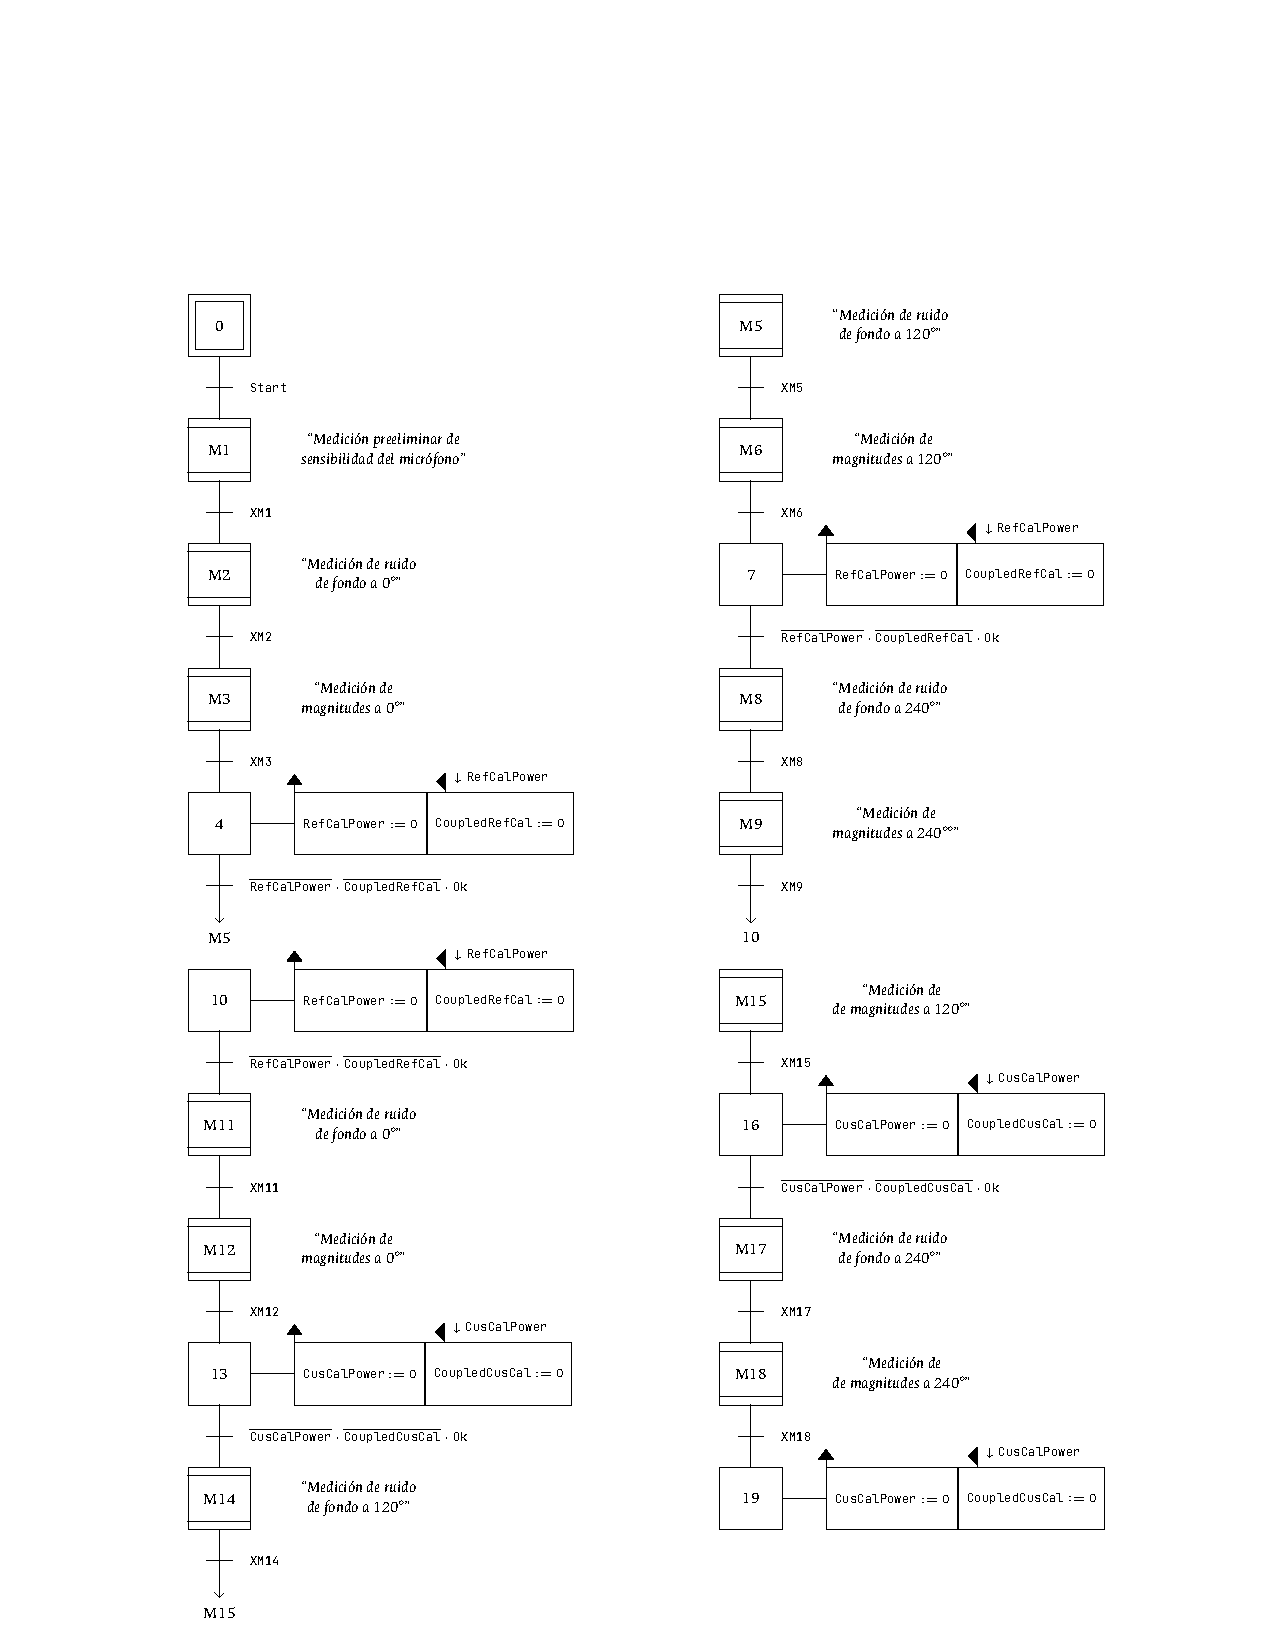
\includegraphics[height=0.92\textheight]{4_Implementación/principalGRAFCET}
    \caption*{\footnotesize Fuente: Elaboración propia.}
\end{figure}
%
\begin{sidewaysfigure}[!hp]
    \caption{GRAFCET's de las subrutinas para la calibración periódica de calibradores acústicos.}
    \label{fig:GRAFCET_subrutines}
    \begin{subfigure}[t]{0.48\textwidth}
        \caption{Subrutina para la etapa macro $1$: Medición preeliminar de sensibilidad del micrófono.}
        \label{fig:GRAFCET_micsens}
        \centering
        \begin{tikzpicture}[font=\scriptsize]
            \begin{Encap}{0,0}{M1}{Mic Sensibility Measurement}
                \Etape[0,0]{E1}
                \ActionX{XE1}{\tiny $\texttt{CoupledRefCal} \defeq 1$}
                \ActionActiv{XE1}
                \Action{XE1}{\tiny \texttt{RefCalPower} $\defeq 1$}
                \ActionEvenement{XE1}{\tiny $\uparrow\texttt{CoupledRefCal}$}
                \TransitionRecept[VXE1]{E1}{\tiny $\texttt{RefCalPower} \cdot \texttt{CoupledRefCal} \cdot \texttt{Ok}$}
                \node(TE1') [below=0cm of VXE1]{}; \node(VTE1')[below=2em of TE1']{}; \draw (TE1') -- (VTE1');
                \DecaleNoeudx[11]{TE1'}{TE1r}
                \DecaleNoeudx[11]{VTE1}{VTE1r}
                \ConvOU{TE1'}{TE1r}{L20}
                \Etape[L20]{20}
                \ActionX{X20}{\tiny \texttt{MeasMicSens}}
                \ActionCond{X20}{\tiny $\qty{10}{\s}$/\texttt{X20}}
                \Action{X20}{\tiny \texttt{MeasFinished}}
                \ActionCond{X20}{\tiny $\qty{5}{\s}$/\texttt{MeasMicSens}}
                \DivOU{X20}{-4/L20a, 5/L20b}
                \Transition[L20a]{20a}
                \node[right=0.1 of L20a, align=left]{\tiny $\texttt{MeasFinished} \cdot$ \\ \tiny $[\qty{380}{\mV} \le \mathit{Sens} \le \qty{460}{\mV}]$};
                \Transition[L20b]{20b}
                \node [right=0.1 of L20b, align=left]
                {\tiny $\texttt{MeasFinished} \cdot$ \\ \tiny $([\qty{380}{\mV} \ge \mathit{Sens}] +$ \\ \tiny $[\mathit{Sens} \ge \qty{480}{\mV}])$};
                \Etape[VT20b]{21}
                \ActionX{X21}{\tiny \texttt{RepeatDialog}}
                \DivOU{X21}{-3/L21a,3/L21b}
                \TransitionRecept[L21a]{21a}{\tiny $\texttt{X21} \cdot \overline{\texttt{Ok}}$}
                \TransitionRecept[L21b]{21b}{\tiny $\texttt{X21} \cdot \texttt{Ok}$}
                \node (paso) [right=1em of TE1r]{};
                \Lien{T21b}{paso}{VTE1r}
                \Etape[VT21a]{22}
                \node[right=0.2 of X22, align=center]{\textit{``Suspende la} \\ \textit{secuencia principal''}};
                \DecaleNoeudy[8.8]{L20a}{nS1}
                \Etape[nS1]{S1}
                \draw (L20a) -- (XS1);
            \end{Encap}
        \end{tikzpicture}
        \caption*{\footnotesize Fuente: Elaboración propia.}
    \end{subfigure}
    \hfill
    \begin{subfigure}[t]{0.48\textwidth}
        \caption{Subrutina para la etapa macro $2$: Medición de ruido de fondo a $\qty{5}{\degree}$ con el calibrador patrón.}
        \label{fig:GRAFCET_standard_noise0}
        \centering
        \begin{tikzpicture}[font=\scriptsize]
            \begin{Encap}{0,0}{M2}{Background Noise Standard Calibrator}
                \Etape[0,0]{E2}
                \ActionX{XE2}{\tiny $\texttt{RefCalOrient} \defeq 0$}
                \ActionActiv{XE2}
                \Action{XE2}{\tiny \texttt{RefCalPower} $\defeq 0$}
                \ActionEvenement{XE2}{\tiny $\uparrow\texttt{RotatedRefCal}$}
                \TransitionRecept[VXE2]{E2}{\tiny $\overline{\texttt{RefCalPower}} \cdot \texttt{CoupledRefCal} \cdot \texttt{Ok}$}
                \node(TE2') [below=0cm of VXE2]{}; \node(VTE2')[below=2em of TE2']{}; \draw (TE2') -- (VTE2');
                \DecaleNoeudx[11]{TE2'}{TE2r}
                \DecaleNoeudx[11]{VTE2}{VTE2r}
                \ConvOU{TE2'}{TE2r}{L23}
                \Etape[L23]{23}
                \ActionX{X23}{\tiny \texttt{MeasBackNoise}}
                \ActionCond{X23}{\tiny $\qty{3}{\s}$/\texttt{X23}}
                \Action{X23}{\tiny \texttt{MeasFinished}}
                \ActionCond{X23}{\tiny $\qty{7}{\s}$/\texttt{MeasBackNoise}}
                \DivOU{X23}{-4/L23a, 4.5/L23b}
                \Transition[L23a]{23a}
                \node[right=0.1 of L23a, align=left]
                {\tiny $\texttt{MeasFinished} \cdot$ \\ \tiny $[\mathit{Noise} \le L_{\mathrm{spec}} - \qty{30}{\dB}]$};
                \Transition[L23b]{23b}
                \node [right=0.1 of L23b, align=left]
                {\tiny $\texttt{MeasFinished} \cdot$ \\ \tiny $[\mathit{Noise} \ge L_{\mathrm{spec}} - \qty{30}{\dB}]$};
                \Etape[VT23b]{24}
                \ActionX{X24}{\tiny \texttt{RepeatDialog}}
                \DivOU{X24}{-3/L24a,3/L24b}
                \TransitionRecept[L24a]{24a}{\tiny $\texttt{X24} \cdot \overline{\texttt{Ok}}$}
                \TransitionRecept[L24b]{24b}{\tiny $\texttt{X24} \cdot \texttt{Ok}$}
                \node (paso) [right=2em of TE2r]{};
                \Lien{T24b}{paso}{VTE2r}
                \Etape[VT24a]{25}
                \node[right=0.2 of X25, align=center]{\textit{``Suspende la} \\ \textit{secuencia principal''}};
                \DecaleNoeudy[8.8]{L23a}{nS2}
                \Etape[nS2]{S2}
                \draw (L23a) -- (XS2);
            \end{Encap}
        \end{tikzpicture}
        \caption*{\footnotesize Fuente: Elaboración propia.}
    \end{subfigure}
\end{sidewaysfigure}
%
\begin{sidewaysfigure}[!hp]
    \ContinuedFloat
    \caption{GRAFCET's de las subrutinas para la calibración periódica de calibradores acústicos (continuación).}
    \begin{subfigure}[t]{0.33\textwidth}
        \caption{Subrutina para las etapas macro $\numlist{3;6;9}$: Medición de magnitudes con el calibrador patrón.}
        \label{fig:GRAFCET_standard_quantities}
        \centering
        \begin{tikzpicture}[font=\scriptsize]
            \begin{Encap}{0,0}{M3 (M6 o M9)}{Quantities Measurement Standard Cal}
                \EtapeTransition[0,0]{E3}{\tiny $\texttt{RefCalPower} \defeq 1$}{\tiny $\texttt{RefCalPower} \cdot \texttt{Ok}$}
                \ActionActiv{XE3}
                \LienTE[3]{TE3}
                \EtapeTransition[VTE3]{26}{\tiny \texttt{MeasQuantities}}{\tiny \texttt{MeasFinished}}
                \ActionCond{X26}{\tiny $\qty{18}{\s}$/\texttt{X26}}
                \Action{X26}{\tiny \texttt{MeasFinished}}
                \ActionCond{X26}{\tiny $\qty{30}{\s}$/\texttt{MeasQuantities}}
                \Etape{S3}
            \end{Encap}
        \end{tikzpicture}
        \caption*{\footnotesize Fuente: Elaboración propia.}
    \end{subfigure}
    \hfill
    \begin{subfigure}[t]{0.55\textwidth}
        \caption{Subrutina para las etapas macro $\numlist{5; 8}$: Medición de ruido de fondo a $\qty{120}{\degree}$ y $\qty{240}{\degree}$ con el calibrador patrón.}
        \label{fig:GRAFCET_noise_standard}
        \centering
        \begin{tikzpicture}[font=\scriptsize]
            \begin{Encap}{0,0}{M5 (M8)}{Background Noise Standard Calibrator}
                \Etape[0,0]{E5}
                \ActionX{XE5}{\tiny $\texttt{RefCalOrient} \defeq \texttt{RefCalOrient} + 120$}
                \ActionActiv{XE5}
                \Action{XE5}{\tiny \texttt{CoupledRefCal} $\defeq 1$}
                \ActionEvenement{XE5}{\tiny $\uparrow\texttt{RotatedRefCal}$}
                \TransitionRecept[VXE5]{E5}{\tiny $\overline{\texttt{RefCalPower}} \cdot \texttt{CoupledRefCal} \cdot \texttt{Ok}$}
                \node(TE5') [below=0cm of VXE5]{}; \node(VTE5')[below=2em of TE5']{}; \draw (TE5') -- (VTE5');
                \DecaleNoeudx[11]{TE5'}{TE5r}
                \DecaleNoeudx[11]{VTE5}{VTE5r}
                \ConvOU{TE5'}{TE5r}{L27}
                \Etape[L27]{27}
                \ActionX{X27}{\tiny \texttt{MeasBackNoise}}
                \ActionCond{X27}{\tiny $\qty{3}{\s}$/\texttt{X27}}
                \Action{X27}{\tiny \texttt{MeasFinished}}
                \ActionCond{X27}{\tiny $\qty{7}{\s}$/\texttt{MeasBackNoise}}
                \DivOU{X27}{-4/L27a, 4.5/L27b}
                \Transition[L27a]{27a}
                \node[right=0.1 of L27a, align=left]
                {\tiny $\texttt{MeasFinished} \cdot$ \\ \tiny $[\mathit{Noise} \le L_{\mathrm{spec}} - \qty{30}{\dB}]$};
                \Transition[L27b]{27b}
                \node [right=0.1 of L27b, align=left]
                {\tiny $\texttt{MeasFinished} \cdot$ \\ \tiny $[\mathit{Noise} \ge L_{\mathrm{spec}} - \qty{30}{\dB}]$};
                \Etape[VT27b]{28}
                \ActionX{X28}{\tiny \texttt{RepeatDialog}}
                \DivOU{X28}{-3/L28a,3/L28b}
                \TransitionRecept[L28a]{28a}{\tiny $\texttt{X28} \cdot \overline{\texttt{Ok}}$}
                \TransitionRecept[L28b]{28b}{\tiny $\texttt{X28} \cdot \texttt{Ok}$}
                \node (paso) [right=2em of TE5r]{};
                \Lien{T28b}{paso}{VTE5r}
                \Etape[VT28a]{29}
                \node[right=0.2 of X29, align=center]{\textit{``Suspende la} \\ \textit{secuencia principal''}};
                \DecaleNoeudy[8.8]{L27a}{nS5}
                \Etape[nS5]{S5}
                \draw (L27a) -- (XS5);
            \end{Encap}
        \end{tikzpicture}
        \caption*{\footnotesize Fuente: Elaboración propia.}
    \end{subfigure}
\end{sidewaysfigure}
%
\begin{sidewaysfigure}[!hp]
    \ContinuedFloat
    \caption{GRAFCET's de las subrutinas para la calibración periódica de calibradores acústicos (continuación).}
    \begin{subfigure}[t]{0.48\textwidth}
        \caption{Subrutina para la etapa macro $11$: Medición de ruido de fondo a $\qty{0}{\degree}$ con el calibrador bajo prueba.}
        \label{fig:GRAFCET_noise0_dut}
        \centering
        \begin{tikzpicture}[font=\scriptsize]
            \begin{Encap}{0,0}{M11}{Background Noise Customer Calibrator}
                \Etape[0,0]{E11}
                \ActionX{XE11}{\tiny $\texttt{CusCalOrient} \defeq 0$}
                \ActionActiv{XE11}
                \Action{XE11}{\tiny \texttt{CusCalPower} $\defeq 0$}
                \ActionEvenement{XE11}{\tiny $\uparrow\texttt{RotatedRefCal}$}
                \TransitionRecept[VXE11]{E11}{\tiny $\overline{\texttt{CusCalPower}} \cdot \texttt{CoupledCusCal} \cdot \texttt{Ok}$}
                \node(TE11') [below=0cm of VXE11]{}; \node(VTE11')[below=2em of TE11']{}; \draw (TE11') -- (VTE11');
                \DecaleNoeudx[11]{TE11'}{TE11r}
                \DecaleNoeudx[11]{VTE11}{VTE11r}
                \ConvOU{TE11'}{TE11r}{L30}
                \Etape[L30]{30}
                \ActionX{X30}{\tiny \texttt{MeasBackNoise}}
                \ActionCond{X30}{\tiny $\qty{3}{\s}$/\texttt{X30}}
                \Action{X30}{\tiny \texttt{MeasFinished}}
                \ActionCond{X30}{\tiny $\qty{7}{\s}$/\texttt{MeasBackNoise}}
                \DivOU{X30}{-4/L30a, 4.5/L30b}
                \Transition[L30a]{23a}
                \node[right=0.1 of L30a, align=left]
                {\tiny $\texttt{MeasFinished} \cdot$ \\ \tiny $[\mathit{Noise} \le L_{\mathrm{spec}} - \qty{30}{\dB}]$};
                \Transition[L30b]{30b}
                \node [right=0.1 of L30b, align=left]
                {\tiny $\texttt{MeasFinished} \cdot$ \\ \tiny $[\mathit{Noise} \ge L_{\mathrm{spec}} - \qty{30}{\dB}]$};
                \Etape[VT30b]{31}
                \ActionX{X31}{\tiny \texttt{RepeatDialog}}
                \DivOU{X31}{-3/L31a,3/L31b}
                \TransitionRecept[L31a]{31a}{\tiny $\texttt{X31} \cdot \overline{\texttt{Ok}}$}
                \TransitionRecept[L31b]{31b}{\tiny $\texttt{X31} \cdot \texttt{Ok}$}
                \node (paso) [right=2em of TE11r]{};
                \Lien{T31b}{paso}{VTE11r}
                \Etape[VT31a]{32}
                \node[right=0.2 of X32, align=center]{\textit{``Suspende la} \\ \textit{secuencia principal''}};
                \DecaleNoeudy[8.8]{L30a}{nS11}
                \Etape[nS11]{S11}
                \draw (L30a) -- (XS11);
            \end{Encap}
        \end{tikzpicture}
        \caption*{\footnotesize Fuente: Elaboración propia.}
    \end{subfigure}
    \hfill
    \begin{subfigure}[t]{0.48\textwidth}
        \caption{Subrutina para las etapas macro $\numlist{14;17}$: Medición de ruido de fondo a $\qty{120}{\degree}$ y $\qty{240}{\degree}$ con el calibrador bajo prueba.}
        \label{fig:GRAFCET_noise_dut}
        \centering
        \begin{tikzpicture}[font=\scriptsize]
            \begin{Encap}{0,0}{M14 (M17)}{Background Noise Customer Calibrator}
                \Etape[0,0]{E14}
                \ActionX{XE14}{\tiny $\texttt{CusCalOrient} \defeq \texttt{CusCalOrient} + 120$}
                \ActionActiv{XE14}
                \Action{XE14}{\tiny \texttt{CoupledCusCal} $\defeq 1$}
                \ActionEvenement{XE14}{\tiny $\uparrow\texttt{RotatedCusCal}$}
                \TransitionRecept[VXE14]{E14}{\tiny $\overline{\texttt{RefCalPower}} \cdot \texttt{CoupledCusCal} \cdot \texttt{Ok}$}
                \node(TE14') [below=0cm of VXE14]{}; \node(VTE14')[below=2em of TE14']{}; \draw (TE14') -- (VTE14');
                \DecaleNoeudx[11]{TE14'}{TE14r}
                \DecaleNoeudx[11]{VTE14}{VTE14r}
                \ConvOU{TE14'}{TE14r}{L34}
                \Etape[L34]{34}
                \ActionX{X34}{\tiny \texttt{MeasBackNoise}}
                \ActionCond{X34}{\tiny $\qty{3}{\s}$/\texttt{X34}}
                \Action{X34}{\tiny \texttt{MeasFinished}}
                \ActionCond{X34}{\tiny $\qty{7}{\s}$/\texttt{MeasBackNoise}}
                \DivOU{X34}{-4/L34a, 4.5/L34b}
                \Transition[L34a]{34a}
                \node[right=0.1 of L34a, align=left]
                {\tiny $\texttt{MeasFinished} \cdot$ \\ \tiny $[\mathit{Noise} \le L_{\mathrm{spec}} - \qty{30}{\dB}]$};
                \Transition[L34b]{34b}
                \node [right=0.1 of L34b, align=left]
                {\tiny $\texttt{MeasFinished} \cdot$ \\ \tiny $[\mathit{Noise} \ge L_{\mathrm{spec}} - \qty{30}{\dB}]$};
                \Etape[VT34b]{35}
                \ActionX{X35}{\tiny \texttt{RepeatDialog}}
                \DivOU{X35}{-3/L35a,3/L35b}
                \TransitionRecept[L35a]{35a}{\tiny $\texttt{X35} \cdot \overline{\texttt{Ok}}$}
                \TransitionRecept[L35b]{35b}{\tiny $\texttt{X35} \cdot \texttt{Ok}$}
                \node (paso) [right=2em of TE14r]{};
                \Lien{T35b}{paso}{VTE14r}
                \Etape[VT35a]{36}
                \node[right=0.2 of X36, align=center]{\textit{``Suspende la} \\ \textit{secuencia principal''}};
                \DecaleNoeudy[8.8]{L34a}{nS14}
                \Etape[nS14]{S14}
                \draw (L34a) -- (XS14);
            \end{Encap}
        \end{tikzpicture}
        \caption*{\footnotesize Fuente: Elaboración propia.}
    \end{subfigure}
\end{sidewaysfigure}
%
\clearpage
\begin{figure}[!ht]
    \ContinuedFloat
    \caption{GRAFCET's de las subrutinas para la calibración periódica de calibradores acústicos (continuación).}
    \begin{subfigure}[t]{\textwidth}
        \caption{Subrutina para las etapas macro $\numlist{12;15;18}$: Medición de magnitudes con el calibrador bajo prueba.}
        \label{fig:GRAFCET_dut_quantities}
        \centering
        \begin{tikzpicture}[font=\scriptsize]
            \begin{Encap}{0,0}{M12 (M15 o M18)}{Quantities Measurement Customer Cal}
                \EtapeTransition[0,0]{E12}{\tiny $\texttt{CusCalPower} \defeq 1$}{\tiny $\texttt{CusCalPower} \cdot \texttt{Ok}$}
                \ActionActiv{XE12}
                \LienTE[3]{TE12}
                \EtapeTransition[VTE12]{33}{\tiny \texttt{MeasQuantities}}{\tiny \texttt{MeasFinished}}
                \ActionCond{X33}{\tiny $\qty{18}{\s}$/\texttt{X33}}
                \Action{X33}{\tiny \texttt{MeasFinished}}
                \ActionCond{X33}{\tiny $\qty{30}{\s}$/\texttt{MeasQuantities}}
                \Etape{S12}
            \end{Encap}
        \end{tikzpicture}
        \caption*{\footnotesize Fuente: Elaboración propia.}
    \end{subfigure}
\end{figure}

En todos los GRAFCET, además de los operandos de cada etapa ({\scriptsize \texttt{X\#}}), se emplean los del siguiente cuadro:
%
\begin{table}[!h]
    \caption{Descripción de los operandos del GRAFCET de la secuencia principal.}
    \label{tab:principal_GRAFCET_operands}
    \centering
    \scriptsize
    \begin{tabularx}{\textwidth}{c|X}
        \hline
        \multicolumn{1}{c|}{\textbf{Operando}} & \multicolumn{1}{c}{\textbf{Descripción}}                                        \\ \hline
        {\tiny\texttt{RefCalOrient}}           & Orientación del calibrador acústico patrón.                                     \\ \hline
        {\tiny\texttt{RotatedRefCal}} & {\tiny\texttt{True}} si el calibrador patrón ya fue rotado o
            {\tiny\texttt{False}} si aún no ha sido rotado. \\ \hline
        {\tiny\texttt{RefCalPower}} & Estado del calibrador acústico patrón.
            {\tiny\texttt{True}} significa encender y
            {\tiny\texttt{False}}  es apagar.
        Esta acción es realizada manualmente por el operador. \\ \hline
        {\tiny\texttt{CoupledRefCal}} & Estado de acoplamiento del calibrador acústico patrón.
            {\tiny\texttt{True}} significa acoplar el calibrador al micrófono,
            {\tiny\texttt{False}}  es desacoplar el calibrador.
        Esta acción es realizada manualmente por el operador. \\ \hline
        {\tiny\texttt{CusCalOrient}}           & Orientación del calibrador acústico bajo prueba.                                \\ \hline
        {\tiny\texttt{RotatedCusCal}} & {\tiny\texttt{True}} si el calibrador bajo prueba ya fue rotado o
            {\tiny\texttt{False}} si aún no ha sido rotado. \\ \hline
        {\tiny\texttt{CusCalPower}} & Estado del calibrador acústico bajo calibración.
            {\tiny\texttt{True}} significa encender y
            {\tiny\texttt{False}}  es apagar.
        Esta acción es realizada manualmente por el operador. \\ \hline
        {\tiny\texttt{CoupledCusCal}} & Estado de acoplamiento del calibrador acústico bajo calibración.
            {\tiny\texttt{True}} significa acoplar el calibrador al micrófono,
            {\tiny\texttt{False}}  es desacoplar el calibrador.
        Esta acción es realizada manualmente por el operador. \\ \hline
        {\tiny\texttt{RepeatDialog}}           & Mostrar ventana emergente de diálogo con los botones ``Aceptar'' y ``Abortar''. \\ \hline
        {\tiny\texttt{Ok}} & Respuesta del usuario a un mensaje de diálogo con los botones ``Aceptar'' ({\tiny\texttt{True}})
        o ``Abortar'' ({\tiny\texttt{False}}). \\ \hline
        {\tiny\texttt{MeasMicSens}}            & Medir sensibilidad.
        Esta acción es automática.                                  \\ \hline
        {\tiny\texttt{MeasFinished}}           & Señal que indica que la medición en curso ha finalizado.                        \\ \hline
        {\tiny\texttt{MeasBackNoise}}          & Medir ruido de fondo.
        Esta acción es automática.                                \\ \hline
        {\tiny\texttt{MeasQuantities}}         & Medir magnitudes.
        Esta acción es automática.
    \end{tabularx}
\end{table}

\vfill
\clearpage

\subsection{Implementación en Python}
Si bien los GRAFCET's son empleados principalmente en aplicaciones mecánicas o eléctricas, es un lenguaje común que tiene el potencial para usarse como base para el desarrollo de software, dada su simplicidad y practicidad \citepalias{MHJSoftware2020}; a lo que se suma la facilidad en aprenderlo, lo cual es una ventaja a la hora de integrar grupos de trabajo en los que participan personas de diferentes disciplinas.

\begin{figure}[!h]
    \centering
    \caption{Representación gráfica del paradigma \emph{Model-View-Controller}.}
    \label{fig:model_view_controller}
    \begin{tikzpicture}[thick, minimum width=2cm, minimum height=0.8cm]
        \node (model) at (0,0) [draw, process, fill=softOrange] {Modelo};
        \node (database) [below=1cm of model] {Base de datos};
        \node (databaseNortheast2) [above=0.15cm of database.north east,  inner sep=0pt, minimum size=0pt]{};
        \node (databaseNorthwest2) [above=0.15cm of database.north west,  inner sep=0pt, minimum size=0pt]{};
        \draw (database.north west) -- (database.south west)
        .. controls +(-30:0.2cm) and +(-150:0.2cm) .. (database.south east)
        -- (database.north east) .. controls +(-150:0.2cm) and +(-30: 0.2cm) .. (database.north west)
        -- (databaseNorthwest2.center) .. controls +(-30:0.2cm) and +(-150:0.2cm) .. (databaseNortheast2.center) -- (database.north east);
        \draw (databaseNorthwest2.center) .. controls +(30:0.2cm) and +(150:0.2cm) .. (databaseNortheast2.center);
        \node (database_north1) [above=0.2cm of database.north, inner sep=0pt, minimum size=0pt]{};
        \node (controller) [draw, process, fill=blue_sky, right=1cm of model]{Controlador};
        \node (view) [draw, process, fill=soft_red, right=1cm of controller]{Vista};
        \node (display) [draw, process, below=1cm of view]{};
        \node (displaySouthwest1) [below left=0.2cm and 0.2cm of display.south west, inner sep=0pt, minimum size=0pt]{};
        \node (displaySoutheast1) [below right=0.2cm and 0.2cm of display.south east, inner sep=0pt, minimum size=0pt]{};
        \draw (display.south west) -- (displaySouthwest1.center) -- (displaySoutheast1.center) -- (display.south east);
        \draw [-stealth] (database_north1) -- (model);
        \draw [stealth-stealth] (model) -- (controller);
        \draw [stealth-stealth] (controller) -- (view);
        \draw [stealth-stealth] (view) -- (display);
    \end{tikzpicture}
    \caption*{\footnotesize Fuente: Elaboración propia.}
\end{figure}
%
Normalmente, el diseño de un GRAFCET es llevado a la realidad en los sistemas empleando controladores lógicos programables (PLC), a los que están conectados los sensores y actuadores presentes en el sistema.
Sin embargo, en este desarrollo (siguiendo el paradigma de la programación orientada a objetos) la función del PLC es desempeñada \emph{virtualmente} por dos objetos cuyas clases están diseñadas para ser el controlador y el modelo en el patrón \emph{Model-View-Controller} (MVC), comúnmente utilizado en el desarrollo de aplicaciones web con interfaz gráfica (véase la figura~\ref{fig:model_view_controller}).
Para crear un entorno en el que estas interacciones virtuales puedan ocurrir, las clases de los objetos fueron diseñadas heredando de las clases {\small \texttt{QObject}} y {\small \texttt{QThread}} de la librería {\small \texttt{PyQt5}}, que permiten emplear la tecnología multi-hilos.
De manera que las señales y acciones ocurren en hilos paralelos según sea adecuado, sin \emph{congelar} el funcionamiento de la interfaz gráfica y permitiendo también el procesamiento en ``segundo plano''.
Las señales conectadas a los \emph{slots} son valores de progreso de la medición general o de la prueba en ejecución, y los valores de medición obtenidos en tiempo real.

La principal ventaja que se obtiene al usar un GRAFCET como base en el desarrollo de un \emph{software} que automatice las rutinas de un sistema, es que al final la programación queda encapsulada, ordenada e incluso etiquetada según las etapas del GRAFCET. De modo que esto facilita el diseño de la arquitectura de \emph{software} y permite que en la práctica se pueda ir a etapas específicas reutilizando las subrutinas, lo cual hace de esta una aplicación versátil e intuitiva para la calibración de calibradores acústicos.

\vfill

\begin{figure}[!hp]
    \caption{Diagrama de clases de la aplicación desarrollada para la calibración periódica de calibradores acústicos.}
    \label{fig:uml_acoustic_calibrators}
    \centering
    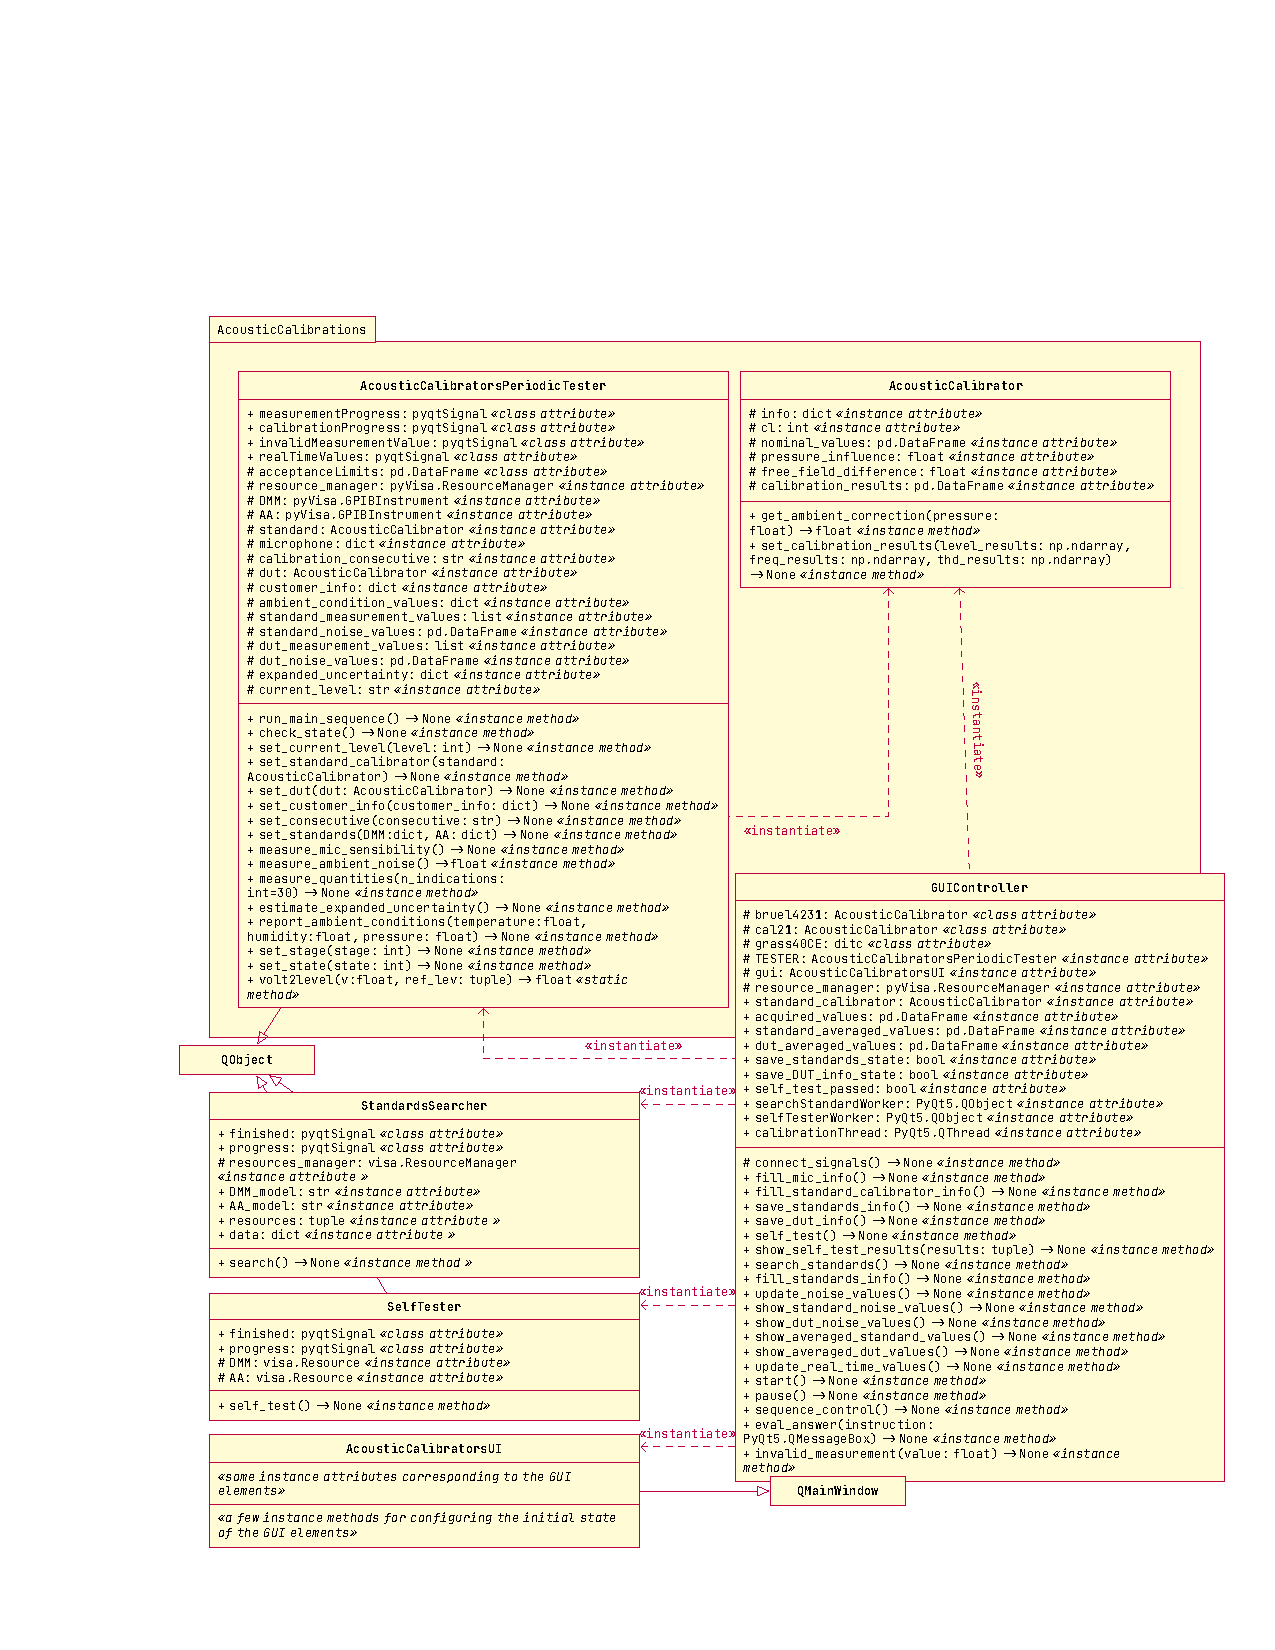
\includegraphics[width=\textwidth]{4_Implementación/IEC60942uml}
    \caption*{\footnotesize Fuente: Elaboración propia.}
\end{figure}

\subsubsection{Arquitectura de software}
%
El diagrama de clases de la figura~\ref{fig:uml_acoustic_calibrators} es un resumen de las clases principales (con sus atributos y métodos) diseñadas para el desarrollo de la aplicación para la calibración de calibradores acústicos.
También se presentan las clases heredadas y el instanciamiento entre clases.

La escritura del código se hizo aplicando las buenas prácticas de programación como: Documentación de clases, métodos e instrucciones relevantes, uso de atributos o métodos protegidos y las directrices de la guía PEP 8.
La interfaz gráfica se diseñó en Qt Designer de tal forma que se logre un manejo intuitivo de las funciones de la aplicación usando diferentes recursos como íconos, barras de progreso, menús desplegables, barra de herramientas, etc.
Con Qt Designer fue posible generar el código base de Python para el \emph{view} que lanza la aplicación y muestra la interfaz tal como fue diseñada.

\subsubsection{Descripción de funcionamiento}
\begin{figure}[!hb]
    \centering
    \caption{Interfaz gráfica de usuario de la aplicación para calibradores acústicos. Se muestra la pestaña de \emph{Patrones}.}
    \label{fig:calibrator_gui_standards}
    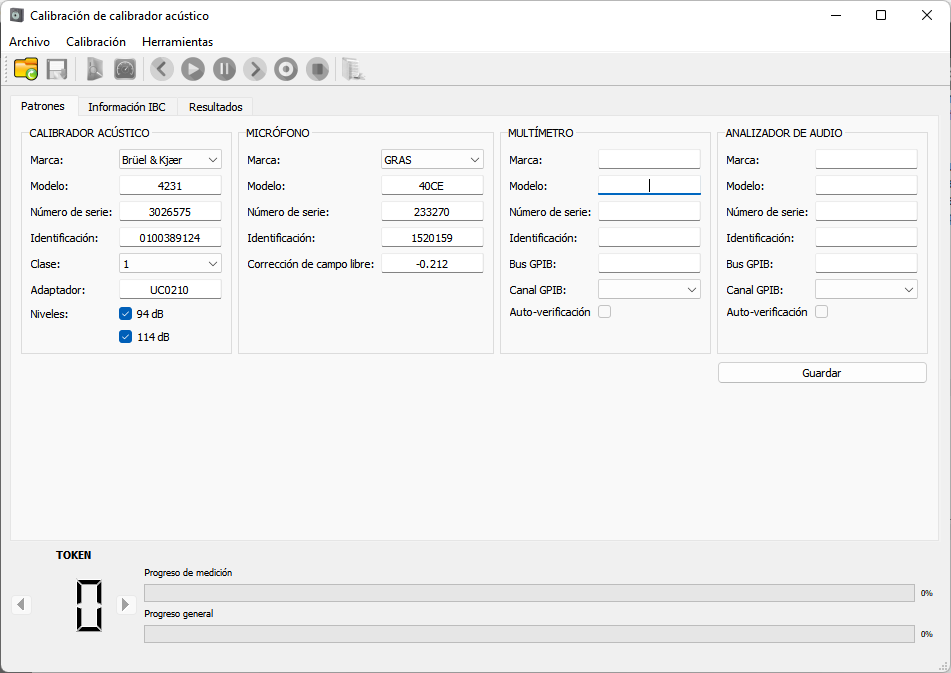
\includegraphics[width=0.8\textwidth]{4_Implementación/Figs/calibrator_gui_standards}
    \caption*{\footnotesize Fuente: Elaboración propia.}
\end{figure}
%
En la figura~\ref{fig:calibrator_gui_standards} se muestra la interfaz de usuario diseñada.
La pestaña de \emph{Patrones} es la mostrada en la vista inicial.
En esta, el usuario ingresa la información básica de los patrones empleados en la calibración.
Para el multímetro y el analizador de audio, si el usuario digita información en los campos de modelo, se habilita la herramienta 
\includegraphics[height=12pt]{4_Implementación/Figs/searchInstruments}, la cual busca automáticamente los modelos indicados entre todos los equipos disponibles conectados por GPIB al computador, extrae la información de estos y rellena los campos faltantes.

Una vez la información de los patrones está completa, el usuario puede hacer clic en \emph{Guardar}.
Se habilita la herramienta 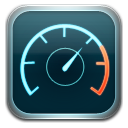
\includegraphics[height=12pt]{4_Implementación/Figs/test}, con la que se ejecuta la secuencia de auto-verificación de los patrones conectados por GPIB, si está disponible.
El resultado de la verificación se muestra en el \emph{check box} correspondiente.

\begin{figure}[!h]
    \centering
    \caption{Interfaz gráfica de usuario de la aplicación para calibradores acústicos. Se muestra la pestaña de \emph{Información IBC}.}
    \label{fig:calibrator_gui_dut}
    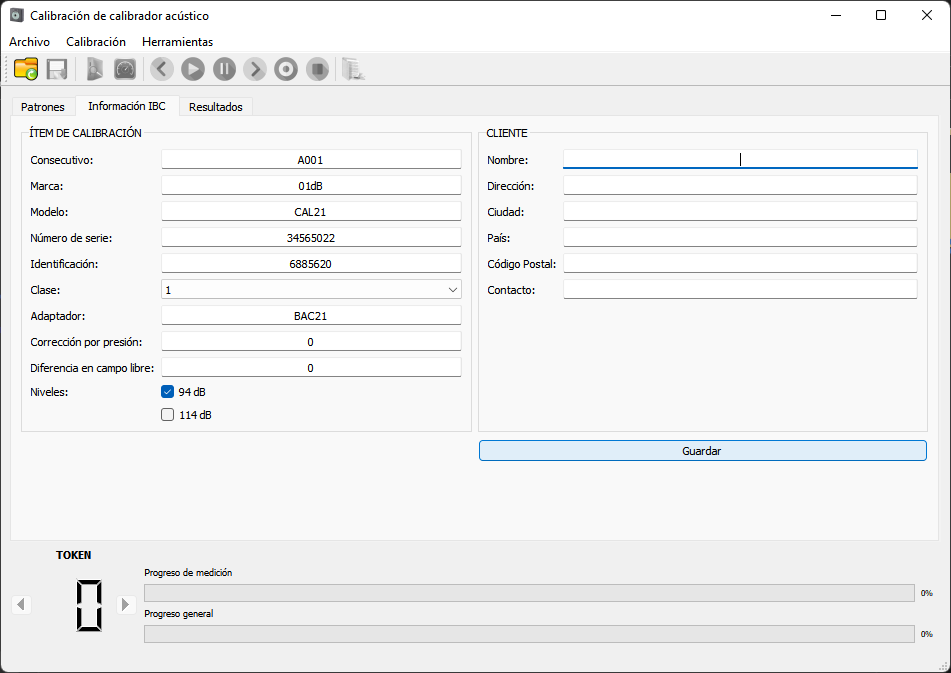
\includegraphics[width=0.8\textwidth]{4_Implementación/Figs/calibrator_gui_dut}
    \caption*{\footnotesize Fuente: Elaboración propia.}
\end{figure}

A continuación, en la pestaña \emph{Información IBC} (ver figura~\ref{fig:calibrator_gui_dut}), el usuario ingresa toda la información del calibrador bajo verificación y del cliente, necesaria para la calibración y para el certificado de calibración.
Cuando la información esté completa, el usuario puede hacer clic en \emph{Guardar} y, si el resultado de auto-verificación de los patrones fue correcto, entonces se habilita el botón 
\includegraphics[height=12pt]{4_Implementación/Figs/play}.
Al hacer clic en este se cumple la condición para la transición desde la etapa $0$ a la $1$ de la rutina principal del GRAFCET (figura~\ref{fig:GRAFCET_principal}).
En seguida se llevan a cabo todas las acciones de las demás etapas y, en la medida que avanza la secuencia, se van mostrando instrucciones al usuario para las acciones manuales y los resultados se presentan en tiempo real en la pestaña \emph{Resultados} (ver figura~\ref{fig:calibrator_gui_results}).

\begin{figure}[!h]
    \centering
    \caption{Interfaz gráfica de usuario de la aplicación para calibradores acústicos. Se muestra la pestaña de \emph{Resultados}.}
    \label{fig:calibrator_gui_results}
    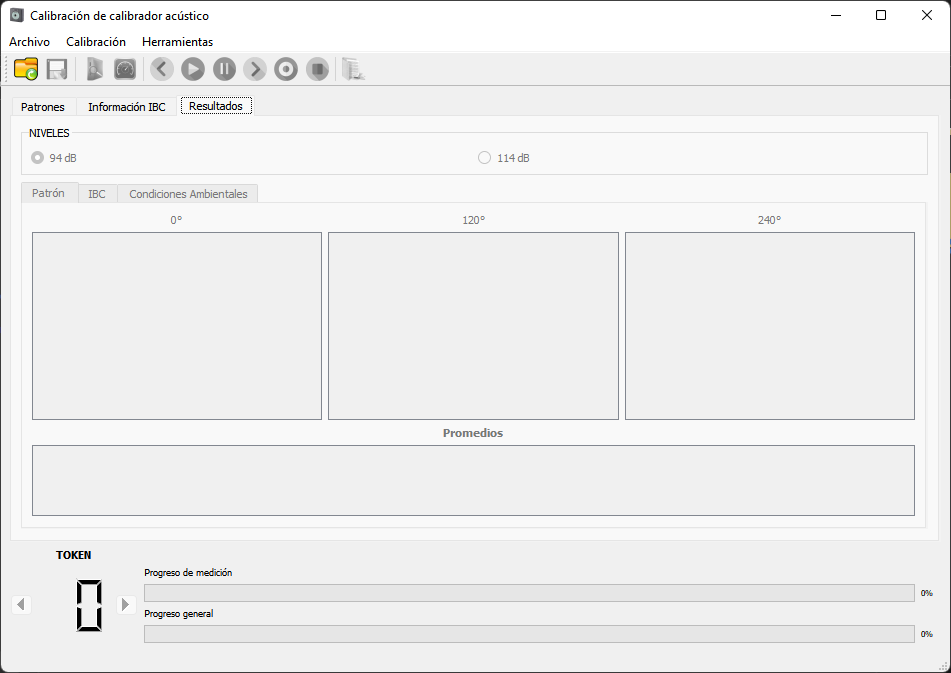
\includegraphics[width=0.8\textwidth]{4_implementación/Figs/calibrator_gui_results}
    \caption*{\footnotesize Fuente: Elaboración propia.}
\end{figure}

En la parte inferior de la ventana se incluye una barra de estado que indica la etapa actual (que tiene el \emph{token}), y dos barras de progreso, una para el progreso general de la calibración y otra para la medición en la etapa actual.
En cualquier momento de la calibración se puede hacer clic en 
\includegraphics[height=12pt]{4_Implementación/Figs/pause} para suspender temporalmente la secuencia y luego reanudarla haciendo clic nuevamente en 
\includegraphics[height=12pt]{4_Implementación/Figs/play}.
También se incluyeron en la interfaz otros botones y herramientas proyectando la aplicación a un desarrollo posterior que permita abrir y guardar sesiones de calibración, avanzar, retroceder etapas o ir a alguna específica del GRAFCET, y hasta generar automáticamente el certificado de calibración.


\section{Automatización de la calibración periódica de sonómetros}

De acuerdo con el método descrito en la sección~\ref{subsec:slm_calibration_description} y el diagrama de bloques de la figura~\ref{fig:slm_calibration_flowchart}, la aplicación se desarrolló con una metodología similar a la implementada para calibradores acústicos, como se explica en la siguiente sección.

\subsection{Implementación en Python}
El funcionamiento de la aplicación para calibradores acústicos asentó las bases para diseñar la aplicación para sonómetros.
Para aprovechar esas interacciones de los paradigmas \emph{model-view-controller} y GRAFCET que ocurren en el ambiente multihilos, se establecieron los siguientes pasos para la automatización de las pruebas realizadas en sonómetros;
estos pasos serían análogos a las etapas de un GRAFCET\@.

\begin{algorithm}[H]
    \caption{Pasos para la calibración periódica de sonómetros implementados en la aplicación desarrollada.}
    \label{alg:slm_calibration_steps}
    \scriptsize
    \DontPrintSemicolon
    \textbf{Paso 0.} Inicio, entrenar clasificador bayesiano. \;
    \textbf{Paso 1.} Verificar fuente de alimentación.\;
    \textbf{Paso 2.} Realizar prueba de indicación a la frecuencia de comprobación de la calibración.\;
    \textbf{Paso 3.} Verificar fuente de alimentación.\;
    \textbf{Paso 4.} Determinar el voltaje que produce una indicación del nivel de referencia.\;
    \textbf{Paso 5.} Realizar prueba de ponderación frecuencial $A$ con señales eléctricas.\;
    \textbf{Paso 6.} Realizar prueba de ponderación frecuencial $C$ con señales eléctricas.\;
    \textbf{Paso 7.} Realizar prueba de ponderación frecuencial $Z$ con señales eléctricas.\;
    \textbf{Paso 8.} Realizar prueba de ponderaciones frecuenciales a $\qty{1}{\kHz}$.\;
    \textbf{Paso 9.} Realizar prueba de ponderaciones temporales a $\qty{1}{\kHz}$.\;
    \textbf{Paso 10.} Realizar prueba de linealidad en el rango de niveles de referencia.\;
    \textbf{Paso 11.} Verificar fuente de alimentación.\;
    \textbf{Paso 12.} Fin\;
\end{algorithm}

%\begin{description}
%\item[Paso 0.] Inicio
%\item[Paso 1.] Verificar fuente de alimentación.
%\item[Paso 2.] Realizar prueba de indicación a la frecuencia de comprobación de la calibración.
%\item[Paso 3.] Verificar fuente de alimentación.
%\item[Paso 4.] Determinar el voltaje que produce una indicación del nivel de referencia.
%\item[Paso 5.] Realizar prueba de ponderación frecuencial $A$ con señales eléctricas.
%\item[Paso 6.] Realizar prueba de ponderación frecuencial $C$ con señales eléctricas.
%\item[Paso 7.] Realizar prueba de ponderación frecuencial $Z$ con señales eléctricas.
%\item[Paso 8.] Realizar prueba de ponderaciones frecuenciales a $\qty{1}{\kHz}$.
%\item[Paso 9.] Realizar prueba de ponderaciones temporales a $\qty{1}{\kHz}$.
%\item[Paso 10.] Realizar prueba de linealidad en el rango de niveles de referencia.
%\item[Paso 11.] Verificar fuente de alimentación.
%\item[Paso 12.] Fin
%\end{description}

Además de los hilos en los que el modelo hace sus operaciones y la vista envía y recibe las instrucciones del controlador, para esta aplicación fueron necesarios dos hilos más: uno que captura y muestra las imágenes del objeto de vídeo y otro que en segundo plano procesa, reconoce y guarda en disco en formato binario las imágenes de cada punto de calibración.
Todo esto a la vez que el modelo está corriendo temporizadores, enviando instrucciones a los instrumentos patrones y haciendo cálculos.
También se agregan otras señales Qt para indicar el arranque y parada de temporizadores, entregar el cuadro de vídeo capturado, indicar la liberación del objeto de vídeo y la finalización de guardado del vídeo, y enviar los mensajes de \emph{logging}.

Asignar los procesos de cálculo de los voltajes de prueba y temporizadores que se realizan en el modelo, y los procesos de reconocimiento de imágenes a hilos separados es un beneficio para el mantenimiento del \emph{software} y el desempeño de la aplicación.
Por ejemplo, el último objetivo de este proyecto, que consiste en el modelamiento de las cadenas de Markov, se puede implementar como un proceso adicional en el hilo de reconocimiento de imágenes, sin afectar los otros procesos.

\vfill

\begin{figure}[!hp]
    \caption{Diagrama de clases de la aplicación desarrollada para la calibración periódica de sonómetros.}
    \label{fig:uml_sonometers}
    \centering
    \includegraphics[width=\textwidth]{4_Implementación/IEC61672uml}
    \caption*{\footnotesize Fuente: Elaboración propia.}
\end{figure}
%
\begin{figure}[!h]
    \ContinuedFloat
    \centering
    \caption{Diagrama de clases de la aplicación desarrollada para la calibración periódica de sonómetros. (Continuación)}
    \begin{tikzpicture}[font=\tiny\ttfamily]
        \begin{class}[text width=1.6cm]{QMainWindow}{-1,0.9}\end{class}

        \begin{class}[text width=8cm]{SoundLevelMetersUI}{-1,0}
            \inherit{QMainWindow}
            \attribute{\textit{\guillemotleft some instance attributes corresponding to the GUI elements\guillemotright}}
            \operation{\textit{\guillemotleft a few instance methods for configuring the initial state of the GUI elements\guillemotright}}
        \end{class}

        \begin{class}[text width=4cm]{GUIController}{8,0}
            \attribute{\textit{\guillemotleft same attributes\guillemotright}}
            \operation{\textit{\guillemotleft same methods\guillemotright}}
        \end{class}

        \node (ACUINorth1)[below=0.2 of SoundLevelMetersUI.north east, inner sep=0pt, minimum size=0pt]{};
        \node (GUICWest4)[right=2.6 of ACUINorth1, inner sep=0pt, minimum size=0pt]{};
        \draw [umlcd style dashed line, <-] (ACUINorth1) -- node[pos=0.5,above,sloped]{\guillemotleft instantiate\guillemotright} (GUICWest4);

        \begin{class}[text width=2cm]{QObject}{-3,-4.5}\end{class}

        \begin{class}[text width=6cm]{VideoObject}{2, -2}
            \inherit{QObject}
            \attribute{+ frameCaptured: pyqtSignal \textit{\guillemotleft class attribute\guillemotright}}
            \attribute{+ cameraReleased: pyqtSignal \textit{\guillemotleft class attribute\guillemotright}}
            \attribute{+ loggingMsg: pyqtSignal \textit{\guillemotleft class attribute\guillemotright}}
            \attribute{+ run\_flag: bool \textit{\guillemotleft instance attribute\guillemotright}}
            \attribute{+ fps: int \textit{\guillemotleft instance attribute\guillemotright}}
            \attribute{+ frame\_size: tuple \textit{\guillemotleft instance attribute\guillemotright}}

            \operation{+ run() ->\,None \textit{\guillemotleft instance method\guillemotright}}
        \end{class}

        \begin{class}[text width=6cm]{VideoSaving}{2, -4.9}
            \inherit{QObject}
            \attribute{+ videoSaved: pyqtSignal \textit{\guillemotleft class attribute\guillemotright}}
            \attribute{+ loggingMsg: pyqtSignal \textit{\guillemotleft class attribute\guillemotright}}
            \attribute{+ frames: list \textit{\guillemotleft instance attribute\guillemotright}}
            \attribute{+ video\_writer: cv.VideoWriter \textit{\guillemotleft instance attribute\guillemotright}}

            \operation{+ save\_video() ->\,None \textit{\guillemotleft instance method\guillemotright}}
        \end{class}

        \begin{class}[text width=2cm]{QThread}{-3,-9}\end{class}

        \begin{class}[text width=6cm]{ImageProcessingThread}{2, -7.5}
            \inherit{QThread}
            \attribute{+ realTimeValues: pyqtSignal \textit{\guillemotleft class attribute\guillemotright}}
            \attribute{+ loggingMsg: pyqtSignal \textit{\guillemotleft class attribute\guillemotright}}
            \attribute{\# frames\_queue: Queue \textit{\guillemotleft instance attribute\guillemotright}}
            \attribute{\# TESTER: SLMPeriodicTester \textit{\guillemotleft instance attribute\guillemotright}}
            \attribute{\# stage: int \textit{\guillemotleft instance attribute\guillemotright}}
            \attribute{\# current\_f: int \textit{\guillemotleft instance attribute\guillemotright}}
            \attribute{\# fweightings: list \textit{\guillemotleft instance attribute\guillemotright}}
            \attribute{\# octave\_frequencies: list \textit{\guillemotleft instance attribute\guillemotright}}
            \attribute{+ fps: int \textit{\guillemotleft instance attribute\guillemotright}}

            \operation{+ run() ->\,None \textit{\guillemotleft instance method\guillemotright}}
        \end{class}

        \draw [umlcd style dashed line, <-](VideoObject.east) -| node[pos=0.3,above,sloped]{\guillemotleft instantiate\guillemotright} (GUIController.south);
        \draw [umlcd style dashed line, <-](VideoSaving.east) -| node[pos=0.3,above,sloped]{\guillemotleft instantiate\guillemotright} (GUIController.south);
        \draw [umlcd style dashed line, <-](ImageProcessingThread.east) -| node[pos=0.3,above,sloped]{\guillemotleft instantiate\guillemotright} (GUIController.south);
    \end{tikzpicture}
    \caption*{\footnotesize Fuente: Elaboración propia.}
\end{figure}

\subsubsection{Arquitectura de software}
El diagrama de clases de la figura~\ref{fig:uml_sonometers} es un resumen de las clases principales (con sus atributos y métodos) diseñadas para el desarrollo de la aplicación para la calibración de sonómetros.
También se presentan las clases heredadas y el instanciamiento entre clases.

La escritura del código se hizo aplicando las buenas prácticas de programación como: Documentación de clases, métodos e instrucciones relevantes, uso de atributos o métodos protegidos, aseguramiento de recursos para evitar condiciones de carrera entre hilos, colas para el procesamiento en segundo plano y las directrices de la guía PEP 8.
La interfaz gráfica se diseñó en Qt Designer de tal forma que se logre un manejo intuitivo de las funciones de la aplicación usando diferentes recursos como íconos, barras de progreso, menús desplegables, barra de herramientas, etc.
Con Qt Designer fue posible generar el código base de Python para el \emph{view} que lanza la aplicación y muestra la interfaz tal como fue diseñada.

\subsubsection{Descripción de funcionamiento}

\begin{figure}[!h]
    \centering
    \caption{Interfaz gráfica de usuario de la aplicación para sonómetros. Se muestra la pestaña de \emph{Patrones}.}
    \label{fig:slm_gui_standards}
    \includegraphics[width=\textwidth]{4_implementación/Figs/slm_gui_standards}
    \caption*{\footnotesize Fuente: Elaboración propia.}
\end{figure}

La aplicación para la calibración de sonómetros tiene un flujo de trabajo similar a la de calibradores acústicos.
En la figura~\ref{fig:slm_gui_standards} se muestra la interfaz gráfica de usuario diseñada.
En la vista inicial, la pestaña de \emph{Patrones} es la primera en mostrarse.
En esta, el usuario ingresa la información básica de los patrones empleados en la calibración.
Para el generador de señales y el multímetro digital, si el usuario digita información en los campos de modelo, se habilita la herramienta \includegraphics[height=12pt]{4_Implementación/Figs/searchInstruments}, la cual busca automáticamente los modelos indicados entre todos los equipos disponibles conectados por GPIB al computador, extrae la información de estos y rellena los campos faltantes.

Una vez la información de los patrones está completa, el usuario puede hacer clic en \emph{Guardar}.
Se habilita la herramienta \includegraphics[height=12pt]{4_Implementación/Figs/test}, con la que se ejecuta la secuencia de auto-verificación de los patrones conectados por GPIB, si está disponible.
El resultado de la verificación se muestra en el \emph{check box} correspondiente.

Dado que en esta aplicación se realizan más tareas y hay mayor interacción de los hilos de programación, fue conveniente incluir un {\footnotesize \texttt{QListWidget}} en el que se indexan registros de eventos con su correspondiente marca de tiempo, usando un código de colores (negro: mensaje informativo, verde: acción importante realizada y rojo: error o acción finalizada incorrectamente).
Este registro de eventos está siempre visible debajo del recuadro al que se transmiten los cuadros de vídeo.

\begin{figure}[!h]
    \centering
    \caption{Interfaz gráfica de usuario de la aplicación para sonómetros. Se muestra la pestaña de \emph{Información del IBC}.}
    \label{fig:slm_gui_dut}
    \includegraphics[width=\textwidth]{4_implementación/Figs/slm_gui_dut}
    \caption*{\footnotesize Fuente: Elaboración propia.}
\end{figure}

A continuación, en la pestaña \emph{Información IBC} (véase figura~\ref{fig:slm_gui_dut}), el usuario ingresa toda la información del sonómetro bajo verificación y del cliente, necesaria para la calibración y para el certificado de calibración.
Cuando la información esté completa, el usuario puede hacer clic en \emph{Guardar}.
Según la configuración indicada para el sonómetro, el programa buscará en una base de datos los factores de corrección de campo libre;
si estos no están disponibles, entonces el usuario puede crear un archivo separado por comas con los factores de corrección y cargarlos manualmente.
Luego, si el resultado de auto-verificación de los patrones fue correcto, entonces se habilita el botón \includegraphics[height=12pt]{4_Implementación/Figs/play}.
Al hacer clic en este se ejecuta el paso $0$ del algoritmo~\ref{alg:slm_calibration_steps}.
En seguida se llevan a cabo todas las acciones de los demás pasos y, en la medida que avanza la secuencia, se van mostrando instrucciones al usuario para las acciones manuales (ver figura~\ref{fig:slm_gui_results1}).

\vfill
\clearpage

\begin{figure}[!h]
    \centering
    \caption{Interfaz gráfica de usuario de la aplicación para sonómetros. Se muestra la pestaña de \emph{Pruebas preliminares} y un cuadro de diálogo con una instrucción.}
    \label{fig:slm_gui_results1}
    \includegraphics[width=0.9\textwidth]{4_implementación/Figs/slm_gui_results1}
    \caption*{\footnotesize Fuente: Elaboración propia.}
\end{figure}

\begin{figure}[!h]
    \centering
    \caption{Interfaz gráfica de usuario de la aplicación para sonómetros. Se muestra la pestaña de \emph{Pruebas preliminares} y la selección del área de interés sobre el vídeo.}
    \label{fig:slm_gui_results2}
    \includegraphics[width=0.9\textwidth]{4_implementación/Figs/slm_gui_results2}
    \caption*{\footnotesize Fuente: Elaboración propia.}
\end{figure}

\vfill
\clearpage

Al llegar al paso 5 (ponderación frecuencial $A$ con señales eléctricas), si no se ha activado la transmisión de vídeo, entonces esta iniciará y el usuario puede seleccionar el área de interés donde se encuentra el valor de medición que se desea reconocer (véase figura~\ref{fig:slm_gui_results2}).
Igualmente con las siguientes pruebas hasta el paso 10.
En la medida que avanzan las pruebas, los voltajes y frecuencias de las señales eléctricas se van ajustando automáticamente y se muestran en el historial los comandos SCPI enviados;
los resultados se presentan en tiempo real en sus campos correspondientes según la prueba en curso como se muestra en la siguiente figura.

\begin{figure}[!h]
    \centering
    \caption{Interfaz gráfica de usuario de la aplicación para sonómetros. Se muestra la pestaña de \emph{Ponderaciones frecuenciales y temporales} y la presentación de resultados.}
    \label{fig:slm_gui_results3}
    \includegraphics[width=\textwidth]{4_implementación/Figs/slm_gui_results3}
    \caption*{\footnotesize Fuente: Elaboración propia.}
\end{figure}

\vfill
\clearpage
%  ╔═╗┌─┐┌┬┐┌─┐┌┐┌┌─┐┌─┐  ┌┬┐┌─┐  ╔╦╗┌─┐┬─┐┬┌─┌─┐┬  ┬
%  ║  ├─┤ ││├┤ │││├─┤└─┐   ││├┤   ║║║├─┤├┬┘├┴┐│ │└┐┌┘
%  ╚═╝┴ ┴─┴┘└─┘┘└┘┴ ┴└─┘  ─┴┘└─┘  ╩ ╩┴ ┴┴└─┴ ┴└─┘ └┘ 

\chapter{Caracterización de la variabilidad del valor de medición usando modelos de Markov}

En esta sección se explica el diseño e implementación del método propuesto para tener en cuenta la variabilidad del nivel indicado en la pantalla del sonómetro bajo calibración en el resultado de medición, expresado como el valor de medición junto con la incertidumbre expandida de medición.
En primer lugar, se describen las consideraciones previas que dan validez al método propuesto y se introduce el algoritmo que resume la ejecución del método en una serie de pasos.
Luego, se presenta el fundamento teórico suficiente de los procesos estocásticos modelados con cadenas de Markov y se describen brevemente los detalles de la implementación del método.
Finalmente, se muestra y discute un ejemplo de un valor de medición obtenido con el método implementado y su correspondiente incertidumbre de medida tipo A\@.

\section*{Consideraciones previas}
El nivel instantáneo ponderado en tiempo y en frecuencia definido en la ecuación~\eqref{eq:time_weighted_level} no es un indicador representativo del nivel de sonidos cuya presión tiene bastante variabilidad, ya que es muy susceptible a las variaciones instantáneas en la presión acústica, por lo que normalmente en mediciones acústicas se evalúa el nivel de sonido promediado en el tiempo o nivel de sonido continuo equivalente, definido en la \mbox{IEC 61672--1}~\citeyearpar{IEC_TC29_2013_1} como
%
\begin{equation}
    \label{eq:equivalent_level}
    L_{Xeq,T} = 10\log{\left(\frac{\frac{1}{t_1 - t_2}\,\int_{t_2}^{t_1} p_X^2\left(\xi\right)\,\mathrm{d}\xi}{p_0^2}\right)},
\end{equation}
%
En que $t_1$ y $t_2$ son el instante de tiempo final e inicial de integración correspondientemente.
El nivel continuo equivalente es un indicador mucho más confiable, ya que se trata de un nivel constante que, durante todo el tiempo de integración, tiene la misma energía acústica que la señal de presión con sus variaciones instantáneas.

Ahora, medir el nivel equivalente requiere una intervención manual del usuario para ajustar en el sonómetro el tiempo de integración y ver el resultado final, por lo que este indicador no es el más adecuado para la automatización empleando reconocimiento de imágenes.
No obstante, la \mbox{IEC 61672--3}~\citeyearpar{IEC_TC29_2013_3} permite seleccionar entre un nivel ponderado en el tiempo o un nivel promediado en el tiempo, como valor de medición en cada punto de calibración.
Para no comprometer la automatización y obtener un resultado de medición válido y representativo de todas las posibles variaciones que pueda tener el nivel instantáneo ponderado en el tiempo, se propone tener en cuenta todas las muestras del nivel ponderado en el tiempo y luego, el nivel presente en la mayor cantidad de muestras viene a ser una estimación apropiada del nivel promediado en el tiempo (esto en condiciones controladas, como es el caso en laboratorios de calibración).
Este efecto se puede comprobar analizando las expresiones matemáticas de cada indicador.
En primer lugar, de la ecuación~\eqref{eq:time_weighted_level} se extrae que la presión acústica con ponderación temporal, expresada como una función del tiempo es
%
\begin{equation}
    p_{XY}^2(t) = \frac{1}{\tau_{Y}}\,\int_{-\infty}^t p_X^2\left(\xi\right)\,
    e^{\nicefrac{-\left(t - \xi\right)}{\tau_Y}}\,\mathrm{d}\xi.
\end{equation}

Esta presión instantánea ponderada en el tiempo no es la misma de la ecuación~\eqref{eq:equivalent_level}.
Para calcular un nivel continuo equivalente con ponderación temporal y frecuencial se requiere modificar la ecuación~\eqref{eq:equivalent_level} remplazando $p_X^2(\xi)$ por $p_{XY}^2(t)$; en efecto, queda
%
\begin{align}
    L_{AFeq,T} &= 10\log{\left(\frac{\frac{1}{t_1 - t_2}\,\int_{t_2}^{t_1} p_{XY}^2(t)\,\mathrm{d}t}{p_0^2}\right)}; \nonumber \\
    &= 10\log{\left(\frac{\frac{1}{\tau_Y\,\left(t_1 - t_2\right)}\,
    \int_{t_2}^{t_1} \int_{-\infty}^t p_X^2\left(\xi\right)\,
    e^{\nicefrac{-\left(t - \xi\right)}{\tau_Y}}\,\mathrm{d}\xi\,\mathrm{d}t}{p_0^2}\right)}. \label{eq:equivalent_time_weighted_level}
\end{align}

En la ecuación~\eqref{eq:equivalent_time_weighted_level} se puede concluir que cuanto más tiempo permanezca estable una presión acústica instantánea ponderada en tiempo, el nivel equivalente más se acercará al correspondiente nivel instantáneo ponderado en tiempo, pues tiene mayor efecto en el resultado de la integral.

\section*{Algoritmo para la creación del modelo de Markov}
El método propuesto consiste en tomar cada uno de los niveles instantáneos obtenidos como un estado en una cadena de Markov.
Esta cadena caracteriza los cambios de un nivel a otro, considerando la variabilidad del nivel instantáneo como un proceso estocástico.
Luego, con la distribución de probabilidad estacionaria se estima el valor esperado en el largo plazo, que lógicamente corresponde al estado (nivel instantáneo) con mayor probabilidad de ocurrir.
Las probabilidades de transición de un estado a otro se determinan a partir de una serie de muestras de niveles instantáneos obtenidas durante un tiempo de $25$ segundos aproximadamente, y la cantidad de muestras depende del periodo de actualización del nivel instantáneo en la pantalla del sonómetro.
Por tanto, el valor esperado calculado con la cadena de Markov será probablemente el nivel instantáneo que más muestras tuvo y será el valor de medición.
Este es un proceso que se realiza en cada punto de calibración y se resume en el siguiente algoritmo, y las operaciones realizadas en cada paso, se describen en las siguientes secciones.

\begin{algorithm}[H]
    \caption{Algoritmo para el cálculo del valor esperado usando cadenas de Markov.}
    \label{alg:markov_expected_value}
    \scriptsize
    \DontPrintSemicolon
    \SetKwData{frames}{frames}
    \SetKwInOut{Output}{output}
    \KwData{\frames $\leftarrow$ \text{Vídeo de $\qty{25}{\s}$ del nivel instantáneo indicado en pantalla.}}
    \Output{Valor esperado}
    \BlankLine
    \textbf{\hyperref[sec:downsampling]{Paso 1}:} Submuestrear y reconocer cuadros después del tiempo de estabilización.\;
    \textbf{\hyperref[subsec:transition_matrix]{Paso 2}:} Conformar matriz de transición de estados.\;
    \textbf{\hyperref[subsec:stationary_distribution]{Paso 3}:} Calcular distribución de probabilidad estacionaria.\;
    \textbf{\hyperref[sec:fill_missing_values]{Paso 4}:} Completar valores faltantes usando la matriz de transición.\;
    Repetir paso 2.\;
    Repetir paso 3.\;
    \textbf{\hyperref[subsec:expected_value]{Paso 5}:} Calcular valor esperado.\;
\end{algorithm}

\section*{Paso 1: Submuestreo y reconocimiento de cuadros después de la estabilización}
\label{sec:downsampling}
Como el nivel con ponderación temporal \emph{Fast}, que tiene una constante de tiempo $\tau_F = \qty{125}{\ms}$, requiere un tiempo transitorio hasta que el nivel se estabilice después de enviar la señal eléctrica.
Se determinó experimentalmente un tiempo de $\qty{2}{\s}$.
Los cuadros obtenidos durante este tiempo de estabilización no se tienen en cuenta para la matriz de transición, pero sí para determinar el cuadro $0$ para sincronizar la actualización del nivel instantáneo en pantalla con los cuadros del vídeo.

Para determinar el cuadro $0$ primero se efectúa el algoritmo~\ref{alg:image_recongnition} en los cuadros del tiempo de estabilización.
Con el vector de los valores numéricos reconocidos se encuentra el índice del primer cambio de valor.
Luego, a los cuadros después de ese índice se les hace un submuestreo según la relación entre la tasa de cuadros por segundo de la cámara y la tasa de actualización de la pantalla del sonómetro.
Los cuadros que quedan corresponden al instante exacto en el que hay una nueva muestra en pantalla.
Sin embargo, dado que puede presentarse en la pantalla LCD un efecto de solapamiento entre la muestra anterior y la nueva, que afecta negativamente el reconocimiento de imágenes, se determinó experimentalmente tomar $4$ cuadros después del cuadro en el que ocurre el cambio, para permitir la estabilización de la pantalla.

En seguida, en el nuevo vector de cuadros submuestreado se busca el índice del cuadro inmediatamente después al tiempo de estabilización, que corresponde al producto del tiempo de estabilización y la tasa de actualización de la pantalla del sonómetro.
Finalmente, se efectúa el reconocimiento de los cuadros submuestreados a partir del índice del cuadro de estabilización con el algoritmo~\ref{alg:image_recongnition}.
El vector de valores numéricos reconocidos es el arreglo de muestras a partir del cual se conforma la matriz de transición de estados en el paso a continuación.


\section{Cadenas de Markov de tiempo discreto}

\subsection*{Paso 2: Matriz de probabilidades de transición}
\label{subsec:transition_matrix}
Tomando como guía el libro de Robert Dobrow~\citeyearpar{Dobrow2016} y el de John Gubner~\citeyearpar{Gubner2006}, una cadena de Markov es un proceso aleatorio con la propiedad particular de que, dados unos valores del proceso desde el tiempo cero hasta el tiempo actual, la probabilidad condicional del valor del proceso en algún tiempo futuro depende solo del valor actual, es decir, el futuro y el pasado son condicionalmente independientes dado el presente.
Analíticamente, una cadena de Markov es una secuencia de variables aleatorias $X_0, X_1, \dots$ que toman valores del espacio discreto de estados $\mathcal{S}$ con la propiedad de que
%
\begin{equation}
    \label{eq:markov_chain}
    P\left(X_{n + 1} = j\,|\,X_0 = x_0, \dots, X_{n - 1}
    = x_{n - 1}, X_n = i\right) = P\left(X_{n + 1} = j\,|\,X_n = i\right),
\end{equation}
%
Para todo $x_0, \dots, x_{n - 1}, i, j \in \mathcal{S}$ y $n \ge 0$.
Normalmente, se asume que todas las cadenas de Markov son homogéneas, en las que la probabilidad no depende de $n$.

En la ecuación~\eqref{eq:markov_chain} las probabilidades solamente dependen de $i$ y $j$, por lo que estas se pueden organizar de forma matricial en $\mathbf{P}$, cuya $ji$-ésima entrada es $p_{ij} = P\left(X_{n + 1} = j\,|\,X_n = i\right)$, la probabilidad de transición de un estado a otro en un paso.
La matriz de transición es una matriz cuadrada de $k \times k$ para los $k$ estados en el espacio $\mathcal{S}$.

\begin{code}
    \caption{Método estático para la construcción de una matriz de transición de estados a partir de una serie de muestras dada.}
    \label{code:build_transition_matrix}
    \centering
    \begin{minted}{python}
@staticmethod
def build_transition_matrix(samples: np.ndarray) -> np.ndarray:
    """
    Method for construction of the states transition matrix from a sequence of samples
    :param samples: A numpy one dimensional ndarray with the sequence of samples.
    :return: A numpy array that represents the transition matrix of the Markov model.
    """
    states = np.unique(samples)  # Remove repeated samples
    P = pd.DataFrame(data=np.zeros((states.shape[0], states.shape[0])), index=states, columns=states)  # Empty P
    for i in range(1, samples.shape[0]):  # Counts transitions from state to state
        P.loc[samples[i - 1], samples[i]] += 1
    P = P.div(P.sum(axis=1), axis=0)  # Computes probabilities
    return P
    \end{minted}
\end{code}

La matriz de transición o matriz estocástica debe cumplir que $p_{ij} \ge 0 \quad \forall\,i,j$ y que
%
\begin{equation*}
    \sum_j p_{ij} = \sum_j P\left(X_{n + 1} = j\,|\,X_n = i\right)
    = \sum_j \frac{P\left(X_{n + 1} = j, X_n = i\right)}{P\left(X_n = i\right)}
    = \frac{P\left(X_n = i\right)}{P\left(X_n = i\right)} = 1.
\end{equation*}
%
Lo que indica que las transiciones en las cadenas de Markov son exhaustivas.

Teniendo en cuenta este fundamento conceptual, para cada punto de calibración se conforma una matriz de transición en la que cada nivel diferente indicado en pantalla es un estado en la cadena de Markov.
Para este efecto se escribió el método estático del código~\ref{code:build_transition_matrix}.

\subsection*{Paso 3: Distribución de probabilidad estacionaria}
\label{subsec:stationary_distribution}
Una vez se conforma una matriz con las probabilidades de transición se puede usar álgebra matricial para hacer cálculos con las probabilidades.
Uno de los más elementales es el cálculo de las probabilidades de transición del estado $i$ al $j$ en $n \ge 1$ pasos, es decir $p_{ij}^{(n)} = P\left(X_n = j \,|\,X_0 = i\right)$, la probabilidad de que en $n$ pasos el proceso visite el estado $j$ dado que ahora está en el estado $i$.
Cuando $n = 1$ las probabilidades son las mismas de $\mathbf{P}$, pero cuando $n \ge 1$ las probabilidades de transición son los $ij$-ésimos elementos de la potencia $n$ de $\mathbf{P}$, denotada como $\mathbf{P}^n$.

Es de especial interés conocer el comportamiento del sistema en el largo plazo, lo cual está caracterizado por las potencias de mayor orden de $\mathbf{P}$.
En la medida en que $n$ incrementa, el proceso alcanza un comportamiento límite y las probabilidades de transición convergen a una distribución de equilibrio, conocida como distribución límite, la cual no depende de la distribución de probabilidad inicial de los estados.
Para una cadena de Markov la distribución límite es la distribución de probabilidad $\boldsymbol{\lambda}$ con la propiedad de que para todo $i$ y $j$
%
\begin{equation}
    \lim_{n\to\infty} P_{ij}^n = \lambda_{j}.
\end{equation}

Si una cadena de Markov tiene una distribución límite, entonces esta es única.
Se puede encontrar la distribución límite simplemente tomando las potencias de mayor orden hasta obtener una matriz $\boldsymbol{\Lambda}$ en la cual todas las filas son iguales a $\boldsymbol{\lambda}$, o también se pueden encontrar soluciones exactas de forma analítica y teórica.
Cabe mencionar que la distribución límite también puede ser interpretada como la proporción de tiempo que el proceso visita cada estado en el largo plazo

Ahora, si se asigna la distribución límite como la distribución inicial de la cadena de Markov, luego se encuentran las probabilidades marginales $\boldsymbol{\lambda}\,\mathbf{P}$, y el resultado es el mismo vector $\boldsymbol{\lambda}$, entonces esta distribución límite es llamada distribución estacionaria.
Es decir, una distribución estacionaria es una distribución de probabilidad $\boldsymbol{\pi}$ que satisface $\boldsymbol{\pi} = \boldsymbol{\pi}\,\mathbf{P}$, o lo que es igual
%
\begin{equation}
    \label{eq:stationary_distribution}
    \pi_j = \sum_i \pi_j\, P_{ij}, \quad \forall\, j.
\end{equation}

Aunque la distribución límite y la estacionaria están relacionadas, una cadena de Markov puede tener más de una distribución estacionaria o ninguna, y esta no necesariamente es la distribución límite.
Pero si la cadena tiene una distribución límite, entonces esa distribución es estacionaria.\ Esto depende directamente de la topología de la cadena;
si la cadena es regular entonces su matriz de transición $\mathbf{P}$ es regular (todos los valores de alguna de sus potencias son positivos), y la distribución límite es igual a la estacionaria.

Para encontrar la distribución estacionaria cuando la matriz es regular, la forma más directa es resolver el sistema lineal de ecuaciones que resulta de combinar la ecuación~\eqref{eq:stationary_distribution} y la restricción $\sum_i \pi_i = 1$.
La ecuación~\eqref{eq:stationary_distribution} puede escribirse matricialmente como $\boldsymbol{\pi}\,(\mathbf{P} - \mathbf{I}) = 0$, o, para operar con vectores columna, como $\left(\mathbf{P}^\intercal - \mathbf{I}\right)\,\boldsymbol{\pi} = 0$.
Finalmente, se puede escribir el sistema de ecuaciones matricialmente como
%
\begin{align}
    \mathbf{A}\,\boldsymbol{\pi} &= \mathbf{b}; \\
    \left[\begin{matrix}
              \left(\mathbf{P}^\intercal - \mathbf{I}\right) \\ 1 \\ \vdots \\ 1;
    \end{matrix}\right]\,\boldsymbol{\pi} &= \left[\begin{matrix}
                                                       0 \\ 0 \\ \vdots \\ 1
    \end{matrix}\right].
\end{align}

Para encontrar soluciones para $\boldsymbol{\pi}$ se resuelve el sistema
\begin{equation}
    \label{eq:pi_linear_system}
    \left(\mathbf{A}^\intercal\,\mathbf{A}\right)\,\boldsymbol{\pi} = \mathbf{A}^\intercal\,\mathbf{b}.
\end{equation}

Para implementar lo anterior y calcular la distribución límite dada una matriz de transición $\mathbf{P}$ se escribió el método estático del código~\ref{code:limit_dist}.

\subsection*{Paso 5: Valor esperado}
\label{subsec:expected_value}

En un sistema discreto, el valor esperado calculado a partir de la distribución estacionaria es
%
\begin{equation}
    \mathrm{E}[X] = \sum_n x_n\,\pi_n,
\end{equation}
%
Que puede implementarse simplemente como \mintinline{python}{expected_value = np.round(np.sum(np.array(P.index) * PI.T), 1)}.

\begin{code}
    \caption{Método estático para el cálculo de la distribución límite de una cadena de Markov dada una matriz de transición.}
    \label{code:limit_dist}
    \centering
    \begin{minted}{python}
def limit_dist(P: np.ndarray) -> float:
    """
    Method to calculate the limit distribution with linear algebra solution using a given transition matrix P if
    the given matrix is a regular matrix, else, the calculation is performed with the high matrix powers of the
    transition matrix.
    :param P: The numpy array that represents de transition matrix.
    :return: The stationary distribution as a float number.
    """
    for n in range(2, 1001):
        if np.all(np.linalg.matrix_power(P, n) > 0):  # Check if it is a regular transition matrix
            # The matrix is regular, so limiting distribution exists and is the unique stationary distribution
            A = np.append(np.transpose(P) - np.identity(P.shape[0]), np.ones((1, P.shape[0])),
                          axis=0)  # Augmented A
            b = np.zeros((A.shape[0], 1))
            b[-1] = 1  # Augmented b
            PI = np.linalg.solve(np.transpose(A).dot(A), np.transpose(A).dot(b))  # Stationary distribution
            break
    else:
        PI = np.linalg.matrix_power(P, 1000)

    return PI
    \end{minted}
\end{code}

\section*{Paso 4: Completar valores faltantes}
\label{sec:fill_missing_values}
Aún cuando el clasificador tiene un buen desempeño y el submuestreo se ha realizado evitando el efecto de solapamiento de valores en la pantalla del sonómetro, puede ocurrir que eventualmente un cuadro capturado coincide con la actualización del valor en pantalla y consecuentemente el clasificador devuelve un resultado incorrecto.
Para estos casos poco recurrentes, se determinó que el clasificador devolviera un valor \texttt{\small np.nan}.
Esta es una muestra faltante que debe ser completada para continuar con el proceso.

Para remplazar la muestra faltante conviene utilizar la matriz inicial de transición de un paso construida en el \hyperref[sec:downsampling]{Paso 1} para ubicar el valor más probable a partir del valor anterior.
En el caso en el que la primera muestra sea un estado faltante, esta se completa con la distribución estacionaria de la matriz de transición inicial.
Esto es razonable porque los valores ubicados obedecen a la dinámica del proceso estocástico que fue caracterizada en la matriz de transición inicial.
En efecto, este paso se realiza con el siguiente código.
%
\begin{code}
    \caption{Ciclo para completar muestras faltantes a partir del modelo inicial de Markov.}
    \label{code:filling_missing_samples}
    \centering
    \begin{minted}{python}
samples[0] = P.index[PI.argmax()] if np.isnan(samples[0]) else samples[0]  # If initial state is missing
for i in np.where(np.isnan(samples))[0]:  # Filling based on the previous state and the Markov model
    samples[i] = P.index[P.loc[samples[i - 1]].argmax()]
    \end{minted}
\end{code}

Una vez el vector de muestras está completo, se construye una segunda matriz de transición y nuevamente se calcula la distribución estacionaria que se empleará en el cálculo del valor esperado.

\begin{figure}[!h]
    \caption{Grafo de estados y probabilidades de transición que representa la matriz de transición~\eqref{eq:eg_transition_matrix}.}
    \label{fig:eg_automata}
    \centering
    \begin{tikzpicture}[thick,shorten >=1pt,node distance=6cm,on grid,auto]
        \node[state](q1){$\qty{33.1}{\dB}$};
        \node[state](q2)[below=of q1]{$\qty{33.2}{\dB}$};
        \node[state](q3)[right=of q1]{$\qty{33.3}{\dB}$};
        \node[state](q4)[below=of q3]{$\qty{33.4}{\dB}$};
        \draw[->, stealth-]
        (q1) edge [loop left] node {$\num{0.200}$} ()
        edge [bend right, swap] node {$\num{0.045}$} (q2)
        edge [swap] node {$\num{0.022}$} (q3)
        (q2) edge [loop left] node {$\num{0.455}$} ()
        edge [swap, pos=0.6] node {$\num{0.200}$} (q1)
        edge [bend right] node {$\num{0.696}$} (q3)
        edge [bend right, swap] node {$\num{0.667}$} (q4)
        (q3) edge [loop right] node {$\num{0.261}$} ()
        edge [bend right, swap] node {$\num{0.600}$} (q1)
        edge [bend right] node {$\num{0.455}$} (q2)
        edge [swap, pos=0.6] node {$\num{0.333}$} (q4)
        (q4) edge [swap] node {$\num{0.045}$} (q2)
        edge [bend right, swap] node {$\num{0.022}$} (q3);
    \end{tikzpicture}
    \caption*{\footnotesize Fuente propia.}
\end{figure}

\section{Ejemplo de resultado de ejecución del método}
Habiendo incluido apropiadamente este método en el desarrollo previo de la aplicación, se obtuvieron los resultados esperados.
Un ejemplo de una matriz de transición obtenida en la prueba de ponderación frecuencial $Z$ con señales eléctricas a $\qty{63}{\Hz}$ se muestra a continuación.
%
\begin{equation}
    \label{eq:eg_transition_matrix}
    \mathbf{P} = \kbordermatrix{
        & \mathbf{\num{33,1}} & \mathbf{\num{33.2}} & \mathbf{\num{33.3}} & \mathbf{\num{33.4}} \\
        \mathbf{\num{33.1}} & \num{0.200} & \num{0.200} & \num{0.600} & \num{0.000} \\
        \mathbf{\num{33.2}} & \num{0.045} & \num{0.455} & \num{0.455} & \num{0.045} \\
        \mathbf{\num{33.3}} & \num{0.022} & \num{0.696} & \num{0.261} & \num{0.022} \\
        \mathbf{\num{33.4}} & \num{0.000} & \num{0.667} & \num{0.333} & \num{0.000} \\
    }
\end{equation}
%
Y el grafo correspondiente se representa en la figura~\ref{fig:eg_automata}.

Resolviendo el sistema de la ecuación~\eqref{eq:pi_linear_system}, la distribución estacionaria es
%
\begin{equation*}
    \boldsymbol{\pi} = \kbordermatrix{
        & \mathbf{\num{33.1}} &  \mathbf{\num{33.2}} &  \mathbf{\num{33.3}} & \mathbf{\num{33.4}} \\
        & \num{0.041} & \num{0.543} & \num{0.382} & \num{0.033}
    }
\end{equation*}

Finalmente, el valor esperado, redondeado a la misma cantidad de dígitos decimales de la precisión del sonómetro es $\qty{33.2}{\dB}$.


\section{Evaluación tipo A de la incertidumbre típica}

De a cuerdo con la guía para la expresión de la incertidumbre de medida~\citep{ISO_TAG4_2008}, los valores de las observaciones individuales $q_k$ difieren en razón de las variaciones aleatorias de las magnitudes de influencia o de efectos aleatorios.
La varianza experimental de dichas $n$ observaciones está dada por:
%
\begin{equation}
    s^2\left( q_k \right) = \frac{1}{n - 1}\, \sum_{j = 1}^{n} \left( q_j - \bar{q} \right)^2,
\end{equation}
%
Que, junto con su raíz cuadrada positiva $s\left( q_k \right)$ (denominada desviación típica experimental), representan la variabilidad de los valores $q_k$, es decir, su dispersion al rededor del valor esperado $\bar{q}$.
Luego, la mejor estimación de la varianza experimental de la media $\sigma^2\left( \bar{q} \right) = \sigma^2 / n$ es
%
\begin{equation}
    \label{eq:experimental_mean_variance}
    s^2\left( \bar{q} \right) = \frac{s^2\left( q_k \right)}{n},
\end{equation}
Que, junto con desviación típica experimental de la media $s\left( \bar{q} \right) = \sqrt{s^2\left( \bar{q} \right)}$ pueden ser utilizadas como medida de la incertidumbre de $\bar{q}$.

En concreto, en un modelo matemático de un mesurando $y$, para una magnitud de entrada $X_i$ obtenida a partir de $n$ observaciones repetidas e independientes $X_{i,k}$, la incertidumbre típica $u\left( x_i \right)$ de su estimación $x_i = \bar{X}_i$ es $u\left( x_i \right) = s\left( \bar{X}_i \right)$, con $s^2\left( \bar{X}_i \right)$ calculada con la ecuación~\eqref{eq:experimental_mean_variance}.
Esta incertidumbre típica $u\left( x_i \right)$ es llamada \emph{incertidumbre típica tipo A}.

El número de observaciones $n$ debe ser lo suficientemente grande para garantizar que $s^2\left( \bar{q} \right)$ proporcione una estimación fiable de la varianza $\sigma^2\left( \bar{q} \right)$.
La aplicación desarrollada permite cumplir esta consideración, puesto que en un tiempo de $\qty{25}{\s}$, con un periodo de actualización de pantalla típico de $\qty{100}{\ms}$, se capturan $250$ muestras.
Ahora, en un cálculo posterior, cuando se determinan intervalos de confianza para la incertidumbre expandida, se debe tomar en cuenta la diferencia entre $\sigma^2\left( \bar{q} \right)$ y $s\left( \bar{q} \right)$, ya que en muchos casos puede ser que la distribución de probabilidad del mesurando (en este caso equivale a la distribución estacionaria) sea muy distinta de una distribución normal.

La estimación de la incertidumbre típica tipo A puede hacerse rápidamente con la instrucción \mintinline{python}{samples.std() / math.sqrt(samples.shape[0])}.
Para las muestras del ejemplo anterior se obtiene $s\left( \bar{q} \right) \approx \qty{0.0057}{\dB}$.
%  ╔═╗┌─┐┌┐┌┌─┐┬  ┬ ┬┌─┐┬┌─┐┌┐┌┌─┐┌─┐
%  ║  │ │││││  │  │ │└─┐││ ││││├┤ └─┐
%  ╚═╝└─┘┘└┘└─┘┴─┘└─┘└─┘┴└─┘┘└┘└─┘└─┘

\chapter{Conclusiones y recomendaciones}
\section{Conclusiones}
Las conclusiones constituyen un cap\'{\i}tulo independiente y presentan, en forma l\'{o}gica, los resultados de la tesis  o trabajo de investigaci\'{o}n. Las conclusiones deben ser la respuesta a los objetivos o prop\'{o}sitos planteados. Se deben titular con la palabra conclusiones en el mismo formato de los t\'{\i}tulos de los cap\'{\i}tulos anteriores (T\'{\i}tulos primer nivel), precedida por el numeral correspondiente (seg\'{u}n la presente plantilla).\\

\section{Recomendaciones}
Se presentan como una serie de aspectos que se podr\'{\i}an realizar en un futuro para emprender investigaciones similares o fortalecer la investigaci\'{o}n realizada. Deben contemplar las perspectivas de la investigaci\'{o}n, las cuales son sugerencias, proyecciones o alternativas que se presentan para modificar, cambiar o incidir sobre una situaci\'{o}n espec\'{\i}fica o una problem\'{a}tica encontrada. Pueden presentarse como un texto con caracter\'{\i}sticas argumentativas, resultado de una reflexi\'{o}n acerca de la tesis o trabajo de investigaci\'{o}n.\\
%  ╔═╗┌┐┌┌─┐─┐ ┬┌─┐┌─┐
%  ╠═╣│││├┤ ┌┴┬┘│ │└─┐
%  ╩ ╩┘└┘└─┘┴ └─└─┘└─┘

\begin{appendix}

\chapter{Anexo: Códigos de Python y subrutinas GRAFCET}

\begin{code}
	\caption{Código para presentar resultados del procesamiento de una muestra del número $5$ del conjunto de imágenes entrenamiento.}
	\label{code:test_samples_code}
	\centering
	\inputminted{python}{3_Reconocimiento/Codes/image_processing_test.py}
\end{code}

\begin{code}
	\caption{Código para realizar la extracción de características de los vectores de entrenamiento y para entrenar el clasificador.}
	\label{code:features_extracting}
	\centering
	\inputminted{python}{3_Reconocimiento/Codes/features_extracting.py}
\end{code}

\begin{code}
\caption{Código para realizar la extracción de características de los vectores de prueba y para realizar la clasificación.}
\label{code:sample_classifying}
\centering
\begin{minted}{python}
X = np.array(X)  # Convert test sample features vector to numpy array
# -------- DIMENSIONALITY REDUCTION BY KERNEL PCA --------- #
X = kpcaModel.transform(X)
# ------- CLASSIFY ---------#
y_hat = gnbClassifier.predict(X)

\end{minted}
\end{code}

\begin{code}
\caption{Código para generar la matriz de confusión del clasificador bayesiano normal.}
\label{code:confusion_matrix}
\centering
\begin{minted}{python}
from sklearn.metrics import confusion_matrix, ConfusionMatrixDisplay

# -------------- CLASSIFICATION ACCURACY --------------
cm = confusion_matrix(y_test, y_hat, labels=gnbClassifier.classes_)
disp = ConfusionMatrixDisplay(confusion_matrix=cm, display_labels=gnbClassifier.classes_)
disp.plot()
plt.show()
\end{minted}
\end{code}

\begin{sidewaysfigure}[!hp]
    \caption{GRAFCET's de las subrutinas para la calibración periódica de calibradores acústicos.}
    \label{fig:GRAFCET_subrutines}
    \begin{subfigure}[t]{0.48\textwidth}
        \caption{Subrutina para la etapa macro $1$: Medición preeliminar de sensibilidad del micrófono.}
        \label{fig:GRAFCET_micsens}
        \centering
        \begin{tikzpicture}[font=\scriptsize]
            \begin{Encap}{0,0}{M1}{Mic Sensibility Measurement}
                \Etape[0,0]{E1}
                \ActionX{XE1}{\tiny $\texttt{CoupledRefCal} \defeq 1$}
                \ActionActiv{XE1}
                \Action{XE1}{\tiny \texttt{RefCalPower} $\defeq 1$}
                \ActionEvenement{XE1}{\tiny $\uparrow\texttt{CoupledRefCal}$}
                \TransitionRecept[VXE1]{E1}{\tiny $\texttt{RefCalPower} \cdot \texttt{CoupledRefCal} \cdot \texttt{Ok}$}
                \node(TE1') [below=0cm of VXE1]{}; \node(VTE1')[below=2em of TE1']{}; \draw (TE1') -- (VTE1');
                \DecaleNoeudx[11]{TE1'}{TE1r}
                \DecaleNoeudx[11]{VTE1}{VTE1r}
                \ConvOU{TE1'}{TE1r}{L20}
                \Etape[L20]{20}
                \ActionX{X20}{\tiny \texttt{MeasMicSens}}
                \ActionCond{X20}{\tiny $\qty{10}{\s}$/\texttt{X20}}
                \Action{X20}{\tiny \texttt{MeasFinished}}
                \ActionCond{X20}{\tiny $\qty{5}{\s}$/\texttt{MeasMicSens}}
                \DivOU{X20}{-4/L20a, 5/L20b}
                \Transition[L20a]{20a}
                \node[right=0.1 of L20a, align=left]{\tiny $\texttt{MeasFinished} \cdot$ \\ \tiny $[\qty{380}{\mV} \le \mathit{Sens} \le \qty{460}{\mV}]$};
                \Transition[L20b]{20b}
                \node [right=0.1 of L20b, align=left]
                {\tiny $\texttt{MeasFinished} \cdot$ \\ \tiny $([\qty{380}{\mV} \ge \mathit{Sens}] +$ \\ \tiny $[\mathit{Sens} \ge \qty{480}{\mV}])$};
                \Etape[VT20b]{21}
                \ActionX{X21}{\tiny \texttt{RepeatDialog}}
                \DivOU{X21}{-3/L21a,3/L21b}
                \TransitionRecept[L21a]{21a}{\tiny $\texttt{X21} \cdot \overline{\texttt{Ok}}$}
                \TransitionRecept[L21b]{21b}{\tiny $\texttt{X21} \cdot \texttt{Ok}$}
                \node (paso) [right=1em of TE1r]{};
                \Lien{T21b}{paso}{VTE1r}
                \Etape[VT21a]{22}
                \node[right=0.2 of X22, align=center]{\textit{``Suspende la} \\ \textit{secuencia principal''}};
                \DecaleNoeudy[8.8]{L20a}{nS1}
                \Etape[nS1]{S1}
                \draw (L20a) -- (XS1);
            \end{Encap}
        \end{tikzpicture}
        \caption*{\footnotesize Fuente: Elaboración propia.}
    \end{subfigure}
    \hfill
    \begin{subfigure}[t]{0.48\textwidth}
        \caption{Subrutina para la etapa macro $2$: Medición de ruido de fondo a $\qty{5}{\degree}$ con el calibrador patrón.}
        \label{fig:GRAFCET_standard_noise0}
        \centering
        \begin{tikzpicture}[font=\scriptsize]
            \begin{Encap}{0,0}{M2}{Background Noise Standard Calibrator}
                \Etape[0,0]{E2}
                \ActionX{XE2}{\tiny $\texttt{RefCalOrient} \defeq 0$}
                \ActionActiv{XE2}
                \Action{XE2}{\tiny \texttt{RefCalPower} $\defeq 0$}
                \ActionEvenement{XE2}{\tiny $\uparrow\texttt{RotatedRefCal}$}
                \TransitionRecept[VXE2]{E2}{\tiny $\overline{\texttt{RefCalPower}} \cdot \texttt{CoupledRefCal} \cdot \texttt{Ok}$}
                \node(TE2') [below=0cm of VXE2]{}; \node(VTE2')[below=2em of TE2']{}; \draw (TE2') -- (VTE2');
                \DecaleNoeudx[11]{TE2'}{TE2r}
                \DecaleNoeudx[11]{VTE2}{VTE2r}
                \ConvOU{TE2'}{TE2r}{L23}
                \Etape[L23]{23}
                \ActionX{X23}{\tiny \texttt{MeasBackNoise}}
                \ActionCond{X23}{\tiny $\qty{3}{\s}$/\texttt{X23}}
                \Action{X23}{\tiny \texttt{MeasFinished}}
                \ActionCond{X23}{\tiny $\qty{7}{\s}$/\texttt{MeasBackNoise}}
                \DivOU{X23}{-4/L23a, 4.5/L23b}
                \Transition[L23a]{23a}
                \node[right=0.1 of L23a, align=left]
                {\tiny $\texttt{MeasFinished} \cdot$ \\ \tiny $[\mathit{Noise} \le L_{\mathrm{spec}} - \qty{30}{\dB}]$};
                \Transition[L23b]{23b}
                \node [right=0.1 of L23b, align=left]
                {\tiny $\texttt{MeasFinished} \cdot$ \\ \tiny $[\mathit{Noise} \ge L_{\mathrm{spec}} - \qty{30}{\dB}]$};
                \Etape[VT23b]{24}
                \ActionX{X24}{\tiny \texttt{RepeatDialog}}
                \DivOU{X24}{-3/L24a,3/L24b}
                \TransitionRecept[L24a]{24a}{\tiny $\texttt{X24} \cdot \overline{\texttt{Ok}}$}
                \TransitionRecept[L24b]{24b}{\tiny $\texttt{X24} \cdot \texttt{Ok}$}
                \node (paso) [right=2em of TE2r]{};
                \Lien{T24b}{paso}{VTE2r}
                \Etape[VT24a]{25}
                \node[right=0.2 of X25, align=center]{\textit{``Suspende la} \\ \textit{secuencia principal''}};
                \DecaleNoeudy[8.8]{L23a}{nS2}
                \Etape[nS2]{S2}
                \draw (L23a) -- (XS2);
            \end{Encap}
        \end{tikzpicture}
        \caption*{\footnotesize Fuente: Elaboración propia.}
    \end{subfigure}
\end{sidewaysfigure}
%
\begin{sidewaysfigure}[!hp]
    \ContinuedFloat
    \caption{GRAFCET's de las subrutinas para la calibración periódica de calibradores acústicos (continuación).}
    \begin{subfigure}[t]{0.33\textwidth}
        \caption{Subrutina para las etapas macro $\numlist{3;6;9}$: Medición de magnitudes con el calibrador patrón.}
        \label{fig:GRAFCET_standard_quantities}
        \centering
        \begin{tikzpicture}[font=\scriptsize]
            \begin{Encap}{0,0}{M3 (M6 o M9)}{Quantities Measurement Standard Cal}
                \EtapeTransition[0,0]{E3}{\tiny $\texttt{RefCalPower} \defeq 1$}{\tiny $\texttt{RefCalPower} \cdot \texttt{Ok}$}
                \ActionActiv{XE3}
                \LienTE[3]{TE3}
                \EtapeTransition[VTE3]{26}{\tiny \texttt{MeasQuantities}}{\tiny \texttt{MeasFinished}}
                \ActionCond{X26}{\tiny $\qty{18}{\s}$/\texttt{X26}}
                \Action{X26}{\tiny \texttt{MeasFinished}}
                \ActionCond{X26}{\tiny $\qty{30}{\s}$/\texttt{MeasQuantities}}
                \Etape{S3}
            \end{Encap}
        \end{tikzpicture}
        \caption*{\footnotesize Fuente: Elaboración propia.}
    \end{subfigure}
    \hfill
    \begin{subfigure}[t]{0.55\textwidth}
        \caption{Subrutina para las etapas macro $\numlist{5; 8}$: Medición de ruido de fondo a $\qty{120}{\degree}$ y $\qty{240}{\degree}$ con el calibrador patrón.}
        \label{fig:GRAFCET_noise_standard}
        \centering
        \begin{tikzpicture}[font=\scriptsize]
            \begin{Encap}{0,0}{M5 (M8)}{Background Noise Standard Calibrator}
                \Etape[0,0]{E5}
                \ActionX{XE5}{\tiny $\texttt{RefCalOrient} \defeq \texttt{RefCalOrient} + 120$}
                \ActionActiv{XE5}
                \Action{XE5}{\tiny \texttt{CoupledRefCal} $\defeq 1$}
                \ActionEvenement{XE5}{\tiny $\uparrow\texttt{RotatedRefCal}$}
                \TransitionRecept[VXE5]{E5}{\tiny $\overline{\texttt{RefCalPower}} \cdot \texttt{CoupledRefCal} \cdot \texttt{Ok}$}
                \node(TE5') [below=0cm of VXE5]{}; \node(VTE5')[below=2em of TE5']{}; \draw (TE5') -- (VTE5');
                \DecaleNoeudx[11]{TE5'}{TE5r}
                \DecaleNoeudx[11]{VTE5}{VTE5r}
                \ConvOU{TE5'}{TE5r}{L27}
                \Etape[L27]{27}
                \ActionX{X27}{\tiny \texttt{MeasBackNoise}}
                \ActionCond{X27}{\tiny $\qty{3}{\s}$/\texttt{X27}}
                \Action{X27}{\tiny \texttt{MeasFinished}}
                \ActionCond{X27}{\tiny $\qty{7}{\s}$/\texttt{MeasBackNoise}}
                \DivOU{X27}{-4/L27a, 4.5/L27b}
                \Transition[L27a]{27a}
                \node[right=0.1 of L27a, align=left]
                {\tiny $\texttt{MeasFinished} \cdot$ \\ \tiny $[\mathit{Noise} \le L_{\mathrm{spec}} - \qty{30}{\dB}]$};
                \Transition[L27b]{27b}
                \node [right=0.1 of L27b, align=left]
                {\tiny $\texttt{MeasFinished} \cdot$ \\ \tiny $[\mathit{Noise} \ge L_{\mathrm{spec}} - \qty{30}{\dB}]$};
                \Etape[VT27b]{28}
                \ActionX{X28}{\tiny \texttt{RepeatDialog}}
                \DivOU{X28}{-3/L28a,3/L28b}
                \TransitionRecept[L28a]{28a}{\tiny $\texttt{X28} \cdot \overline{\texttt{Ok}}$}
                \TransitionRecept[L28b]{28b}{\tiny $\texttt{X28} \cdot \texttt{Ok}$}
                \node (paso) [right=2em of TE5r]{};
                \Lien{T28b}{paso}{VTE5r}
                \Etape[VT28a]{29}
                \node[right=0.2 of X29, align=center]{\textit{``Suspende la} \\ \textit{secuencia principal''}};
                \DecaleNoeudy[8.8]{L27a}{nS5}
                \Etape[nS5]{S5}
                \draw (L27a) -- (XS5);
            \end{Encap}
        \end{tikzpicture}
        \caption*{\footnotesize Fuente: Elaboración propia.}
    \end{subfigure}
\end{sidewaysfigure}
%
\begin{sidewaysfigure}[!hp]
    \ContinuedFloat
    \caption{GRAFCET's de las subrutinas para la calibración periódica de calibradores acústicos (continuación).}
    \begin{subfigure}[t]{0.48\textwidth}
        \caption{Subrutina para la etapa macro $11$: Medición de ruido de fondo a $\qty{0}{\degree}$ con el calibrador bajo prueba.}
        \label{fig:GRAFCET_noise0_dut}
        \centering
        \begin{tikzpicture}[font=\scriptsize]
            \begin{Encap}{0,0}{M11}{Background Noise Customer Calibrator}
                \Etape[0,0]{E11}
                \ActionX{XE11}{\tiny $\texttt{CusCalOrient} \defeq 0$}
                \ActionActiv{XE11}
                \Action{XE11}{\tiny \texttt{CusCalPower} $\defeq 0$}
                \ActionEvenement{XE11}{\tiny $\uparrow\texttt{RotatedRefCal}$}
                \TransitionRecept[VXE11]{E11}{\tiny $\overline{\texttt{CusCalPower}} \cdot \texttt{CoupledCusCal} \cdot \texttt{Ok}$}
                \node(TE11') [below=0cm of VXE11]{}; \node(VTE11')[below=2em of TE11']{}; \draw (TE11') -- (VTE11');
                \DecaleNoeudx[11]{TE11'}{TE11r}
                \DecaleNoeudx[11]{VTE11}{VTE11r}
                \ConvOU{TE11'}{TE11r}{L30}
                \Etape[L30]{30}
                \ActionX{X30}{\tiny \texttt{MeasBackNoise}}
                \ActionCond{X30}{\tiny $\qty{3}{\s}$/\texttt{X30}}
                \Action{X30}{\tiny \texttt{MeasFinished}}
                \ActionCond{X30}{\tiny $\qty{7}{\s}$/\texttt{MeasBackNoise}}
                \DivOU{X30}{-4/L30a, 4.5/L30b}
                \Transition[L30a]{23a}
                \node[right=0.1 of L30a, align=left]
                {\tiny $\texttt{MeasFinished} \cdot$ \\ \tiny $[\mathit{Noise} \le L_{\mathrm{spec}} - \qty{30}{\dB}]$};
                \Transition[L30b]{30b}
                \node [right=0.1 of L30b, align=left]
                {\tiny $\texttt{MeasFinished} \cdot$ \\ \tiny $[\mathit{Noise} \ge L_{\mathrm{spec}} - \qty{30}{\dB}]$};
                \Etape[VT30b]{31}
                \ActionX{X31}{\tiny \texttt{RepeatDialog}}
                \DivOU{X31}{-3/L31a,3/L31b}
                \TransitionRecept[L31a]{31a}{\tiny $\texttt{X31} \cdot \overline{\texttt{Ok}}$}
                \TransitionRecept[L31b]{31b}{\tiny $\texttt{X31} \cdot \texttt{Ok}$}
                \node (paso) [right=2em of TE11r]{};
                \Lien{T31b}{paso}{VTE11r}
                \Etape[VT31a]{32}
                \node[right=0.2 of X32, align=center]{\textit{``Suspende la} \\ \textit{secuencia principal''}};
                \DecaleNoeudy[8.8]{L30a}{nS11}
                \Etape[nS11]{S11}
                \draw (L30a) -- (XS11);
            \end{Encap}
        \end{tikzpicture}
        \caption*{\footnotesize Fuente: Elaboración propia.}
    \end{subfigure}
    \hfill
    \begin{subfigure}[t]{0.48\textwidth}
        \caption{Subrutina para las etapas macro $\numlist{14;17}$: Medición de ruido de fondo a $\qty{120}{\degree}$ y $\qty{240}{\degree}$ con el calibrador bajo prueba.}
        \label{fig:GRAFCET_noise_dut}
        \centering
        \begin{tikzpicture}[font=\scriptsize]
            \begin{Encap}{0,0}{M14 (M17)}{Background Noise Customer Calibrator}
                \Etape[0,0]{E14}
                \ActionX{XE14}{\tiny $\texttt{CusCalOrient} \defeq \texttt{CusCalOrient} + 120$}
                \ActionActiv{XE14}
                \Action{XE14}{\tiny \texttt{CoupledCusCal} $\defeq 1$}
                \ActionEvenement{XE14}{\tiny $\uparrow\texttt{RotatedCusCal}$}
                \TransitionRecept[VXE14]{E14}{\tiny $\overline{\texttt{RefCalPower}} \cdot \texttt{CoupledCusCal} \cdot \texttt{Ok}$}
                \node(TE14') [below=0cm of VXE14]{}; \node(VTE14')[below=2em of TE14']{}; \draw (TE14') -- (VTE14');
                \DecaleNoeudx[11]{TE14'}{TE14r}
                \DecaleNoeudx[11]{VTE14}{VTE14r}
                \ConvOU{TE14'}{TE14r}{L34}
                \Etape[L34]{34}
                \ActionX{X34}{\tiny \texttt{MeasBackNoise}}
                \ActionCond{X34}{\tiny $\qty{3}{\s}$/\texttt{X34}}
                \Action{X34}{\tiny \texttt{MeasFinished}}
                \ActionCond{X34}{\tiny $\qty{7}{\s}$/\texttt{MeasBackNoise}}
                \DivOU{X34}{-4/L34a, 4.5/L34b}
                \Transition[L34a]{34a}
                \node[right=0.1 of L34a, align=left]
                {\tiny $\texttt{MeasFinished} \cdot$ \\ \tiny $[\mathit{Noise} \le L_{\mathrm{spec}} - \qty{30}{\dB}]$};
                \Transition[L34b]{34b}
                \node [right=0.1 of L34b, align=left]
                {\tiny $\texttt{MeasFinished} \cdot$ \\ \tiny $[\mathit{Noise} \ge L_{\mathrm{spec}} - \qty{30}{\dB}]$};
                \Etape[VT34b]{35}
                \ActionX{X35}{\tiny \texttt{RepeatDialog}}
                \DivOU{X35}{-3/L35a,3/L35b}
                \TransitionRecept[L35a]{35a}{\tiny $\texttt{X35} \cdot \overline{\texttt{Ok}}$}
                \TransitionRecept[L35b]{35b}{\tiny $\texttt{X35} \cdot \texttt{Ok}$}
                \node (paso) [right=2em of TE14r]{};
                \Lien{T35b}{paso}{VTE14r}
                \Etape[VT35a]{36}
                \node[right=0.2 of X36, align=center]{\textit{``Suspende la} \\ \textit{secuencia principal''}};
                \DecaleNoeudy[8.8]{L34a}{nS14}
                \Etape[nS14]{S14}
                \draw (L34a) -- (XS14);
            \end{Encap}
        \end{tikzpicture}
        \caption*{\footnotesize Fuente: Elaboración propia.}
    \end{subfigure}
\end{sidewaysfigure}
%
\clearpage
\begin{figure}[!ht]
    \ContinuedFloat
    \caption{GRAFCET's de las subrutinas para la calibración periódica de calibradores acústicos (continuación).}
    \begin{subfigure}[t]{\textwidth}
        \caption{Subrutina para las etapas macro $\numlist{12;15;18}$: Medición de magnitudes con el calibrador bajo prueba.}
        \label{fig:GRAFCET_dut_quantities}
        \centering
        \begin{tikzpicture}[font=\scriptsize]
            \begin{Encap}{0,0}{M12 (M15 o M18)}{Quantities Measurement Customer Cal}
                \EtapeTransition[0,0]{E12}{\tiny $\texttt{CusCalPower} \defeq 1$}{\tiny $\texttt{CusCalPower} \cdot \texttt{Ok}$}
                \ActionActiv{XE12}
                \LienTE[3]{TE12}
                \EtapeTransition[VTE12]{33}{\tiny \texttt{MeasQuantities}}{\tiny \texttt{MeasFinished}}
                \ActionCond{X33}{\tiny $\qty{18}{\s}$/\texttt{X33}}
                \Action{X33}{\tiny \texttt{MeasFinished}}
                \ActionCond{X33}{\tiny $\qty{30}{\s}$/\texttt{MeasQuantities}}
                \Etape{S12}
            \end{Encap}
        \end{tikzpicture}
        \caption*{\footnotesize Fuente: Elaboración propia.}
    \end{subfigure}
\end{figure}
\end{appendix}

\bibliographystyle{apalike-es}
\bibliography{Bibliografía}
\addcontentsline{toc}{chapter}{\numberline{}Bibliografía}
\end{document}